%%%%%%%%%%%%%%%%%%%%%%% file template.tex %%%%%%%%%%%%%%%%%%%%%%%%%
%
% This is a general template file for the LaTeX package SVJour3
% for Springer journals.          Springer Heidelberg 2010/09/16
%
% Copy it to a new file with a new name and use it as the basis
% for your article. Delete % signs as needed.
%
% This template includes a few options for different layouts and
% content for various journals. Please consult a previous issue of
% your journal as needed.
%

%
\RequirePackage{fix-cm}
%
%\documentclass{svjour3}                     % onecolumn (standard format)
\documentclass[smallcondensed]{svjour3}     % onecolumn (ditto)
%\documentclass[smallextended]{svjour3}       % onecolumn (second format)
%\documentclass[twocolumn]{svjour3}          % twocolumn
%
\smartqed  % flush right qed marks, e.g. at end of proof
%
\usepackage{graphicx}
\usepackage[utf8]{inputenc}
\usepackage{placeins}
\newcommand{\matlab}{\textsc{Matlab }}
\newcommand{\simulink}{\textsc{Simulink }}
\newcommand{\nastran}{\textsc{Nastran }}
%\newcommand{\mbf[1]}{\mbox{\boldmath$\displaystyle\mathbf{#1}$}}
%\sloppy
%\usepackage[latin1]{inputenc}
%
% \usepackage{mathptmx}      % use Times fonts if available on your TeX system
%
% insert here the call for the packages your document requires
%\usepackage{latexsym}
% etc.
%
% please place your own definitions here and don't use \def but
% \newcommand{}{}
%
% Insert the name of "your journal" with
% \journalname{myjournal}
%
\begin{document}

\title{Linear dynamics of flexible multibody systems%\thanks{Grants or other notes
%about the article that should go on the front page should be
%placed here. General acknowledgments should be placed at the end of the article.}
}
\subtitle{A system-based approach}

%\titlerunning{Short form of title}        % if too long for running head

\author{Jawhar Chebbi        \and
        Vincent Dubanchet    \and
        José Alvaro Perez Gonzalez \and \\
        Daniel Alazard
}

%\authorrunning{Short form of author list} % if too long for running head

\institute{J. Chebbi (MSc student) \and
           V. Dubanchet (PhD student) \and
           J. A. Perez Gonzalez (PhD student) \and
           D. Alazard (Professor) \at
              ISAE-SUPAERO \\
              Toulouse-France
              Tel.: +33-5-61338094\\
              Fax:  +33-5-61338345\\
              % \email{Jawhar.chebbi@supaero.isae.fr} \\
              % \email{Vincent.dubanchet@isae.fr} \\
              % \email{Jose-Alvaro.Perez\_Gonzalez@onera.fr} \\
              \email{alazard@isae.fr}           %  \\
}

\date{Received: date / Accepted: date}
% The correct dates will be entered by the editor


\maketitle

\begin{abstract}
  A new methodology to derive the linear model of flexible multibody system dynamics is presented in this paper. This approach is based on the two-port model of each body allowing the model of the whole system to be built just connecting the inputs/outputs of each body model. Boundary conditions of each body can be taken into account through inversion of some input-output channels of its two-port model. This approach is extended here to treat the case of closed-loop kinematic mechanisms. \textsc{Lagrange} multipliers are commonly used in an augmented differential-algebraic equation to solve loop-closure constraints. Instead, they are considered here as a model output, which is connected to the adjoining body model through a feedback. After a summary of main results in the general case, the case of planar mechanisms with multiple uniform beams is considered and the two-port model of the \textsc{Euler-Bernouilli} beam is derived. The choice of the assumed modes is then discussed regarding the accuracy of the first natural frequencies for various boundary conditions. The overall modeling approach is then applied to the well-known four bar mechanism.
 
\keywords{flexible structure \and multibody system \and linear system}
% \PACS{PACS code1 \and PACS code2 \and more}
% \subclass{MSC code1 \and MSC code2 \and more}
\end{abstract}

\section{Introduction}
\label{intro} 
Dynamics of flexible multibody systems has been vigorously studied over the last decades in connection with various application fields such as light weight robotic arm, rotating machinery, helicopter rotor with flexible blades, large flexible space structures, $\dots$. One can find hundreds of papers about the writing, solving and simulation of the differential and algebraic equations governing the dynamics of flexible multibody systems\cite{Schiehlen97,ShabanaMSD1997}. One can distinguish methods used to build a validation model including non-linear terms (centrifugal, \textsc{Coriolis}) \cite{MohanSahaMSD2007,DeLucaSiciliano} and methods used to derive a preliminary design model which can be also used for control design \cite{Krauss2010,Murali2015}. These last ones often focus on the linear behavior of the flexible multibody systems, under the small displacement assumption. Link flexibility is approximated by discretized models using Finite Element Methods (FEM) or Assumed Mode Methods (AMM) \cite{TheodoreG95}. The model of the whole multibody system is then derived using \textsc{Euler-Lagrange} formalism.  For example in space applications, considering a flexible robotic arm fitted on a chaser spacecraft, the inertial load seen from the tip of a flexible link can vary considerably according to the geometrical configuration of the robotic arm. The AMM is then often used \cite{DeLucaSiciliano,TheodoreG95} with the first \textit{clamped-mass} eigen functions. The main drawback is that the \textit{mass} must be a time-variant parameter and need to be updated along with the geometrical configuration. Otherwise, an approximation by an average value is still possible. However, if we consider the capture of a massive space debris, the boundary conditions at the tips of each flexible link may be closer to the \textit{clamped-clamped} condition than to the \textit{clamped-mass} condition. During the preliminary design study of such a system, one can argue that the system dynamics is more sensitive to such a change in the boundary conditions than in the effects of non-linear terms.  Thus, there is a real need to have a model for each link or substructure which is valid for arbitrary boundary conditions before doing the assembly of the whole structure.

Among all sub-structuring approaches, the Transfer Matrix Method (TMM) have motivated lots of literature during last decades. \textsc{Leckie} stated the fundamentals of this method in \cite{Leckie}: the transfer matrix is the relation between the left point and right point state vectors of a flexible body. The state vector at a point is defined as the augmented vector composed of the generalized displacements and the corresponding generalized forces. This method was particularly well suited for modeling structures composed of serially connected bodies or open-chain-like structures. Later, this approach was merged with Finite-Element (FE) method and presented as FE-TM method \cite{Dokainish1972}. The FE-TM method was first developed in \cite{Mucino1981} to provide reduced models  using a condensation procedure, before being extended in \cite{Rong2010} for complex shape bodies to reduce computation efforts in solving eigenvalue problems.  Some extensions were also developed for control design purposes \cite{TAN199047}, including non-collocated feedback \cite{Krauss2010} and for hybrid (rigid and flexible) multibody systems \cite{Rui2008}. In \cite{Kitis1990267}, the TMM was applied to  closed-loop kinematic chain of flexible bodies and more particularly to the four-bar mechanism. Nevertheless, the TMM has some limitations due to the inversion of sub-matrices which are not always square or invertible, depending on the boundary conditions \cite{TAN199047}. Furthermore, another limitation comes from the fact this method can not be directly applied to tree-like structures, % In the literature, there is no application  of the TMM to model 
like a spacecraft composed of a main rigid body fitted with several flexible appendages (solar panels, antenna, ...).
In such a  case the objective of the modeling is to find the relation  between the generalized forces and displacements at the root of the tree-like structure, i.e. the main body. Such a model is required for the design of the Attitude and Orbit Control System (AOCS). Some alternatives and efficient approaches were developed to treat that case. They are based on the effective mass/inertia model of each flexible appendage (i.e. the relation between forces and accelerations at the anchorage point of the appendage on the main body) \cite{Girard} or also on the impedance matrix \cite{1988CeMec,Sylla208}. These methods were first introduced in \cite{craig1977substructure} to analyze dynamic coupling between substructures through the Component Mode Synthesis (CMS) and are commonly used in space engineering \cite{oatao11016}. The limitation of the effective mass/inertia approach is the lost of appendage information beyond the anchorage point, such as the deflection at the free tip. Therefore such a method cannot be applied to model an arbitrary chain-like structure of flexible bodies. 

The main contribution of this paper is to propose a system-based approach to model the linear dynamic behavior of a flexible link in a multibody system. This approach is independent of the boundary conditions applied at the connecting points of this link. The inputs and outputs of this model, named Two-Input-Two Output Ports TITOP model, are the  forces and the accelerations at the connecting points of the link with its neighbors. This model embeds, in the same minimal state-space representation, the direct and the inverse dynamic models of the link. Its various input-output channels (or ports) are thus invertible. By applying very simple channel inversion operations, this model can be directly plugged into the whole multibody system model; seen as a block-diagram model. The boundary conditions at a connecting point of the link are seen as an external feedback loop between forces and accelerations. The same model of the link can be used for any kind of open-loop or closed-loop kinematic mechanisms involving this link. This method fills the gap between the TM method and the effective mass-inertia method. Note that from the terminology point of view, what is called the state vector of left and right points in the TM approach are in fact the inputs and the outputs of the transfer matrix. These inputs and outputs are completely revisited in the TITOP approach. Finally, accelerations at the connecting points are considered instead of generalized displacements. The state vector is now the vector of variables associated to the minimal state-space representation of the TITOP model (that is twice the number of flexible modes of the considered body). First introduced in \cite{Alazard2015}, the TITOP model approach is also illustrated on space engineering applications in \cite{Murali2015,Perez2015,PEREZ2015275,Perez2015_LM}.

In section \ref{sect:1}, main result of \cite{Alazard2015} are summarized and reformulated in the context of general multibody system with a focus on closed-loop mechanisms. In section \ref{sect:2} TITOP model is derived for an \textsc{Euler-Bernoulli} beam. It will be shown that the first two natural frequencies for any kind of tip conditions are accurately modeled from the simple TITOP approach. In section \ref{sect:fb} the methodology is then applied to the well-known four bar mechanism: the first natural frequencies and modal shapes are analyzed versus the crank angle and compared with results already published \cite{Kitis1990267}, \cite{Turcic1984}. 

\section{Two-port model approach}\label{sect:1}
A $N$ degrees-of-freedom (d.o.f.) multibody system can be divided into bodies (or links) connected to each other by (prismatic, revolute, cardan, spherical) joints. One can distinguish chain-like multibody systems (Fig. \ref{fig:SerieTreeClosed}.a), tree-like systems  (Fig. \ref{fig:SerieTreeClosed}.b) and closed-loop kinematic systems  (Fig. \ref{fig:SerieTreeClosed}.c). In all the cases, the objective of this paper is to derive the linear model of the system dynamics around a given equilibrium configuration of the $N$ d.o.fs: $\vec{\theta}=[\theta_1,\theta_2,\cdots,\theta_N]^T$ and  $\dot{\vec{\theta}}=\mathbf{0}$, assuming small variations of the d.o.fs around this configuration and small deformations of flexible links. Therefore, the \textsc{Coriolis} and centrifugal forces are neglected throughout this paper.
\begin{figure}[htbp!]
  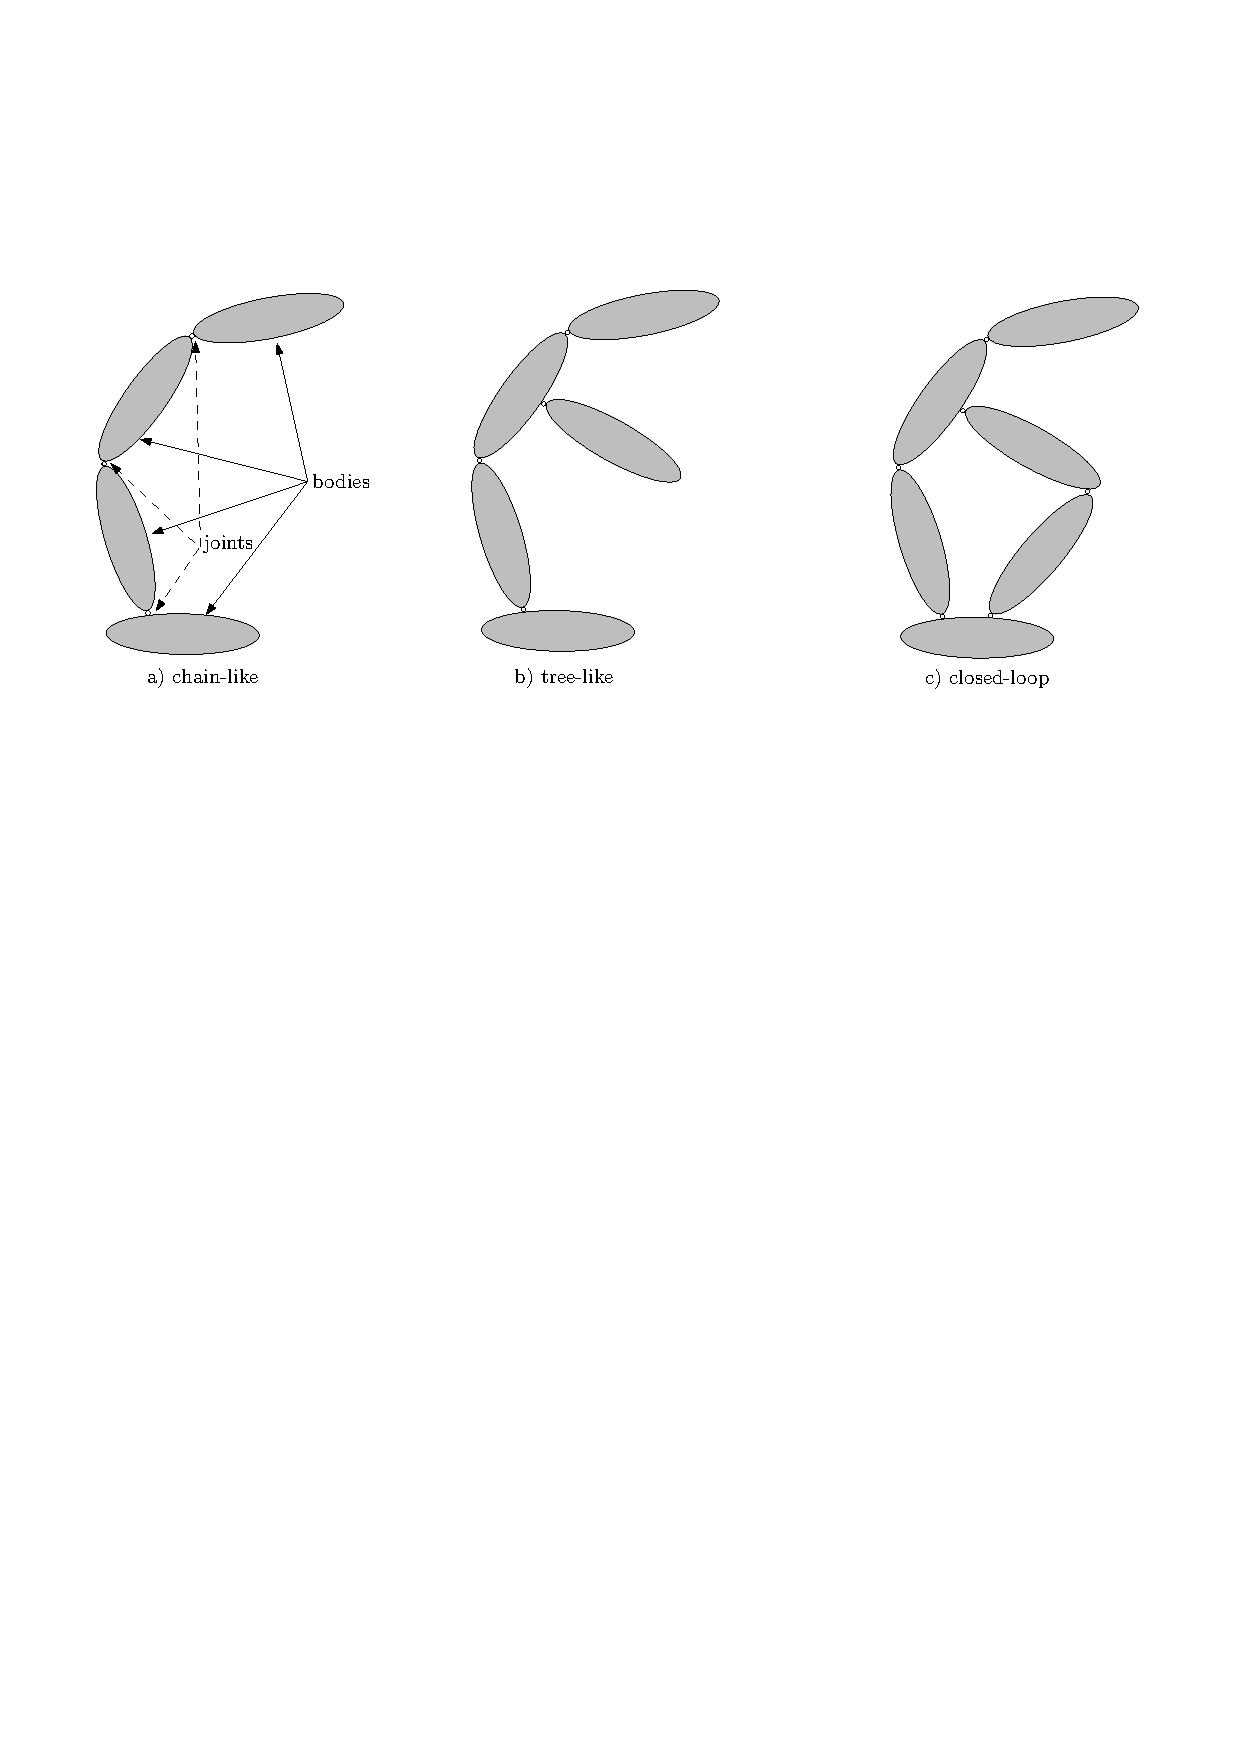
\includegraphics[width=1.\textwidth]{SerieTreeClosed}
\caption{Multibody systems.}
\label{fig:SerieTreeClosed} 
\end{figure}


\paragraph{Frame definition:}
 under this small displacement assumption, it is possible to define an inertial frame $\mathcal{R}_i=(P_i^0,\vec{x}_i,\vec{y}_i,\vec{z}_i)$ attached to the equilibrium configuration of each link $i$. In the chain-like and tree-like cases, $P_i^0$ is the connection point of the link $i$ with the parent link at the equilibrium. 
 $\mathbf{P}_{i/j}$ is the Direction Cosine Matrix (DCM)
between frames $\mathcal{R}_i$ and $\mathcal{R}_j$ (i.e.: the matrix of components of unitary vectors $\vec{x}_j$, $\vec{y}_j$, $\vec{z}_j$ in $\mathcal{R}_i$). $\mathbf{P}_{i/j}$ depends only on the given configuration $\vec{\theta}$ for all $i$ and $j$.

 \subsection{Two-port model of a link} The link $\mathcal{L}_{i}$ connected to the parent substructure $\mathcal{L}_{i-1}$ at the point $P_i$ % through a revolute joint along ($P_i,\vec{z}_i$) axis
 and to the child substructure $\mathcal{L}_{i+1}$ at point $C_i$ is depicted in Fig. \ref{fig:linki}. The double-port or TITOP (Two-Input Two-Output Port) model $\mathbf{G}_{P_i,C_i}^{\mathcal{L}_i}(s)$, proposed in \cite{Alazard2015}, is a linear dynamic model between $12$ inputs:
\begin{itemize}
\item the 6 components in $\mathcal{R}_i$ of the wrench $\vec{W}_{C_i}=[\vec{F}_{C_i}^T\;\vec{T}_{C_i}^T]^T$ applied by the substructure $\mathcal{L}_{i+1}$ to the link $\mathcal{L}_{i}$ at point $C_i$: $\vec{F}_{C_i}$ stands for the 3 components force vector applied at point $C_i$ and $\vec{T}_{C_i}$ stands for the 3 components torque vector applied at point $C_i$,
\item the 6 components in $\mathcal{R}_i$ of the acceleration twist $\vec{\ddot{x}}_{P_i}=[\vec{a}_{P_i}^T\;\dot{\vec{\omega}}_{P_i}^T]^T$  (time-derivative of the twist) of point $P_i$: $\vec{a}_{P_i}$ stands for the 3 components linear acceleration vector at point $P_i$ and $\dot{\vec{\omega}}_{P_i}$ stands for the 3 components angular acceleration vector at point $P_i$,
\end{itemize}
and $12$ outputs:
\begin{itemize}
\item the 6 components in $\mathcal{R}_i$ of the acceleration twist $\vec{\ddot{x}}_{C_i}=[\vec{a}_{C_i}^T\;\dot{\vec{\omega}}_{C_i}^T]^T$  of point $C_i$,
\item the 6 components in $\mathcal{R}_i$ of the wrench $\vec{W}_{P_i}=[\vec{F}_{P_i}^T\;\vec{T}_{P_i}^T]^T$ applied by the link $\mathcal{L}_{i}$ to the substructure $\mathcal{L}_{i-1}$ at point $P_i$,
\end{itemize}
and can be represented by the block-diagram depicted in Fig. \ref{fig:blki}. 

\begin{figure}[htbp!]
  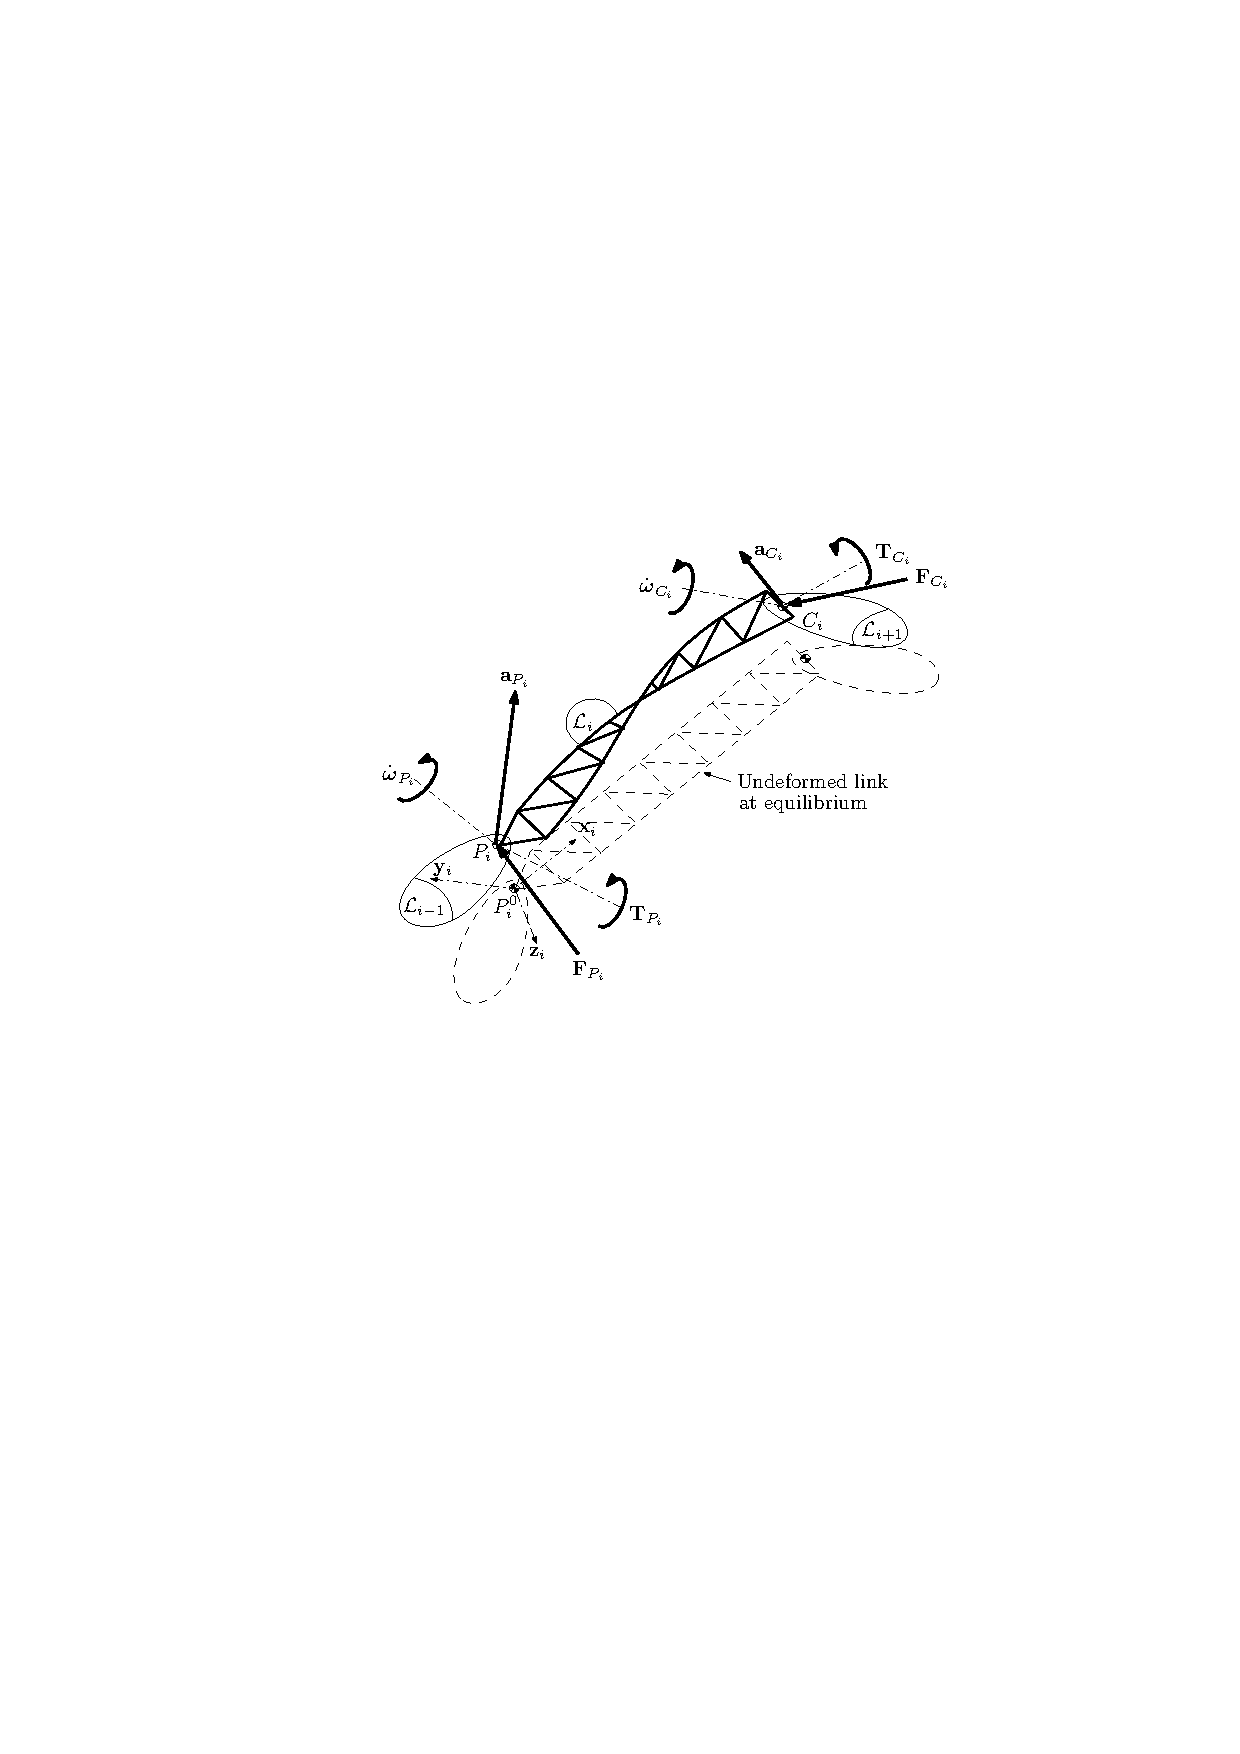
\includegraphics[width=0.7\textwidth]{linki}
\caption{The $i$-th flexible link in the structure.}
\label{fig:linki} 
\end{figure}

\begin{figure}[htbp!]
  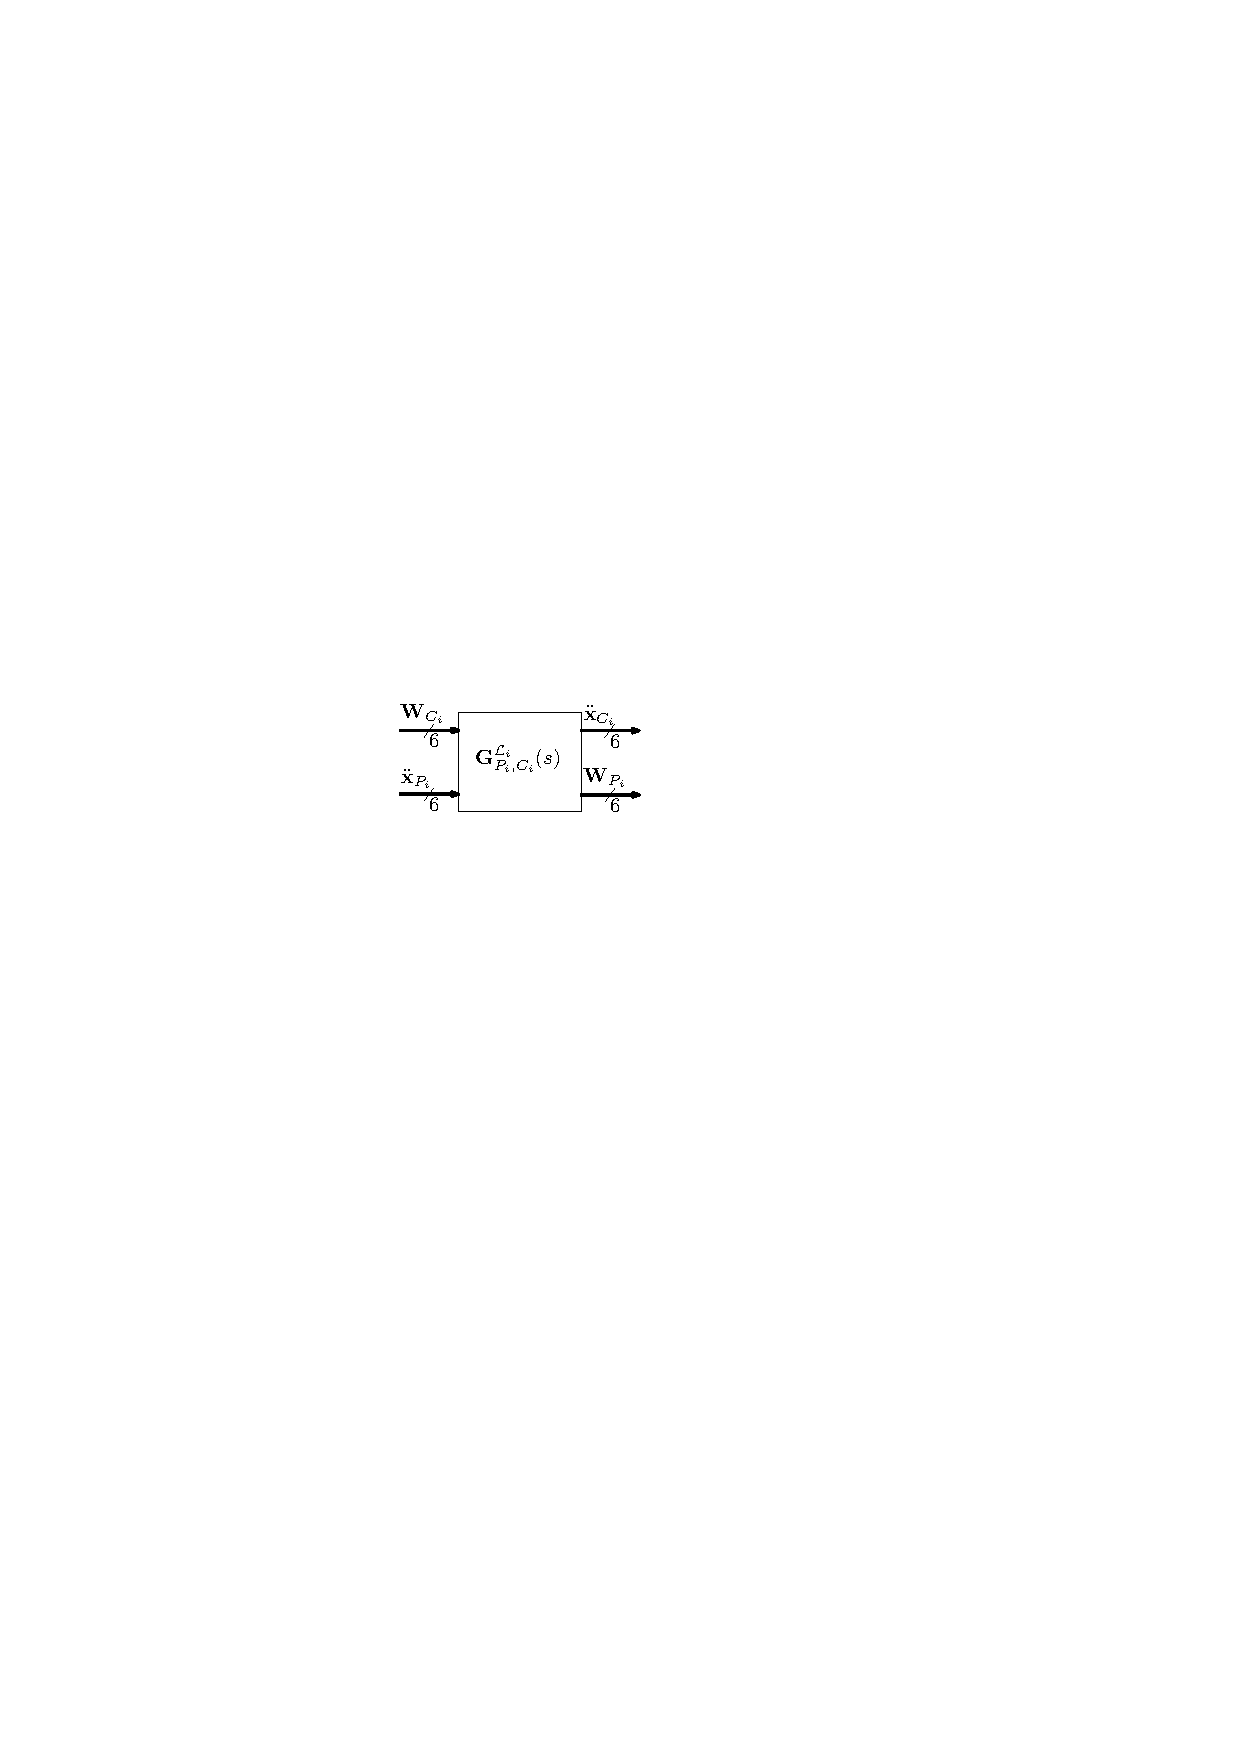
\includegraphics[width=0.3\textwidth]{blki}
\caption{Block-diagram of the TITOP model $\mathbf{G}_{P_i,C_i}^{\mathcal{L}_i}(s)$ of link $\mathcal{L}_i$.}
\label{fig:blki} 
\end{figure}

The way to obtain such a TITOP model $\mathbf{G}_{P_i,C_i}^{\mathcal{L}_i}(s)$ will be detailed in section \ref{sect:2} for an \textsc{Euler-Bernoulli} beams and is also detailed in \cite{Alazard2015} and \cite{Perez2015_LM} in the general case. The general procedure is based on the modal analysis of the link $\mathcal{L}_i$ with the \textit{clamped at $P_i$ - free at $C_i$} boundary conditions.  Indeed, the \textsc{Lagrange}'s formulation of dynamics using Assumed Mode Method (AMM) or Finite Element Method (FEM) leads to the generalized $2$-nd order differential equation \cite{TheodoreG95,ShabanaMSD1997}:

\begin{small}
	\begin{equation}\label{eq:2nd1}
	\left[\begin{array}{cc}\mathbf{D}^{\mathcal{L}_i}_{P_i} & \mathbf{L}_{P_i}^T\\ \mathbf{L}_{P_i} & \mathbf{1}_{n_i}\end{array}\right]\left[\begin{array}{c}\ddot{\mathbf{x}}_{P_i}\\ \ddot{\vec{\eta}}_i\end{array}\right]+\left[\begin{array}{cc} \mathbf{0}& \mathbf{0} \\  \mathbf{0} & \mbox{diag}(2\xi_j\omega_j)\end{array}\right]\left[\begin{array}{c}\star \\ \dot{\vec{\eta}}_i\end{array}\right]+\left[\begin{array}{cc} \mathbf{0}& \mathbf{0}\\  \mathbf{0}& \mbox{diag}(\omega_j^2)\end{array}\right]\left[\begin{array}{c}\star \\ \vec{\eta}_i\end{array}\right]=\left[\begin{array}{cc}-\mathbf{I}_6 & \vec{\tau}_{C_iP_i}^T\\ \mathbf{0} &  \mathbf{\Phi}_{C_i}^T \end{array}\right]\left[\begin{array}{c}\mathbf{W}_{P_i} \\ \mathbf{W}_{C_i}\end{array}\right]\;.
	\end{equation}
\end{small}
where:
\begin{itemize}
	\item $n_i$ is the number of flexible clamped-free modes of link $\mathcal{L}_i$ characterized by the  modal coordinates vector $\vec{\eta}_i$, the frequencies $\omega_j$, $j=1,\cdots,n_i$ and the damping ratio $\xi_j$, $j=1,\cdots,n_i$,
	\item $\mathbf{1}_{n_i}$ is the identity matrix of size $n_i$,
	\item $\mathbf{L}_{P_i}$ is the $n_i\times 6$ modal participation factor matrix of the link at point $P_i$ and projected in the frame $\mathcal{R}_i$, 
	\item $\mathbf{\Phi}_{C_i}$ is the  $6\times n_i$ projection matrix of the $n_i$ clamped-free modal shapes on the $6$ d.o.fs at point $C_i$ and projected in the frame $\mathcal{R}_i$,
	\item $\mathbf{\vec{\tau}}_{C_iP_i}$ is the ``rigid'' kinematic model between point $C_i$ and $P_i$ projected in the frame $\mathcal{R}_i$: $\mathbf{\vec{\tau}}_{C_iP_i}=\left[\begin{array}{cc}
	\mathbf{1}_3  & (^*\overrightarrow{C_iP_i})\\
	\mathbf{0}_{3\times 3} & \mathbf{1}_3  \\
	\end{array}\right]$ where $(^*\overrightarrow{C_iP_i})$ is the skew-symmetric matrix associated to vector from $C_i$ to $P_i$,
	\item $\mathbf{D}^{\mathcal{L}_i}_{P_i}$ is the $6 \times 6$  rigid mass model of the link at point $P_i$ and projected in the frame $\mathcal{R}_i$.
\end{itemize}


The right-hand term of eq. (\ref{eq:2nd1}) describes the contribution of the wrenches $\mathbf{W}_{P_i}$ and $\mathbf{W}_{C_i}$ to the generalized force vector. The acceleration twist $\vec{\ddot{x}}_{C_i}$ at point $C_i$ can be easily expressed from the generalized acceleration vector, the modal shapes and the kinematic model:

\begin{small}
	\begin{equation}\label{eq:2ndb}
\mbox{and:}\quad \ddot{\mathbf{x}}_{C_i}=[\vec{\tau}_{C_iP_i}\quad \mathbf{\Phi}_{C_i}]\left[\begin{array}{c}\ddot{\mathbf{x}}_{P_i}\\ \ddot{\vec{\eta}}_i\end{array}\right]
\end{equation}
\end{small}

From eq. (\ref{eq:2nd1}) and (\ref{eq:2ndb}), the general state-space realization (see also the definition of a state-space realization of a given transfer in appendix 1) of the TITOP model $\mathbf{G}_{P_i,C_i}^{\mathcal{L}_i}(s)$  reads:

\begin{scriptsize}
\begin{equation}\label{eq:MAPCstate}
\left[ \begin {array}{c} \dot{\vec{\eta}}_i \\ \ddot{\vec{\eta}}_i \\ \hline
\ddot{\mathbf{x}}_{C_i} \\ \mathbf{W}_{P_i}
\end{array} \right] = \left[ \begin {array}{cc|cc} \mathbf{0}_{n_i \times n_i}& \mathbf{1}_{n_i}
& \mathbf{0}_{n_i \times 6} & \mathbf{0}_{n_i \times 6}\\-\mbox{diag}(\omega_j^2) & -\mbox{diag}(2\xi_j\omega_j) & \mathbf{\Phi}_{C_i}^T & -\mathbf{L}_{P_i}\\ \hline
-\mathbf{\Phi}_{C_i}\,\mbox{diag}(\omega_j^2) & -\mathbf{\Phi}_{C_i}\,\mbox{diag}(2\xi_j\omega_j) &
\mathbf{\Phi}_{C_i}\mathbf{\Phi}_{C_i}^T & \left(\mathbf{\vec{\tau}}_{C_iP_i}-\mathbf{\Phi}_{C_i}\,\mathbf{L}_{P_i}\right)\\
\mathbf{L}^T_{P_i}\,\mbox{diag}(\omega_j^2) & \mathbf{L}^T_{P_i}\,\mbox{diag}(2\xi_i\omega_i) &
\left(\mathbf{\vec{\tau}}_{C_iP_i}-\mathbf{\Phi}_{C_i}\,\mathbf{L}_{P_i}\right)^T & -\mathbf{D}^{\mathcal{L}_i}_{P_i}+\mathbf{L}_{P_i}^T\mathbf{L}_{P_i}
\end{array}\right]  
\left[ \begin {array}{c} \vec{\eta}_i \\ \dot{\vec{\eta}}_i \\ \hline \mathbf{W}_{C_i} \\ \ddot{\mathbf{x}}_{P_i}
\end{array} \right]
\end{equation}
\end{scriptsize}


This model embeds, in the same minimal state-space realization, the direct dynamic model (transfer from acceleration to force) of the link $i$ at the point $P_i$ and the inverse dynamic model (transfer from force to acceleration) of the link $i$ at the point $C_i$.  All data required in eq. (\ref{eq:MAPCstate}) are commonly provided by FEM software. In \cite{Perez2015_LM}, the link between TITOP model and substructuring methods like the \textsc{Graig-Bampton} decomposition and the Component Modes Synthesis (CMS) is detailed in the general case. In \cite{Murali2015}, a custom \nastran / \simulink interface was developed to declare and manipulate the TITOP model $\mathbf{G}_{P_i,C_i}^{\mathcal{L}_i}(s)$ as a linear dynamic system object under the \matlab / \simulink environment.
 
 Let us note that the modal analysis of left-hand term of eq. (\ref{eq:2nd1}) corresponds to the \textit{free (at $P_i$) - free (at $C_i$)} case and provides $6$ rigid modes in addition to the free-free flexible modes. These rigid modes are not taken into account in the model $\mathbf{G}_{P_i,C_i}^{\mathcal{L}_i}(s)$ defined by eq. (\ref{eq:MAPCstate}). This is one the main advantage of the TITOP model: the boundary conditions and the rigid modes can be taken into account "outside" the model. That is detailed in the following section.
 % while the boundary conditions and the elimination of rigid modes are tricky in model reduction (\textsc{Craig-Bampton} ans CMS methods) used in FEM substructures.  
 
\subsection{Interconnection and channel inversion of TITOP models} 
The open-loop dynamics of the TITOP model $\mathbf{G}_{P_i,C_i}^{\mathcal{L}_i}(s)$, i.e. when the inputs are null, corresponds to the link dynamics when it is clamped at $P_i$ ($\ddot{\mathbf{x}}_{P_i}=\mathbf{0}$) and free at $C_i$ ($\mathbf{W}_{C_i}=\mathbf{0}$). It must be noticed that all the $12$ input-output channels of the model  $\mathbf{G}_{P_i,C_i}^{\mathcal{L}_i}(s)$  are invertible assuming that a residual mass (inertia) of the link $i$ is attached to the points $P_i$ and $C_i$ along (around) the $3$ axes. Such an assumption is valid by using finite-element method or assumed-mode method to  model the flexibility of the link. 

$\left[\mathbf{G}_{P_i,C_i}^{\mathcal{L}_i}\right]^{-1_\mathbf{I}}(s)$ denotes the model where the channels numbered in the index vector $\mathbf{I}$ are inverted according to the procedure described in appendix 1. This channel inversion operation is very useful to analyze the dynamics of the link $\mathcal{L}_i$ for various boundary conditions:
\begin{itemize}
\item clamped at $P_i$ and clamped at $C_i$, using $\left[\mathbf{G}_{P_i,C_i}^{\mathcal{L}_i}\right]^{-1_{[1:6]}}(s)$ whose inputs are $\ddot{\mathbf{x}}_{C_i}$ and $\ddot{\mathbf{x}}_{P_i}$,
\item free at $P_i$ and free at $C_i$, using $\left[\mathbf{G}_{P_i,C_i}^{\mathcal{L}_i}\right]^{-1_{[7:12]}}(s)$ whose inputs are $\mathbf{W}_{C_i}$ and $\mathbf{W}_{P_i}$,
\item free at $P_i$ and clamped at $C_i$, using $\left[\mathbf{G}_{P_i,C_i}^{\mathcal{L}_i}\right]^{-1}(s)$ whose inputs are $\ddot{\mathbf{x}}_{C_i}$ and $\mathbf{W}_{P_i}$,
\item or to take into account a revolute (resp. prismatic) joint at the point $P_i$ around (resp. along) $\vec{z}_i$-axis using $\left[\mathbf{G}_{P_i,C_i}^{\mathcal{L}_i}\right]^{-1_{12}}(s)$ (resp. $\left[\mathbf{G}_{P_i,C_i}^{\mathcal{L}_i}\right]^{-1_{9}}(s)$), i.e.: no torque (resp. force) can be applied by the link $\mathcal{L}_i$ to the parent substructure $\mathcal{L}_{i-1}$ around (resp. along) $\vec{z}_i$-axis. A spherical joint can be taken into account using $\left[\mathbf{G}_{P_i,C_i}^{\mathcal{L}_i}\right]^{-1_{[10:12]}}(s)$.
\end{itemize}

More generally, once the TITOP model of each links is defined and the DCM $\mathbf{P}_{i/j}$ for a given nominal configuration $\vec{\theta}$ are computed,  the linear model of the whole multibody system can be built by simply connecting the input/outputs of the TITOP models. Hereafter some examples of interconnection are presented.

\paragraph{Chain-like multibody system:}
let us consider a flexible spacecraft $\mathcal{S}$, whose reference body frame is $(O,\vec{x_0},\vec{y}_0,\vec{z}_0)$, fitted with a flexible boom $\mathcal{B}$ at point $P_1$ with a revolute joint along $(P_1,\vec{z}_1)$-axis.  The boom holds a flexible antenna $\mathcal{A}$ at point $P_2$. A sketch of such a multibody system is depicted in Fig. \ref{fig:3bodies} (left). The block-diagram associated to this system is presented in Fig.  \ref{fig:3bodies} (right). It involves the 3 TITOP models of the 3 bodies with the channel inversions required by the different boundary conditions. $\mathbf{P}^a_{i/j}$ is the augmented $6 \times 6$ DCM:
\[
\mathbf{P}^a_{i/j}=\left[\begin{array}{cc}\mathbf{P}_{i/j}& \mathbf{0}_{3\times 3}\\\mathbf{0}_{3\times 3} & \mathbf{P}_{i/j}\end{array}\right]\;.
\]
\begin{figure}[htbp!]
  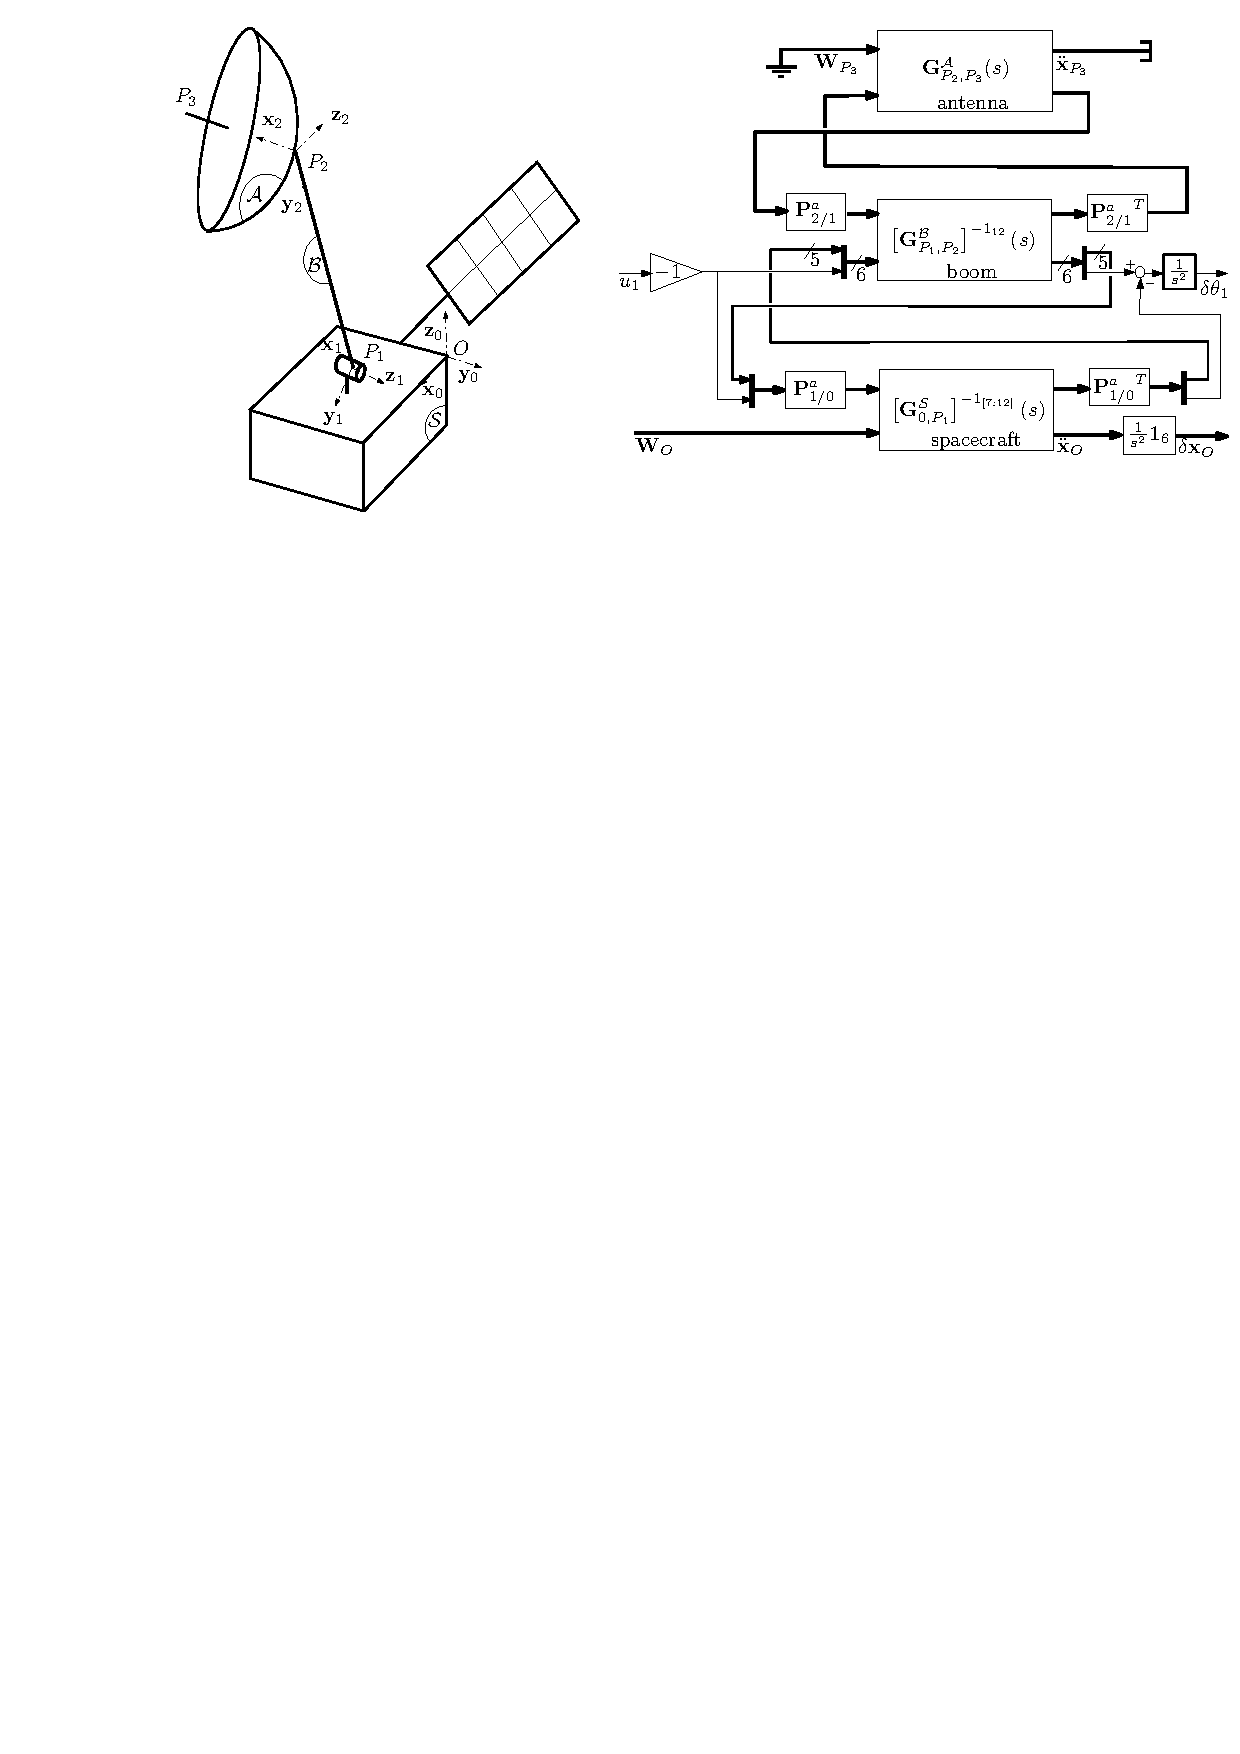
\includegraphics[width=\textwidth]{3bodies_bis.pdf}
\caption{A flexible boom $\mathcal{B}$ linking a flexible antenna $\mathcal{A}$ to a flexible spacecraft $\mathcal{S}$ through a revolute joint (left) and its block diagram model (right).}
\label{fig:3bodies} 
\end{figure}

In this block-diagram, $7$ double integrators are added on the outputs to represent the $7$ rigid modes associated to the $7$ d.o.fs of this system: the 6 d.o.f. of the spacecraft and the 1 d.o.f of the revolute joint. The $7$ inputs of this model are the torque $u_1$ applied inside the revolute joint by the driven mechanism and the $6$ components of the wrench $\mathbf{W}_0$ applied by the attitude and orbit control system at the reference point $O$. All dynamic couplings between the flexible modes of the antenna, the boom and the spacecraft are directly taken into account through the feedback connections between the 3 TITOP models. Furthermore, the inertia $j_1$, the stiffness $k_1$ and the damping factor $f_1$ of the driven mechanism located in the revolute joint can be added by a feedback loop: $u_1=-j_1\,\ddot{\delta \theta}_1-f_1\,\dot{\delta \theta}_1-k_1\,\delta \theta_1$, directly plugged into the block-diagram. That can be used to handle any arbitrary boundary condition in the revolute joint, from the free condition ($j_1=k_1=f_1=0$) to the clamped condition ($k_1\to \infty$).

\paragraph{Tree-like multibody system:}
in that case, one link $\mathcal{B}$ can have two (or more) child bodies connected to  $\mathcal{B}$ at points $C_1$ and $C_2$. This case is quite similar to the previous one and requires a model of the link  augmented with additional ports. This case is not detailed in this paper. The reader is advised to refer to \cite{Alazard2015} where the 3 ports model of a link (denoted $\mathbf{G}_{P,C_1,C_2}^{\mathcal{B}}(s)$) and an example of tree-like system are detailed (see Fig. 18 in \cite{Alazard2015}).

\paragraph{Closed-loop multibody system:} such mechanisms are commonly modeled through \textsc{Lagrange} approach using \textsc{Lagrange} multipliers \cite{ShabanaMSD1997,Simeon2006}. They are used to be denoted $\vec{\lambda}$ and correspond to the generalized constraint forces. Considering the model of the link $\mathcal{L}_i$ given in equations (\ref{eq:2nd1}) and (\ref{eq:2ndb}), with a kinematic-chain closed at point $C_i$, the \textsc{Lagrange} multipliers are nothing else that the wrench at this point applied by the link $\mathcal{L}_i$: $\vec{\lambda}=-\mathbf{W}_{C_i}$. The classical \textsc{Lagrange} approach leads to an augmented system of differential-algebraic equations which reads here:

\begin{small}
\begin{equation}\label{eq:2nda}
\left[\begin{array}{ccc}\mathbf{D}^{\mathcal{L}_i}_{P_i} & \mathbf{L}_{P_i}^T & \vec{\tau}_{C_iP_i}^T \\ \mathbf{L}_{P_i} & \mathbf{1}_{n_i} & \mathbf{\Phi}_{C_i}^T \\
\vec{\tau}_{C_iP_i} & \mathbf{\Phi}_{C_i} & \mathbf{0}\end{array}\right]\left[\begin{array}{c}\ddot{\mathbf{x}}_{P_i}\\ \ddot{\vec{\eta}}_i\\\vec{\lambda}\end{array}\right]+\left[\begin{array}{ccc} \mathbf{0}& \mathbf{0}& \mathbf{0} \\  \mathbf{0} & \mbox{diag}(2\xi_j\omega_j)& \mathbf{0} \\\mathbf{0}& \mathbf{0}& \mathbf{0}\end{array}\right]\left[\begin{array}{c}\star \\ \dot{\vec{\eta}}_i \\ \star \\\end{array}\right]+\left[\begin{array}{ccc} \mathbf{0}& \mathbf{0}& \mathbf{0}\\  \mathbf{0}& \mbox{diag}(\omega_j^2)& \mathbf{0} \\\mathbf{0}& \mathbf{0}& \mathbf{0}\end{array}\right]\left[\begin{array}{c} \star \\ \vec{\eta}_i \\ \star\\ \end{array}\right]=\left[\begin{array}{c}-\mathbf{W}_{P_i} \\ \mathbf{0} \\ \ddot{\mathbf{x}}_{C_i}\end{array}\right]\;.
\end{equation}
\end{small}
Considering the TITOP formulation of the model in equation (\ref{eq:MAPCstate}), $\vec{\lambda}$ (up to the sign) is an input of $\mathbf{G}_{P_i,C_i}^{\mathcal{L}_i}(s)$ or an output of the model $\left[\mathbf{G}_{P_i,C_i}^{\mathcal{L}_i}\right]^{-1_{[1:6]}}(s)$ where the upper port is inverted. Thus, the upper port of $\left[\mathbf{G}_{P_i,C_i}^{\mathcal{L}_i}\right]^{-1_{[1:6]}}(s)$ can be connected in a feedback loop to the upper port of the adjoining link in order to close the kinematic chain. Such an interconnection is presented in Fig. \ref{fig:2bodies} (right) in the case of a very simple closed-loop structure composed of two links $\mathcal{L}_1$ and $\mathcal{L}_2$ clamped to the ground, and one to each other at point $C_1 \equiv C_2$. In that case, the model outputs are the two wrenches $\mathbf{W}_{P_1}$ and $\mathbf{W}_{P_2}$ applied by the system to the ground at points $P_1$ and $P_2$. Similar to the case of the chain-like multibody system example, a revolute joint around the $(C_2,\vec{z}_1)$-axis can be taken into account using the model $\left[\mathbf{G}_{P_2,C_2}^{\mathcal{L}_2}\right]^{-1_{[1:5]}}(s)$ to cancel the torque around this axis in the joint between $\mathcal{L}_1$ and $\mathcal{L}_2$, i.e. $\vec{\lambda}(6)=\mathbf{W}_{C_i}(6)=0$ (see also the illustration on the four bar mechanism in section \ref{sect:fb}). 
\begin{figure}[htbp!]
  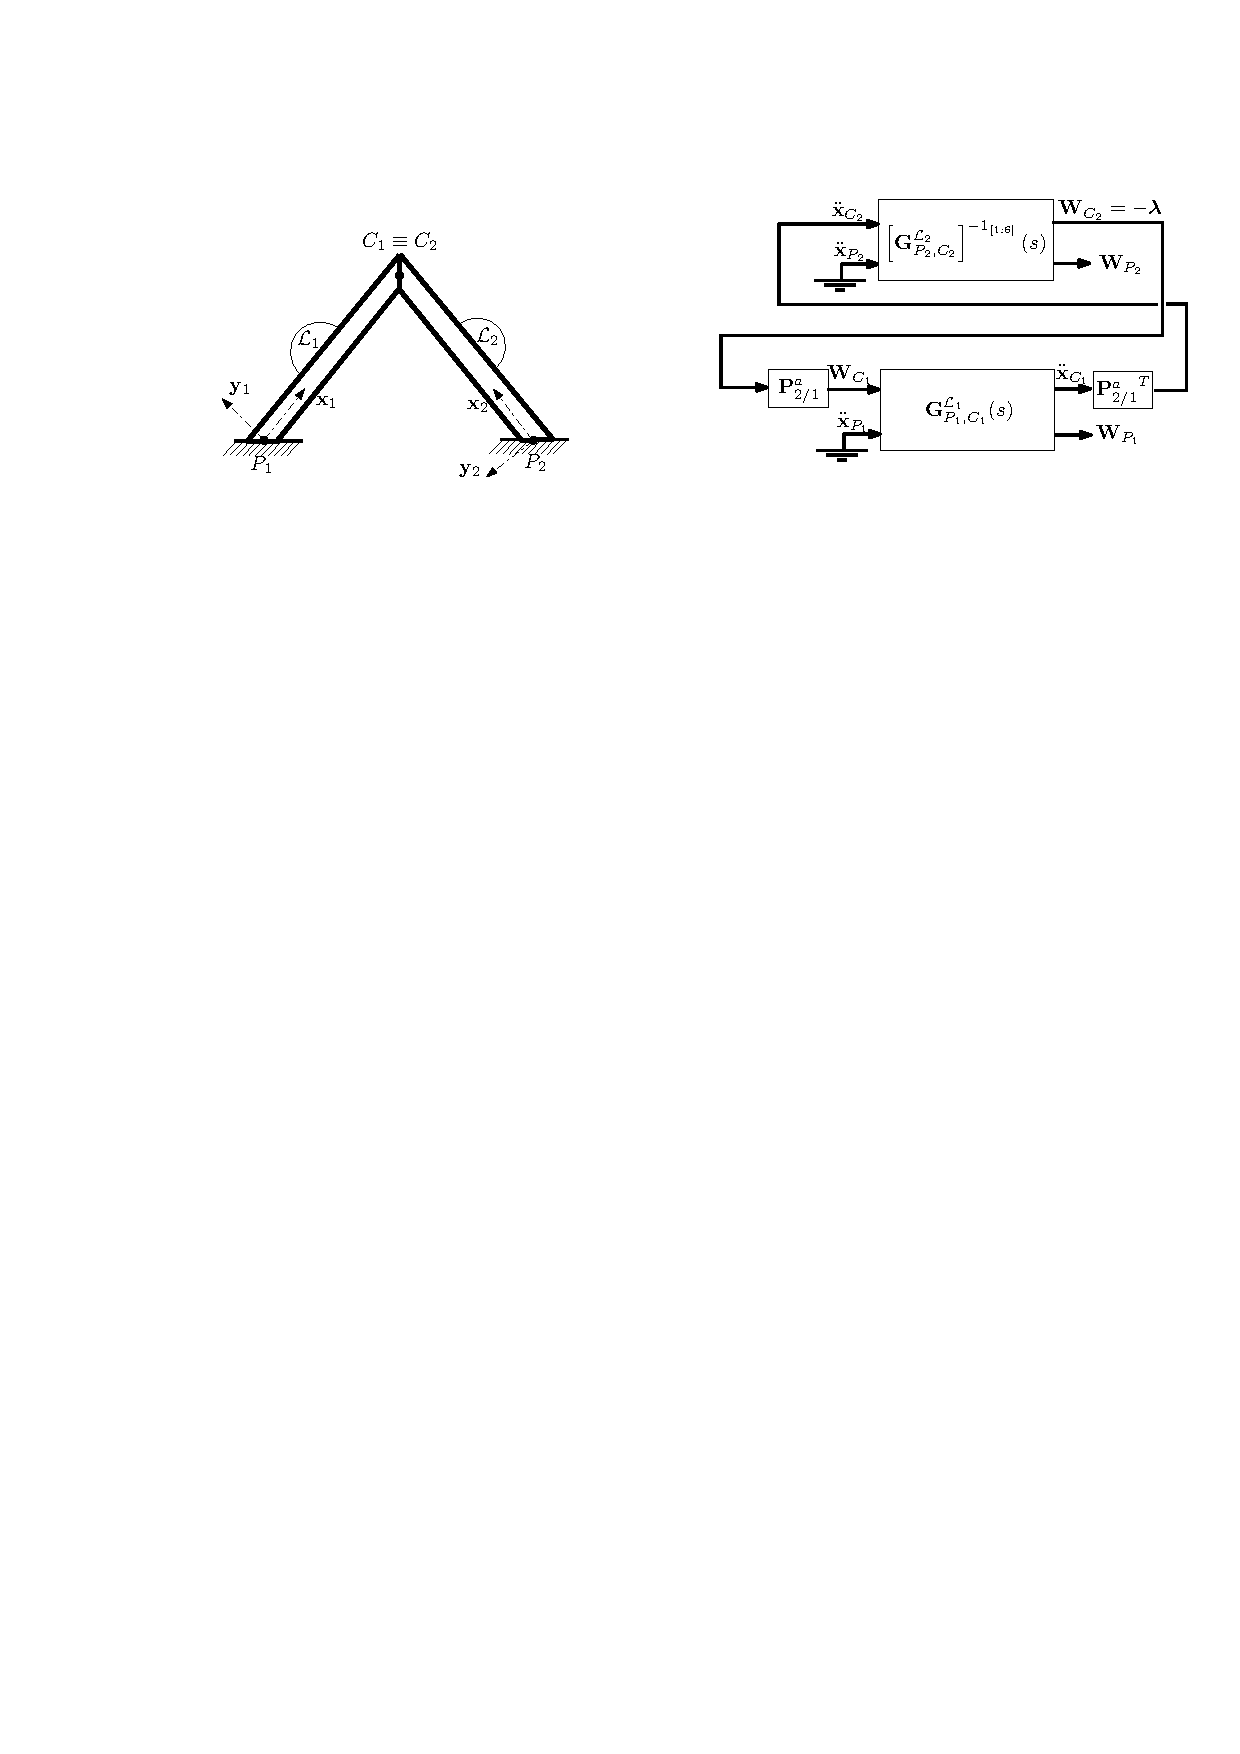
\includegraphics[width=\textwidth]{2bodies}
\caption{A flexible closed-loop structure (left) and its block diagram model (right).}
\label{fig:2bodies} 
\end{figure}

\section{Two-port model of a beam in the planar case}\label{sect:2}
Let us consider a uniform beam $\mathcal{B}$ between points $P$ and $C$, characterized by the following parameters (see Fig. \ref{fig:flexion_4}):
\begin{itemize}
\item mass density: $\rho\,(kg/m^3)$,
\item section: $S\,(m^2)$,
\item length: $l\,(m)$,
\item \textsc{Young} modulus: $E\, (N/m^2)$,
\item second moment of area w.r.t $\vec{z}$-axis: $I_z\, (m^4)$.
\end{itemize}
\begin{figure}[htbp!]
  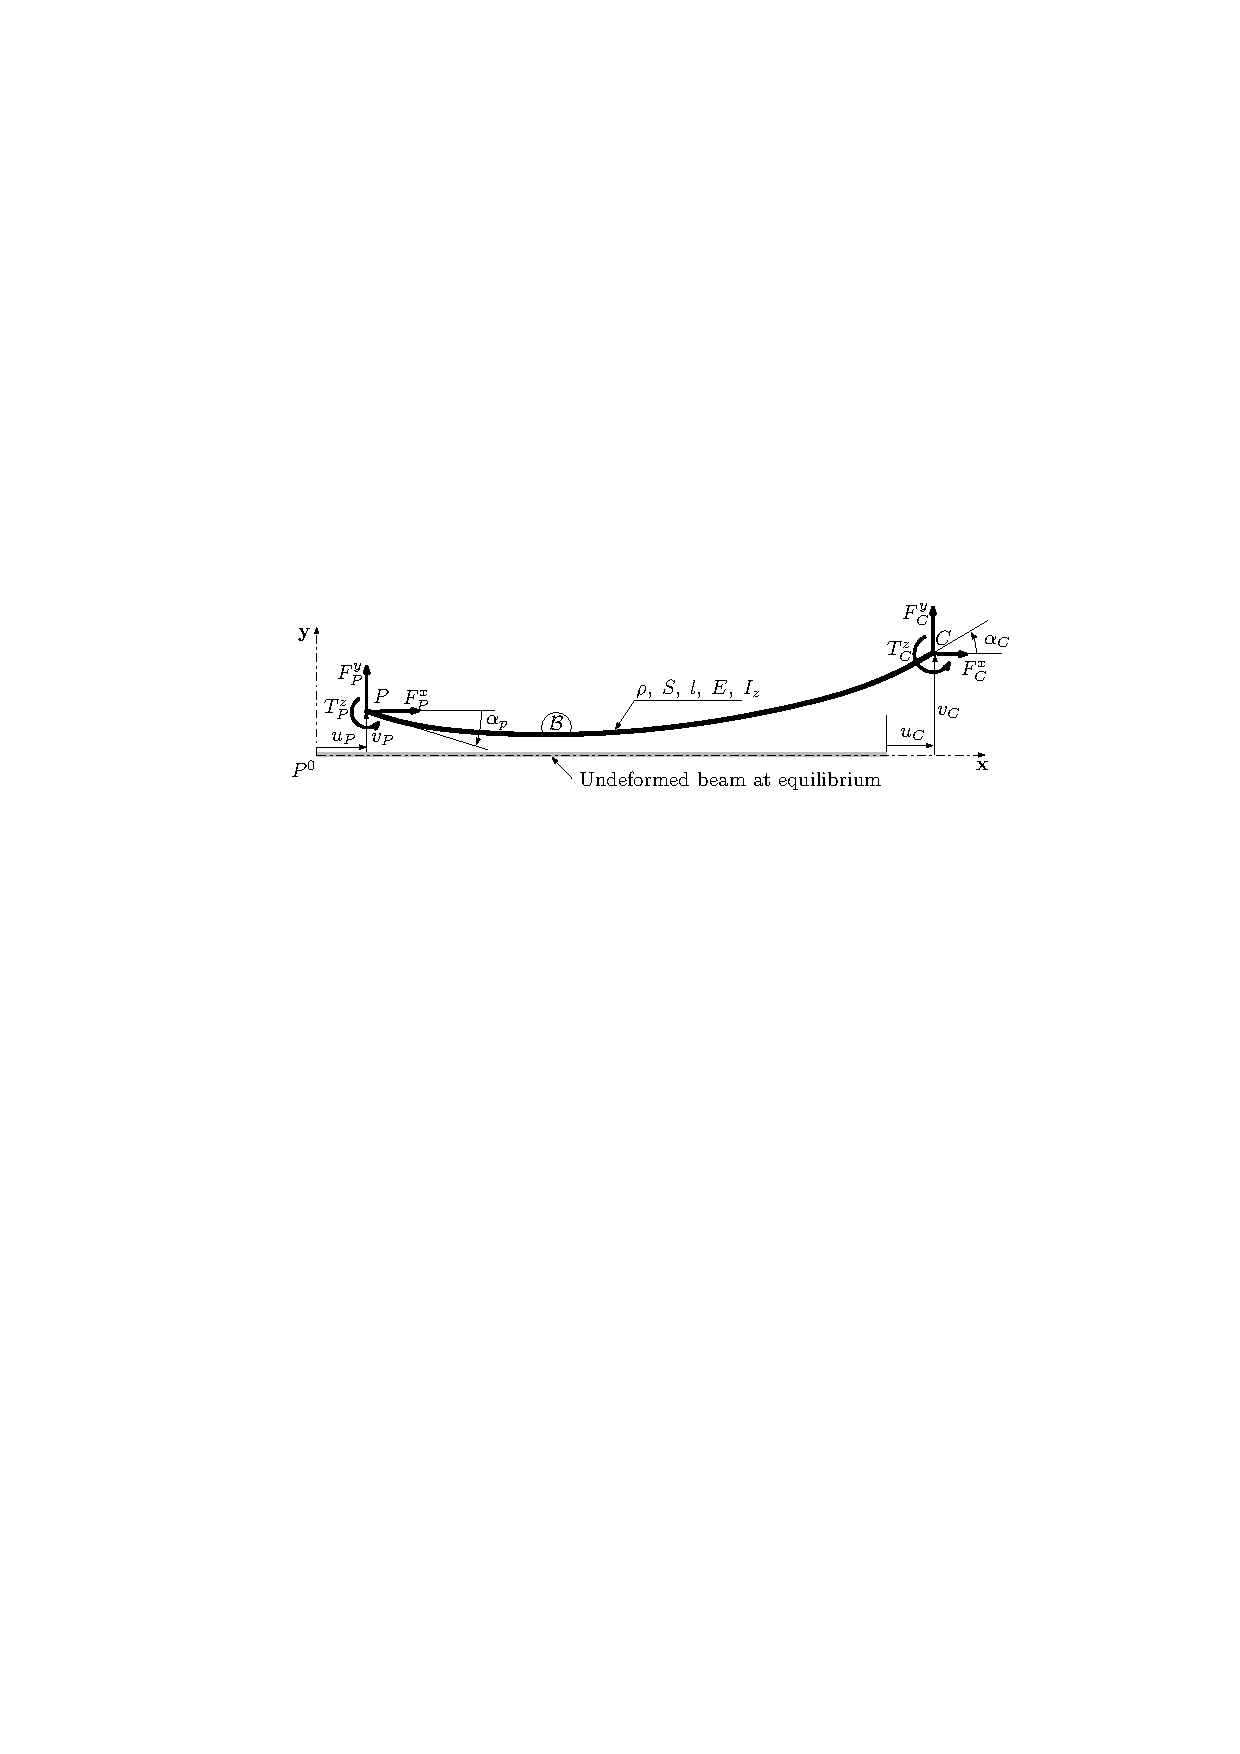
\includegraphics[width=0.8\textwidth]{flexion_4b}
\caption{A uniform beam $\mathcal{B}$ in the plane $(P^0,\vec{x},\vec{y})$.}
\label{fig:flexion_4} 
\end{figure}
The objective is to compute the TITOP model $\mathbf{G}_{P,C}^{\mathcal{B}}(s)$. In the ($3$ d.o.fs) planar case this model will be denoted $\mathbf{G}(s)$ and is a transfer between 6 inputs:
\begin{itemize}
\item the 3 components $F^x_{C}\,(N)$, $F^y_{C}\,(N)$ and $T^z_{C}\,(Nm)$ in the frame $\mathcal{R}=(P^0,\vec{x},\vec{y},\vec{z})$ of the planar wrench applied \textbf{to} the beam at point $C$,
\item the 3 components $\ddot{u}_{P}\,(m/s^2)$, $\ddot{v}_{P}\,(m/s^2)$ and $\ddot{\alpha}_{P}\,(rad/s^2)$ in the frame $\mathcal{R}$ of the planar acceleration twist of the beam at point $P$,
\end{itemize}
and 6 outputs:
\begin{itemize}
\item the 3 components $\ddot{u}_{C}\,(m/s^2)$, $\ddot{v}_{C}\,(m/s^2)$ and $\ddot{\alpha}_{C}\,(rad/s^2)$ in the frame $\mathcal{R}$ of the planar acceleration twist of the beam at point $C$,
\item the 3 components $F^x_{P}\,(N)$, $F^y_{P}\,(N)$ and $T^z_{P}\,(Nm)$ in the frame $\mathcal{R}$ of the planar wrench applied \textbf{by} the beam at point $P$.
\end{itemize}
This model $\mathbf{G}(s)$ is derived in following sections considering a decoupling between the pure flexion in the plane $(P^0,\vec{x},\vec{y})$ and the pure traction-compression along $(P^0,\vec{x})$-axis.

\subsection{Pure flexion in the plane $(P^0,\vec{x},\vec{y})$}
A well-known approach to derive the dynamic model of a flexible beam is based on the \textsc{Lagrange} technique combined with the Assumed Modes Method (AMM) \cite{DeLucaSiciliano}. This approach involves a moving body frame $\widetilde{\mathcal{R}}=(P,\widetilde{\mathrm{x}},\widetilde{\mathrm{y}},\mathrm{z})$ attached to the beam at point $P$ (see Fig. \ref{fig:flexion_5}). Under the small deflection assumption, the displacement $v(x,t)$ along $\vec{y}$-axis at any point of abscissa $x$ and at any time $t$ reads as follows:
\begin{equation}\label{eq:defv}
v(x,t)=v_P(t)+x\alpha_P(t)+\widetilde{v}(x,t)\quad \forall x\in [0,l]\;.
\end{equation}

\begin{figure}[htbp!]
  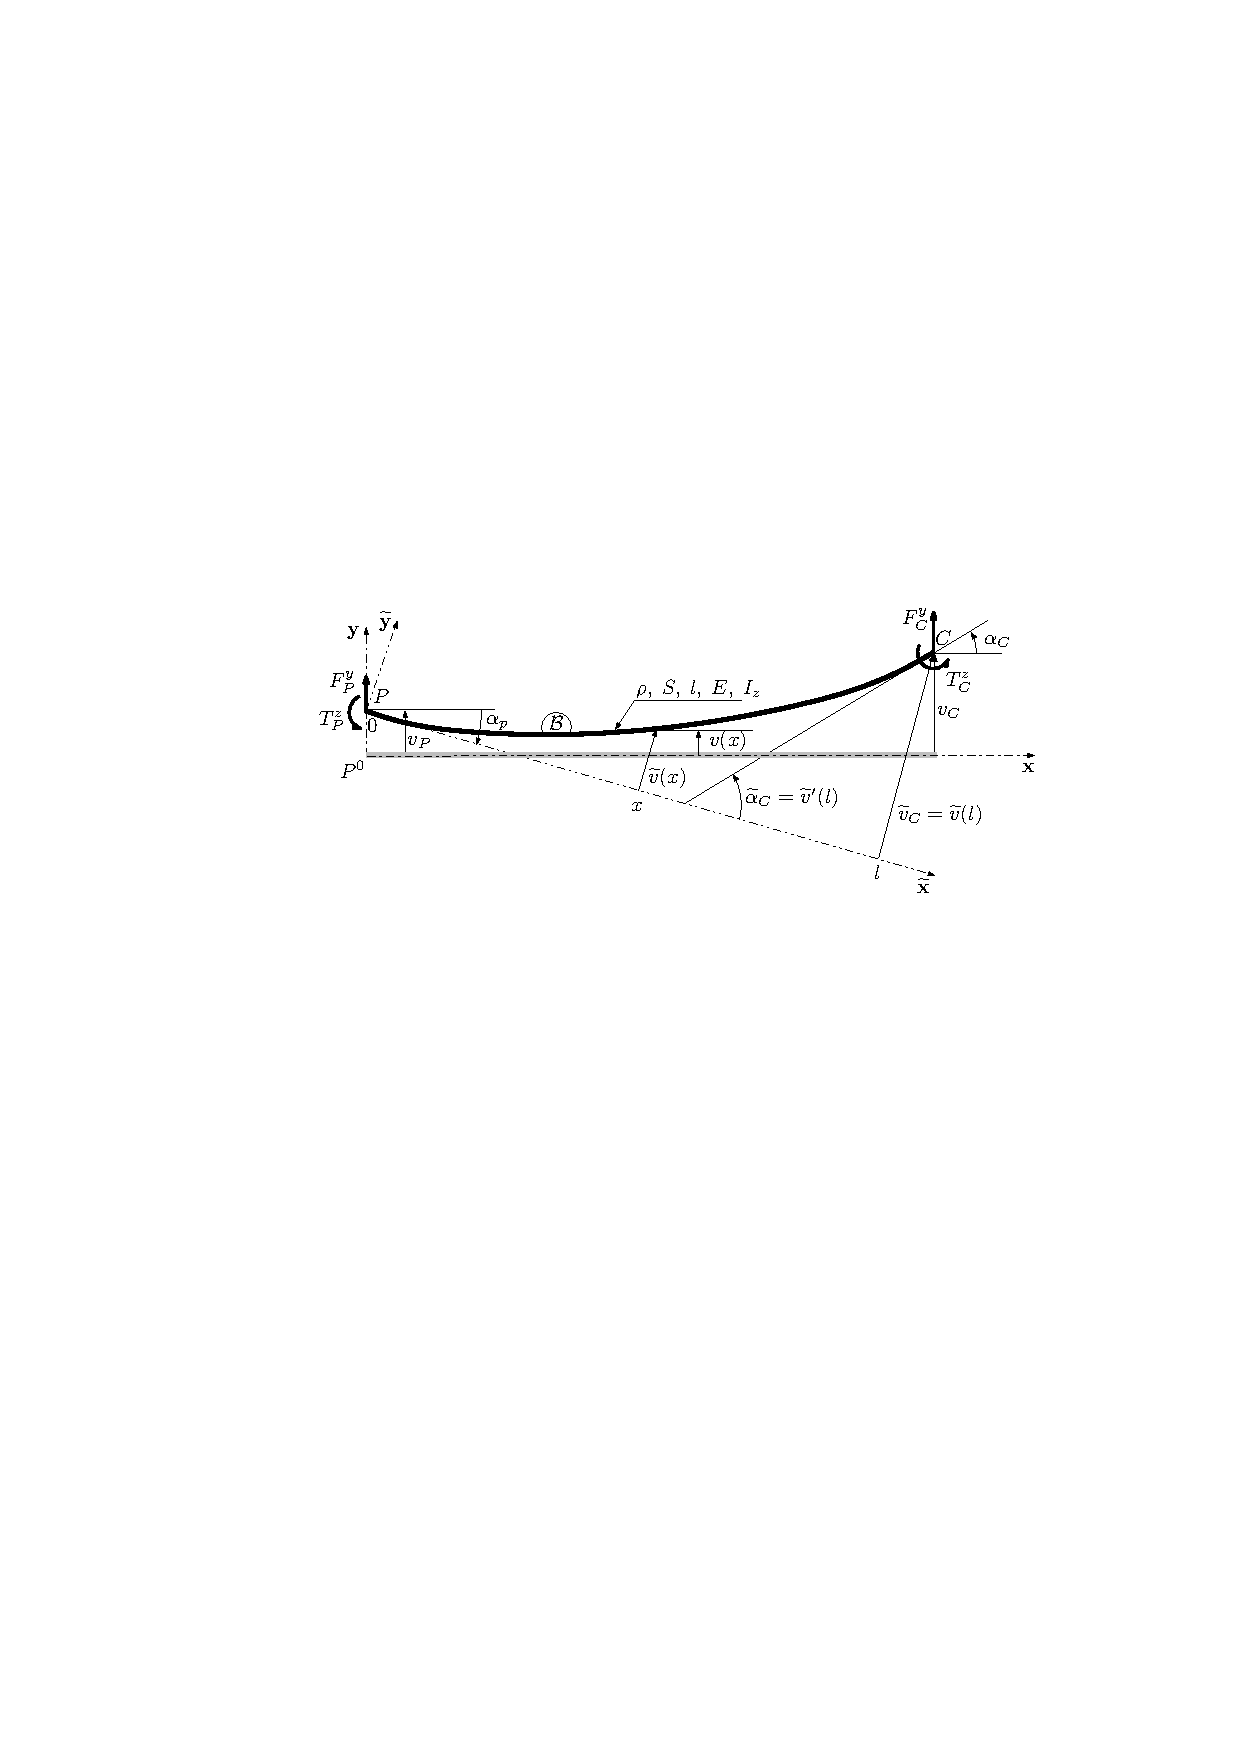
\includegraphics[width=0.8\textwidth]{flexion_5b}
\caption{Parameterization of the beam deflection at a given time $t$.}
\label{fig:flexion_5} 
\end{figure}
% In the assumed mode method,
The deflection $\widetilde{v}(x,t)$ in the moving frame $\widetilde{\mathcal{R}}$  is split up into $n$ shape functions $\phi_i(x)$ ($\vec{\phi}(x)=[\phi_1(x)\;\cdots\; \phi_n(x)]^T$ being the shape function vector), associated to $n$ time-domain functions $q_i(t)$, $n=1,\cdots,n$ ($\vec{q}(t)=[q_1(t)\;\cdots\; q_n(t)]^T$):
\begin{equation}\label{eq:decomp}
\widetilde{v}(x,t)=\sum_{i=0}^{n}\phi_i(x)q_i(t)=\vec{\phi}(x)^T\vec{q}(t)\;.
\end{equation}
Then, the kinetic energy reads:
\[
\mathcal{T}=\frac{1}{2}\rho\,S\int_0^l(\dot{v}_P+x\dot{\alpha}_P+\Sigma_{i=0}^{n}\phi_i(x)\dot{q}_i)^2dx=\frac{1}{2}\left[\begin{array}{c}\left[\begin{array}{c}\dot{v}_P\\\dot{\alpha}_P\end{array}\right] \\ \dot{\vec{q}} \end{array}\right]^T\left[\begin{array}{cc}\mathbf{M}_{rr} & \mathbf{M}_{rf}^T \\\mathbf{M}_{rf} & \mathbf{M}_{ff} \end{array}\right]\left[\begin{array}{c}\left[\begin{array}{c}\dot{v}_P\\\dot{\alpha}_P\end{array}\right] \\ \dot{\vec{q}} \end{array}\right]
\]
where:
\begin{itemize}
\item $\mathbf{M}_{rr}=\left[\begin{array}{cc}\scriptstyle{\rho\,S\,l} & \frac{\rho\,S\,l^2}{2} \\ \frac{\rho\,S\,l^2}{2} &\frac{\rho\,S\,l^3}{3} \end{array}\right]$ is the $2\times 2$ rigid mass matrix,
\item $\mathbf{M}_{rf}=[\rho\,S\int_0^l\vec{\phi}(x)dx\quad \rho\,S\int_0^lx\vec{\phi}(x)dx]$ is the $n\times 2$ rigid-flexible coupling mass matrix,
\item $\mathbf{M}_{ff}=\rho\,S\int_0^l\vec{\phi}(x)\vec{\phi}(x)^Tdx$ is the $n\times n$ flexible mass matrix.
\end{itemize}
The elastic potential energy reads:
\[ \mathcal{V}= \frac{1}{2}\,E\,I_z\int_0^l\left(\frac{\partial^2 \widetilde{v}(x,t)}{\partial x^2}\right)^2dx=\frac{1}{2}\left[\begin{array}{c}\left[\begin{array}{c}v_P\\ \alpha_P\end{array}\right] \\ \vec{q} \end{array}\right]^T\left[\begin{array}{cc}\mathbf{0}_{2\times 2} &  \mathbf{0}_{2\times n}\\ \mathbf{0}_{n\times 2} & \mathbf{K}_{n\times n} \end{array}\right]\left[\begin{array}{c} \left[\begin{array}{c} v_P\\ \alpha_P\end{array}\right]\\ \vec{q} \end{array}\right]\]
where $\mathbf{K}=E\,I_z\int_0^l\left[\frac{d^2\vec{\phi}(x)}{dx^2}\right]\left[\frac{d^2\vec{\phi}(x)}{dx^2}\right]^Tdx=E\,I_z\int_0^l\vec{\phi}''(x)\vec{\phi}''^T(x)dx$ is the $n\times n$ stiffness matrix.

Applying the action-reaction principle at point $P$, the work of external loads is:
\begin{eqnarray}
W_{ext} & = & -v_P\,F^y_P-\alpha_P\,T^z_P+v(l)\,F^y_C+v'(l)\,T^z_C \\
& = & [-v_P\quad -\alpha_P \quad v_P+l\alpha_P+\vec{q}^T\vec{\phi}(l) \quad \alpha_P+\vec{q}^T\vec{\phi}'(l)]\left[\begin{array}{c}F^y_P \\ T^z_P \\ F^y_C\\ T^z_C\end{array}\right] \\
& = & \left[\begin{array}{c}v_P\\ \alpha_P \\ \vec{q} \end{array}\right]^T\left[\begin{array}{cccc} -1 & 0 & 1 & 0\\0 & -1 & l & 1 \\ \mathbf{0}_{n\times 1} &\mathbf{0}_{n\times 1} & \vec{\phi}(l) & \vec{\phi}'(l) \end{array}\right]\left[\begin{array}{c}F^y_P \\ T^z_P \\ F^y_C\\ T^z_C\end{array}\right]
\end{eqnarray}
and the \textsc{Lagrange} derivation leads to the following second-order equation:
\begin{equation}\label{eq:2nd}
\left[\begin{array}{cc}\mathbf{M}_{rr} & \mathbf{M}_{rf}^T \\\mathbf{M}_{rf} & \mathbf{M}_{ff} \end{array}\right]\left[\begin{array}{c}\left[\begin{array}{c}\ddot{v}_P\\\ddot{\alpha}_P\end{array}\right] \\ \ddot{\vec{q}} \end{array}\right]+\left[\begin{array}{cc}\mathbf{0}_{2\times 2} &  \mathbf{0}_{2\times n}\\ \mathbf{0}_{n\times 2} & \mathbf{K}_{n\times n} \end{array}\right]\left[\begin{array}{c} \left[\begin{array}{c} v_P\\ \alpha_P\end{array}\right] \\ \vec{q} \end{array}\right]=\left[\begin{array}{cc} -\mathbf{I}_2 & \vec{\tau}^T \\\mathbf{0}_{n\times 2} &  \vec{\Phi}^T(l) \end{array}\right]\left[\begin{array}{c}\left[\begin{array}{c} F^y_P \\ T^z_P \end{array}\right] \\ \left[\begin{array}{c} F^y_C\\ T^z_C\end{array}\right] \end{array}\right]
\end{equation}
with $\vec{\tau}=\left[\begin{array}{cc}1 & l\\ 0 & 1 \end{array}\right]$, the rigid  kinematic model between point $C$ and $P$ of the beam in the planar case, and $\vec{\Phi}(l)=[\vec{\phi}(l)\quad \vec{\phi}'(l)]^T$. The relation between accelerations at point $C$ and at point $P$, under low speed motion assumption reads:
\begin{equation}\label{eq:acc1}
\left[\begin{array}{c}\ddot{v}_C\\\ddot{\alpha}_C \end{array}\right]=\vec{\tau}\left[\begin{array}{c}\ddot{v}_P\\\ddot{\alpha}_P \end{array}\right]+\vec{\Phi}(l)\ddot{\vec{q}}\;.
\end{equation}
From equations (\ref{eq:2nd}) and (\ref{eq:acc1}), one can easily derive the state-space representation, associated to the state vector $\vec{x}_f=[\vec{q}^T\quad \dot{\vec{q}}^T]^T$, of the TITOP model $\mathbf{G}_{f}(s)$ relative to the pure flexion dynamics in the plane $(P^0,\vec{x},\vec{y})$ (see Figure \ref{fig:TyRz}):
\begin{small}
\begin{equation}\label{eq:Gfss}
  \left[\begin{array}{c}\dot{\vec{q}} \\ \ddot{\vec{q}} \\ \left[\begin{array}{c} \hline \ddot{v}_C\\ \ddot{\alpha}_C \end{array}\right]\\ \left[\begin{array}{c} F^y_P \\ T^z_P\end{array}\right] \end{array}\right]=\left[\begin{array}{cc|cc} \mathbf{0}_n& \mathbf{1}_n & \mathbf{0}_{n \times 2}& \mathbf{0}_{n \times 2} \\ -\mathbf{M}_{ff}^{-1}\mathbf{K} & \mathbf{0}_n & \mathbf{M}_{ff}^{-1} \mathbf{\Phi}^T(l)& -\mathbf{M}_{ff}^{-1}\mathbf{M}_{rf} \\ \hline  -\mathbf{\Phi}(l)\mathbf{M}_{ff}^{-1}\mathbf{K} & \mathbf{0}_n & \mathbf{\Phi}(l)\mathbf{M}_{ff}^{-1} \mathbf{\Phi}^T(l) & \mathbf{\tau}-\mathbf{\Phi}(l)\mathbf{M}_{ff}^{-1}\mathbf{M}_{rf}\\\mathbf{M}^T_{rf}\mathbf{M}_{ff}^{-1}\mathbf{K}  & \mathbf{0}_n & (\mathbf{\tau}-\mathbf{\Phi}(l)\mathbf{M}_{ff}^{-1}\mathbf{M}_{rf})^T & \mathbf{M}^T_{rf}\mathbf{M}_{ff}^{-1}\mathbf{M}_{rf}-\mathbf{M}_{rr} \end{array}\right]\left[\begin{array}{c}\vec{q} \\ \dot{\vec{q}} \\ \hline \left[\begin{array}{c} F^y_C \\ T^z_C \end{array}\right]\\ \left[\begin{array}{c} \ddot{v}_P\\ \ddot{\alpha}_P \end{array}\right]  \end{array}\right]
\end{equation}
\end{small}
\begin{figure}[htbp!]
  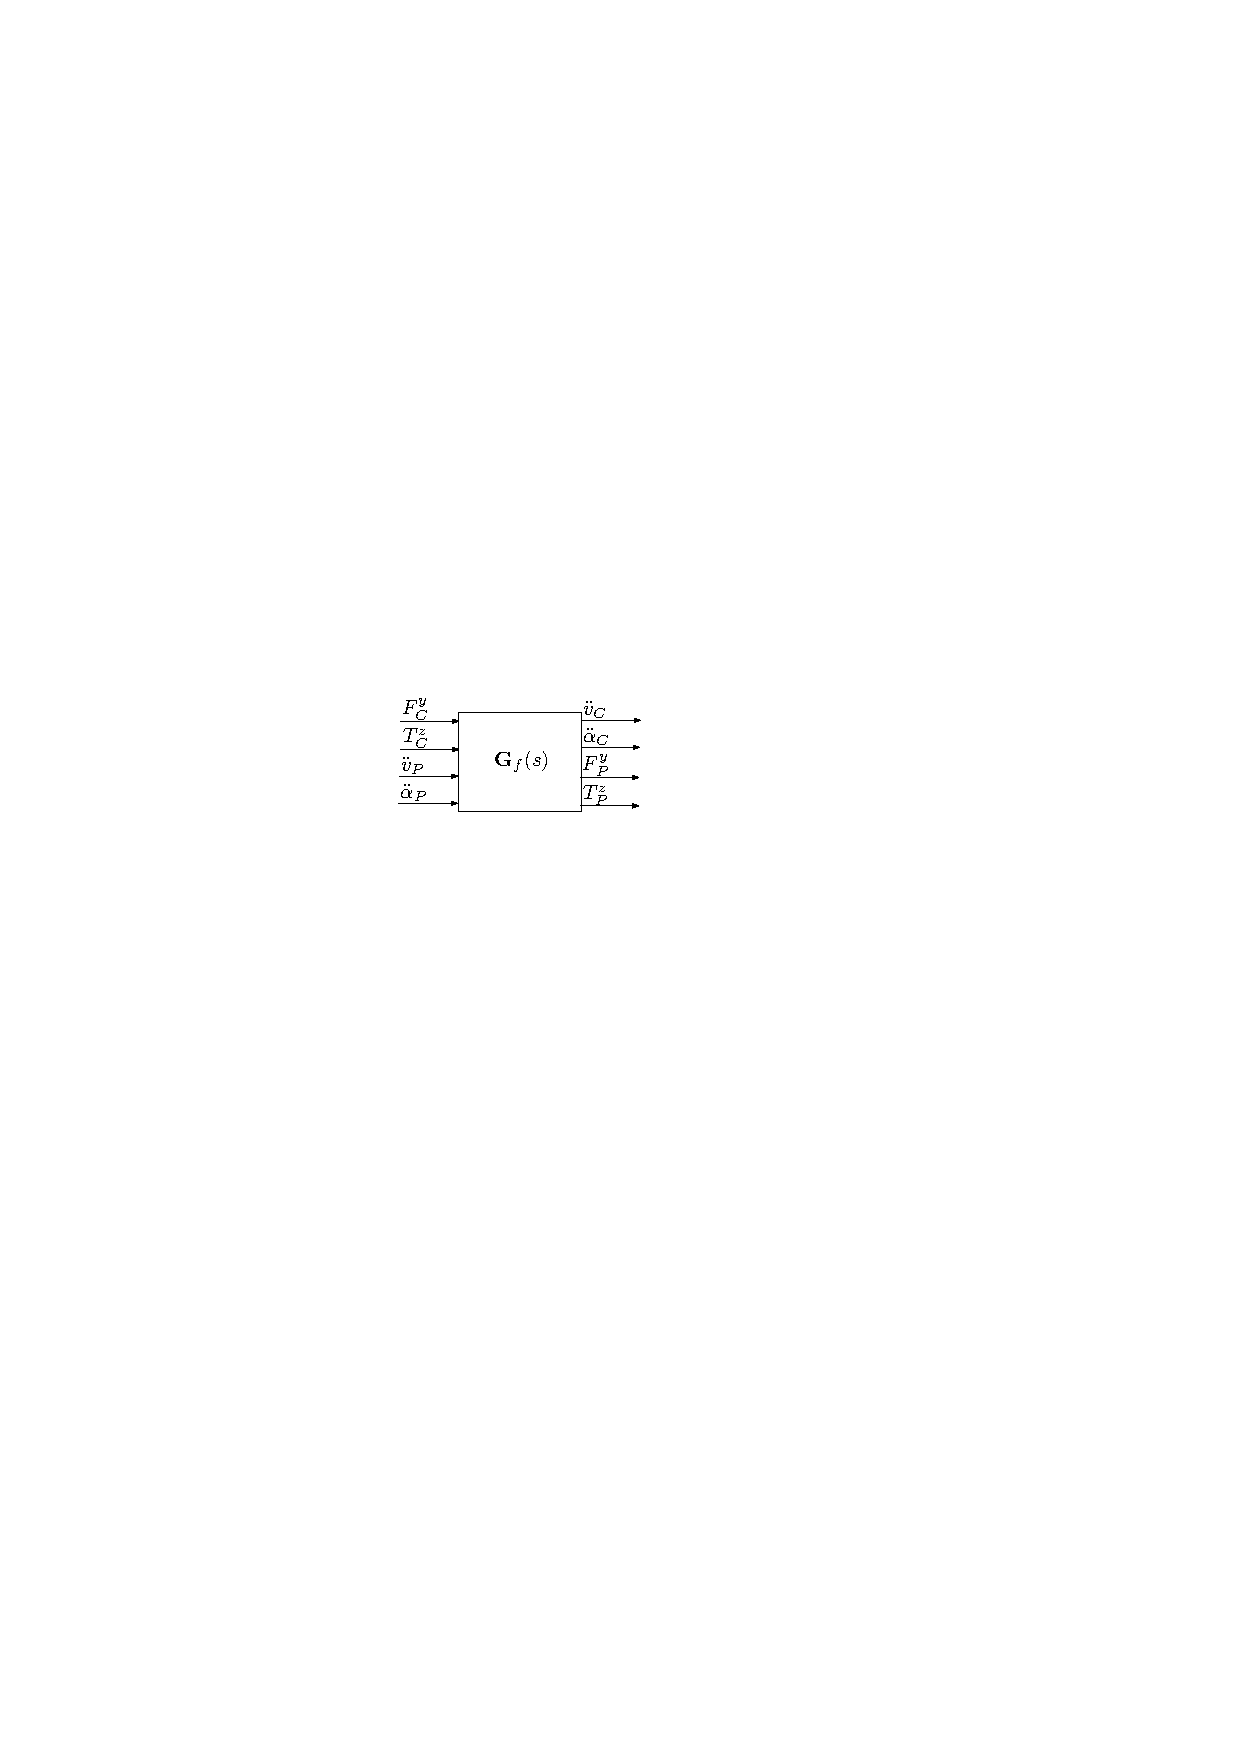
\includegraphics[width=0.3\textwidth]{TyRzb}
\caption{TITOP model $\mathbf{G}_{f}(s)$ block diagram of a flexible beam in bending.}
\label{fig:TyRz} 
\end{figure}

\subsubsection{Choice of the modal decomposition}
In this section the choice of the decomposition defined in equation (\ref{eq:decomp}) is discussed regarding the capability of the TITOP model $\mathbf{G}_{f}(s)$  (and its inverses) to take into account various boundary conditions. Among all possible boundary conditions, a very simple test consists in computing and comparing the natural frequencies $\omega_{cf,i}$ and $\omega_{fc,i}$ of models $\mathbf{G}_{f}(s)$ and $\mathbf{G}_{f}^{-1}(s)$, respectively. Indeed, $\mathbf{G}_{f}(s)$ is the model of the beam under the \textit{clamped-free} condition and $\mathbf{G}_{f}^{-1}(s)$ is the model of the beam under the \textit{free-clamped} condition. Since the beam is uniform, the natural frequencies of the 2 models must be equal: $\omega_{cf,i}=\omega_{fc,i},\;\forall\;i$.

Two decompositions are considered to build the TITOP model  $\mathbf{G}_{f}(s)$:
\begin{itemize}
\item the well-known clamped-free assumed mode decomposition \cite{MohanSahaMSD2007}. The model obtained from this decomposition is denoted $\mathbf{G}_{f,n}(s)$ where $n$ is the number of assumed modes.
\item the decomposition based on $5$-th order polynomial shape functions \cite{Murali2015}. The model obtained from this decomposition is denoted $\mathbf{G}_{f,pol}(s)$
\end{itemize}

\paragraph{Model $\mathbf{G}_{f,n}(s)$:} in that case, the decomposition is based on the $n$ first modes of the \textsc{Euler-Bernoulli} beam in the clamped-free condition and the shape functions in (\ref{eq:decomp}) are \cite{wiki,bishop1979mechanics}:
\begin{equation}\label{eq:phiref}
\phi_i(x)=\cos\beta_i x-\cosh\beta_i x-\frac{\cos\beta_i l+\cosh\beta_i l}{\sin\beta_i l+\sinh\beta_i l}(\sin\beta_i x-\sinh\beta_i x)
\end{equation}
where $\beta_i,\;i=1,\cdots,n$ are the $n$ first solutions of the  characteristic equation:\\ $\cos\beta l\cosh\beta l+1=0$. The natural frequencies are given by $\omega_{i,ref}=\beta_i^2\sqrt{\frac{E\,I_z}{\rho\,S}}$ and are the clamped-free reference values to evaluate approximate solutions. Such a decomposition basis is orthonormal and leads to $\mathbf{M}_{ff}=I_n$ and $\mathbf{K}=\mbox{diag}([\omega_{i,ref}^2])$. The value of $\mathbf{M}_{rf}$ and $\vec{\Phi}(l)$ are not detailed for sake of brevity.

\paragraph{Model $\mathbf{G}_{f,pol}(s)$:} in this approach given in more details in \cite{Murali2015}, the deflection $\widetilde{v}(x,t)$ in the moving frame $\widetilde{\mathcal{R}}$ is expressed as:
\[
\widetilde{v}(x,t)=a_2(t)x^2+a_3(t)x^3+a_4(t)x^4+a_5(t)x^5\,.
\]
This $5$-th order polynomial ensures that $\widetilde{v}(0,t)=\widetilde{v}'(0,t)=0,\;\forall\;t$. The coefficients $a_i(t)$ are then expressed as a function of $4$ time-domain functions $q_i(t)$ defined by:
\begin{equation}\label{eq:defq}
\vec{q}(t)=[\widetilde{v}''(0,t)\quad \widetilde{v}(l,t)\quad \widetilde{v}'(l,t)\quad \widetilde{v}''(l,t)]^T\;,
\end{equation}
and the shape functions vector reads:
\begin{equation}\label{eq:Phi}
  \vec{\phi}(x)=\left[\begin{array}{c}\frac{1}{2}x^2-\frac{3}{2l}x^3+\frac{3}{2l^2}x^4-\frac{1}{2l^3}x^5\\ \frac{10}{l^3}x^3-\frac{15}{l^4}x^4+\frac{6}{l^5}x^5\\
\frac{-4}{l^2}x^3+\frac{7}{l^3}x^4-\frac{3}{l^4}x^5\\
\frac{1}{2l}x^3-\frac{1}{l^2}x^4+\frac{1}{2l^3}x^5\end{array}\right]
\end{equation}
Data required to build the TITOP model $\mathbf{G}_{f,pol}(s)$ defined in equation (\ref{eq:Gfss}) are obtained using following decompositions:
\begin{equation}\label{eq:mass}
\left[\begin{array}{c|c}\mathbf{M}_{rr} & \mathbf{M}_{rf}^T \\\hline \mathbf{M}_{rf} & \mathbf{M}_{ff} \end{array}\right]=\frac{\rho S l}{55440}\left[\begin{array}{cc|cccc}
    55440 & 27720\,l &  462\,l^2 & 27720 & -5544\,l &  462\,l^2\\
         27720\,l& 18480\,l^2 &198\,l^3 &19800\,l &-3432\,l^2 &264\,l^3\\\hline
         462\,l^2 &198\,l^3&   6\,l^4 &  181\,l^2&  -52\,l^3&    5\,l^4\\
         27720&   19800\,l&   181\,l^2&  21720&  -3732\,l &  281\,l^2\\
         -5544\,l& -3432\,l^2& -52\,l^3 &-3732\,l& 832\,l^2 &  -69\,l^3\\
         462\,l^2 &264\,l^3  &  5\,l^4&  281\,l^2 &-69\,l^3  &   6\,l^4
 \end{array}\right]
\end{equation}
\begin{equation}\label{eq:raideur}
\mathbf{K}=\frac{EI_z}{70\,l^3}\left[\begin{array}{cccc}
            6\,l^4 & -30\,l^2 &8\,l^3  &    l^4\\
                -30\,l^2 & 1200  & -600\,l & 30\,l^2\\
                 8\,l^3& -600\,l& 384\,l^2& -22\,l^3\\
                 l^4  & 30\,l^2 &-22\,l^3   &6\,l^4 
\end{array}\right],\quad
\left[\begin{array}{c} \vec{\tau}^T\\ \hline \vec{\Phi}^T(l)
\end{array}\right]=
\left[\begin{array}{cc}
1 & 0 \\l & 0\\ \hline 0& 0\\ 1 &0 \\0 & 1\\ 0 & 0
\end{array}\right]\;.
\end{equation}
The clamped-free and free-clamped models obtained  from the TITOP models $\mathbf{G}_{f,pol}(s)$ and $\mathbf{G}_{f,n}(s)$ (for various number $n$ of assumed modes) are now evaluated in Table \ref{tab:datac} regarding the accuracy of the first two natural frequencies. Of course, the model $\mathbf{G}_{f,n}(s)$ provides the exact clamped-free frequencies for any values of $n$ since the clamped-free modes are exactly taken into account in this approach. But its inverse, which must represents the free-clamped model, is not accurate at all, even for high values of $n$ (for $n=16$, the order of the model $\mathbf{G}_{f,16}(s)$ is 32!!). In comparison, the model $\mathbf{G}_{f,pol}(s)$ is a $8$-th order model with only $4$ flexible modes which is quite accurate regarding the $2$ first natural frequencies from the clamped-free to free-clamped conditions.

In the following section, the TITOP model $\mathbf{G}_{f,pol}(s)$ is used to model an \textsc{Euler-Bernoulli} beam under the various well-known boundary conditions: free, clamped, support or sliding on each of the $2$ tips of the beam. In each case, the $2$ first natural frequencies are compared with the reference values provided by the beam theory.

\begin{table}[htbp!]
% table caption is above the table
\caption{Comparison of the first two frequencies of TITOP models and their inverses. The direct model corresponds to the clamped-free model of an \textsc{Euler-Bernoulli} beam. The inverse model corresponds to the free-clamped model. Frequencies are expressed using normalized units $\left(\sqrt{\frac{E\,I_z}{\rho\,S\,l^4}}\right)$.}
\label{tab:datac}       % Give a unique label
% For LaTeX tables use
\begin{tabular}{llllllll}
\hline\noalign{\smallskip}
  $i$ & $\omega_{i,ref}$ &  $\mathbf{G}_{f,pol}(s)$ &  $\mathbf{G}_{f,pol}^{-1}(s)$ &  $\mathbf{G}_{f,n}(s)$ &  $\mathbf{G}_{f,4}^{-1}(s)$  &  $\mathbf{G}_{f,8}^{-1}(s)$ &  $\mathbf{G}_{f,16}^{-1}(s)$ \\
\noalign{\smallskip}\hline\noalign{\smallskip}
$1$ & $3.5160$ & $3.5160$ & $3.5160$ & $3.5160\;\forall\,n$ & $4.4432$ & $3.9084$ & $3.7508$\\ 
$2$ & $22.034$ & $22.158$ & $22.158$ & $22.034\;\forall\,n$ & $27.486$ & $24.579$ & $23.585$\\ 
\hline
\end{tabular}
\end{table}

\subsubsection{Other boundary conditions}
The various classical (clamped, free, pinned, sliding) boundary conditions are taken into account by setting to $0$ the corresponding inputs of $\mathbf{G}_{f,pol}(s)$, or of its inversion around one or more channels. The procedure for such a channel inversion is described in appendix 1 under state-space formalism and can be directly applied to the TITOP model  $\mathbf{G}_{f,pol}(s)$ defined in equation (\ref{eq:Gfss}). Note that the $8$-component state vector $\vec{x}_f$ of $\mathbf{G}_{f,pol}(s)$ or of its various inverses has a physical meaning and is defined by:
\[
\vec{x}_f=\left[ \begin {array}{c} \vec{q}  \\ \dot{\vec{q}} \end{array}\right]\;,
\]
where more particularly (from (\ref{eq:defv}) and (\ref{eq:defq})):
\begin{eqnarray}\label{eq:xtyrz}
\vec{x}_f(2)&=& \vec{q}(2)= \widetilde{v}(l) = v_C-v_P-l\,\alpha_P\\ \nonumber
\vec{x}_f(3)&=& \vec{q}(3)= \widetilde{v}'(l)= \alpha_c-\alpha_P\;.
\end{eqnarray}
In the various cases presented in appendix 2, the channel inversion to be used on the TITOP model $\mathbf{G}_{f,pol}(s)$ in order to take into account the corresponding boundary conditions is detailed.  Some boundary conditions can introduce also some \textbf{internal state conditions} which can be used to reduce the order of the model. These conditions are also detailed in the various cases presented in appendix 2. The first two natural frequencies $\omega_i$, $i=1,2$ are then compared with the reference values $\omega_{i,ref}$ provided by beam theory \cite{bishop1979mechanics} in the same boundary conditions and the relative errors $\Delta \omega_i=100\,\frac{|\omega_i-\omega_i^{ref}|}{\omega_i^{ref}}$, $i=1,2$ are computed and summarized in Tables \ref{tab:Tff} to \ref{tab:Tss}.

Finally, one have to keep in mind that the model $\mathbf{G}_{f,pol}(s)$ and its various inverses describe the relationship between forces and accelerations. These models provide the frequencies of the flexible modes for various boundary conditions. To take into account the rigid modes that can appear in some cases (free-free, pinned-free, sliding-free, sliding-sliding), one have to consider the positions $v_P$, $\alpha_P$, $v_C$ and $\alpha_C$ as outputs of an augmented model. Of course, these positions can be obtained from accelerations using twice integrations, but it is recommended to use the internal state $\vec{x}_f$ and equations (\ref{eq:xtyrz}) to describe this augmented model by a minimal state-space representation. The block-diagram representation of this augmented model and the number of rigid modes are also detailed for the various cases presented in appendix 2.


In every case, the TITOP model $\mathbf{G}_{f,pol}(s)$ and its inverses provide a quite good approximation of the first two natural frequencies.

In conclusion, the polynomial approximation done in the TITOP model $\mathbf{G}_{f,pol}(s)$ leads to a simple analytical model (order $8$) which can be used during preliminary design phase. It allows varying conditions on a very large range, from clamped to free conditions for each translational or rotational d.o.f(s). The $5$-th order polynomial shape functions chosen to build the TITOP model allows the first two natural frequencies to be representative enough for arbitrary boundary conditions. The only task needed to vary these boundary conditions consists of the inversion of input/output channels of the TITOP model or the feedback of some dynamic model between its input and output ports. That will be illustrated in the  section \ref{sect:fb}. 

\subsubsection{Modal shapes of TITOP models }\label{sect:shape}
Let us consider the $8$-th order TITOP model of the beam  $\mathbf{G}_{f,pol}(s)$ or its inverses $\mathbf{G}_{f,pol}^{-1_{\mathbf{I}}}(s)$. For all these models, the state vector is still $\vec{x}_f(t)=[\vec{q}^T(t)\quad \dot{\vec{q}}^T(t)]^T$. 

Let $\mathbf{A}$, $\mathbf{B}$, $\mathbf{C}$ and $\mathbf{D}$ the 4 state-space matrices of one of these models, then the eigenvalue decomposition of $\mathbf{A}$ characterizes the free response of the model to initial conditions $\vec{x}_f(0)$ (i.e. when the inputs are set to $0$). The eigenvalues $\lambda_i$ of $\mathbf{A}$ are auto-conjugate pair associated to each natural frequencies ($\lambda_i=\pm j\,\omega_i$) of the $i$-th flexible mode ($i=1,\cdots,4$). The associated eigen-vector $\vec{v}_i$ represents the magnitude of the $i$-th mode on the components of the state vector $\vec{x}_f$:
\begin{equation}\label{eq:vf}
\vec{x}_f(t)=\left[\begin{array}{c} \vec{q}(t) \\ \dot{\vec{q}}(t)\end{array}\right]=\sum_{i=1}^4g_i\vec{v}_ie^{j(\omega_it+\varphi_i)}
\end{equation}
where the scalars $g_i$ and $\varphi_i$ depends on the initial conditions $\vec{x}_f(0)$. 

From equations (\ref{eq:defv}) and  (\ref{eq:decomp}), the deformation of the beam is:
\[
v(x,t)=[1\quad x \quad \vec{\phi}^T(x)]\left[\begin{array}{c} v_P(t) \\ \alpha_P(t) \\ \vec{q}(t)\end{array}\right]
\]
where $\vec{\phi}(x)$ is defined by (\ref{eq:Phi}). 

Modal shapes can be characterized by their contributions to the second time-derivative of the beam deflection $\ddot{v}(x,t)$ (which is proportional with  a factor $-\omega_i^2$ to the beam deflection $v(x,t)$). Indeed, let $\psi_i(x)$ be the modal shape of the $i$-th mode, then $v(x,t)$ can be decomposed as:
\[
v(x,t)=\sum_{i=1}^4g_i\psi_i(x)e^{j(\omega_it+\varphi_i)}
\]
and
\begin{equation}\label{eq:acc}
\ddot{v}(x,t)=-\sum_{i=1}^4g_i\omega_i^2\psi_i(x)e^{j(\omega_it+\varphi_i)}=[1\quad x \quad \vec{\phi}^T(x)]\left[\begin{array}{c} \ddot{v}_P(t) \\ \ddot{\alpha}_P(t) \\ \ddot{\vec{q}}(t)\end{array}\right]\;.
\end{equation}
$\ddot{\vec{q}}(t)$ can be decomposed using (\ref{eq:vf}) and the state matrix $\mathbf{A}$ (see appendix 1 for the submatrix notation):
\begin{equation}\label{eq:ms}
\ddot{\vec{q}}(t)=\sum_{i=1}^4g_i\mathbf{A}([5:8],:)\vec{v}_ie^{j(\omega_it+\varphi_i)}=-\sum_{i=1}^4g_i\omega_i^2\vec{v}_i([1:4)e^{j(\omega_it+\varphi_i)}\;.
\end{equation}
If the beam is clamped at $P$, then $\ddot{v}_P(t)= \ddot{\alpha}_P(t)=0$ and the identification of equation (\ref{eq:acc}) with (\ref{eq:ms}) gives:
\[
\psi_i(x)=-\vec{\phi}^T(x)\mathbf{A}([5:8],:)\vec{v}_i/\omega_i^2=\vec{\phi}^T(x)\vec{v}_i([1:4])\;.
\]
In the other cases, according to the channels (defined in the vector of indexes  $\mathbf{I}$) which are inverted in the model  $\mathbf{G}_{f,pol}^{-1_{\mathbf{I}}}(s)$, $\ddot{v}_P(t)$ and $\ddot{\alpha}_P(t)$ can be in the model outputs and their contribution to the modal shape $\psi_i(x)$ can be characterized using the matrix $\mathbf{C}$ of the model state-space representation. In a general way, one can define:
\begin{eqnarray}\nonumber
\mathbf{C}_{v_P}&=&\mathbf{C}(3,:)\quad\mbox{if}\quad 3\in\mathbf{I}\;;\quad \mathbf{C}_{v_P}=\mathbf{0}_{1\times 8}\quad\mbox{otherwise}\;,\\\nonumber
\mathbf{C}_{\alpha_P}&=&\mathbf{C}(4,:)\quad\mbox{if}\quad 4\in\mathbf{I}\;;\quad \mathbf{C}_{\alpha_P}=\mathbf{0}_{1\times 8}\quad\mbox{otherwise}\;,
\end{eqnarray}
then, 
\begin{equation}\label{eq:psi}
\psi_i(x)=-[1\quad x \quad \vec{\phi}^T(x)]\left[\begin{array}{c}\mathbf{C}_{v_P}\\ \mathbf{C}_{\alpha_P} \\\mathbf{A}([5:8],:)\end{array}\right]\vec{v}_i/\omega_i^2\;.
\end{equation}

Thus, the modal shapes for arbitrary boundary conditions can be easily characterized from the eigenvectors / eigenvalues decomposition of the TITOP model or its inverses. As an example, the modal shapes $\psi_1(x)$ and $\psi_2(x)$ of the first two modes of the free-clamped beam modeled by $\mathbf{G}_{f,pol}^{-1_{[1:4]}}(s)$ are depicted in Fig. \ref{fig:fc1_2} and compared with the reference modal shapes $\phi_1(x)$ and $\phi_2(x)$ provided by equation (\ref{eq:phiref}) by changing $x$ by $l-x$. One can appreciate the accuracy of the first two modal shapes provided by the TITOP model.
\begin{figure}[htbp!]
  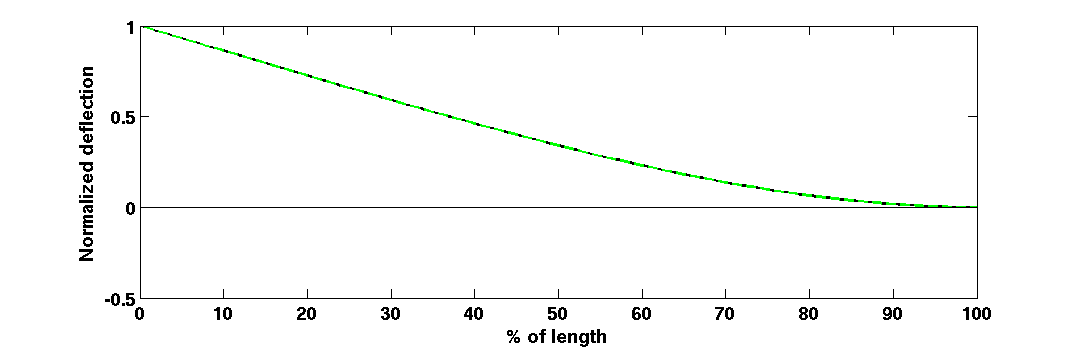
\includegraphics[width=\textwidth]{fc_mode1}\\
  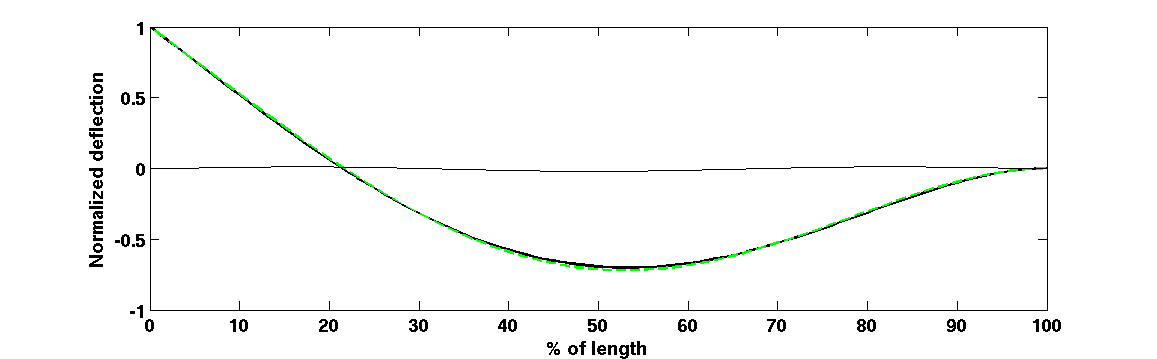
\includegraphics[width=\textwidth]{fc_mode2}
\caption{Modal shapes of the first (top) and second (bottom) free-clamped modes: $\psi_i(x)$ (solid bold), reference $\phi_i(x)$ (dashed) and error $\phi_i(x)-\psi_i(x)$ (solid).}
\label{fig:fc1_2} 
\end{figure}

\subsection{Pure traction along $(P^0,\vec{x})$-axis}
Only one flexible mode is considered to represent the traction-compression along  $(P^0,\vec{x})$-axis. Let $u(x,t)$ the axial deformation at any point of abscissa  $x$ ($x\in [0\,;\;\; l]$) due to axial forces $-F^x_P$ and $F^x_C$ applied to the beam at points $P$ and $C$, respectively. Then, it is assumed that:
\[
u(x,t)= u_P(t)+\frac{x}{l}(u_C(t)-u_P(t))=u_P(t)+\frac{x}{l}\,\delta_u(t)=\left[1\quad \frac{x}{l}\right]\left[\begin{array}{c} u_P(t)\\ \delta_u(t)\end{array}\right]\,,
\]
that is, the deformation at $x$ is proportional to the total deformation $\delta_u(t)$ of the beam.

Then, the kinetic energy reads:
\[
\mathcal{T}_x=\frac{1}{2}\int_{0}^l\rho\,S\,\left(\frac{\partial u}{\partial t}(x,t)\right)^2 \,dx=\frac{1}{2}[\dot{u}_P \quad \dot{\delta}_u]\mathbf{M}_x\left[\begin{array}{c}\dot{u}_P \\ \dot{\delta}_u \end{array}\right]
\]
with: $\mathbf{M}_x=\rho S l\left[\begin{array}{cc}1 & 1/2 \\ 1/2 & 1/3 \end{array}\right]$,
and the potential energy reads:
\[
\mathcal{V}_x=\frac{1}{2}\int_{0}^lE\,S\,\left(\frac{\partial u}{\partial x}(x,t)\right)^2 \,dx=\frac{1}{2}[u_p \quad \delta_u]\mathbf{K}_x\left[\begin{array}{c}u_p \\ \delta_u \end{array}\right]
\]
with: $\mathbf{K}_x=\frac{E S}{l}\left[\begin{array}{cc}0 & 0 \\ 0 & 1 \end{array}\right]$.

The TITOP model $\mathbf{G}_t(s)$ relative to the traction/compression dynamics along $(P^0,\vec{x})$-axis is:
\begin{equation} \label{eq:Gtss}
\left[\begin{array}{c} \dot{\delta}_u \\ \ddot{\delta}_u\\ \hline
\ddot{u}_C
 \\ 
F^x_P
 \end{array}\right]=\left[\begin{array}{cc|cc}
0 & 1 & 0 & 0\\ -\frac{3\,E}{\rho\,l^2} & 0 & \frac{3}{\rho\,S\,l} & -\frac{3}{2}\\ \hline -\frac{3\,E}{\rho\,l^2} & 0 & \frac{3}{\rho\,S\,l}  & -\frac{1}{2} \\ \frac{3\,E\,S}{2\,l} & 0 &  -\frac{1}{2} & -\frac{\rho\,S\,l}{4}\end{array}\right]\left[\begin{array}{c} \delta_u \\ \dot{\delta}_u \\ \hline  
F^x_C
\\ 
\ddot{u}_P
 \end{array}\right]
% =\left[\begin{array}{c|c}
%  A_{Tx} & B_{Tx} \\ \hline C_{Tx} & D_{Tx}
% \end{array}\right]
% \left[\begin{array}{c} \delta u \\ \dot{\delta u} \\ \hline  
% F^x_C
% \\ 
% \ddot{u}_P
%  \end{array}\right]
\;.
\end{equation}
\subsection{Two-port model $\mathbf{G}(s)$ of a beam in the planar case}
From equations (\ref{eq:Gfss}) and (\ref{eq:Gtss}), the $6\times 6$ $10$-th order TITOP model $\mathbf{G}(s)$ of the beam in the plane $(P^0,\mathbf{x},\mathbf{y})$ reads:
\begin{equation}\label{eq:Gss}
\mathbf{G}(s)=\mathbf{T}\,\left[\begin{array}{cc}\mathbf{G}_f(s) & \mathbf{0}_{4\times 2}\\\mathbf{0}_{2\times 4}& \mathbf{G}_t(s) \end{array}\right]\,\mathbf{T}^T
\end{equation}
where the permutation matrix $\mathbf{T}$ is
\[
\mathbf{T}=\left[\begin{array}{cccccc}
0 & 0 & 0 & 1 & 0 & 0\\ 1 & 0 & 0 & 0 & 0 & 0\\
0 & 1 & 0 & 0 & 0 & 0\\ 0 & 0 & 0 & 0 & 0 & 1\\
0 & 0 & 1 & 0 & 0 & 0\\ 0 & 0 & 0 & 1 & 0 & 0
\end{array}\right]\;.
\]
The block-diagram of $\mathbf{G}(s)$ is depicted in Fig. \ref{fig:G}.
\begin{figure}[htbp!]
  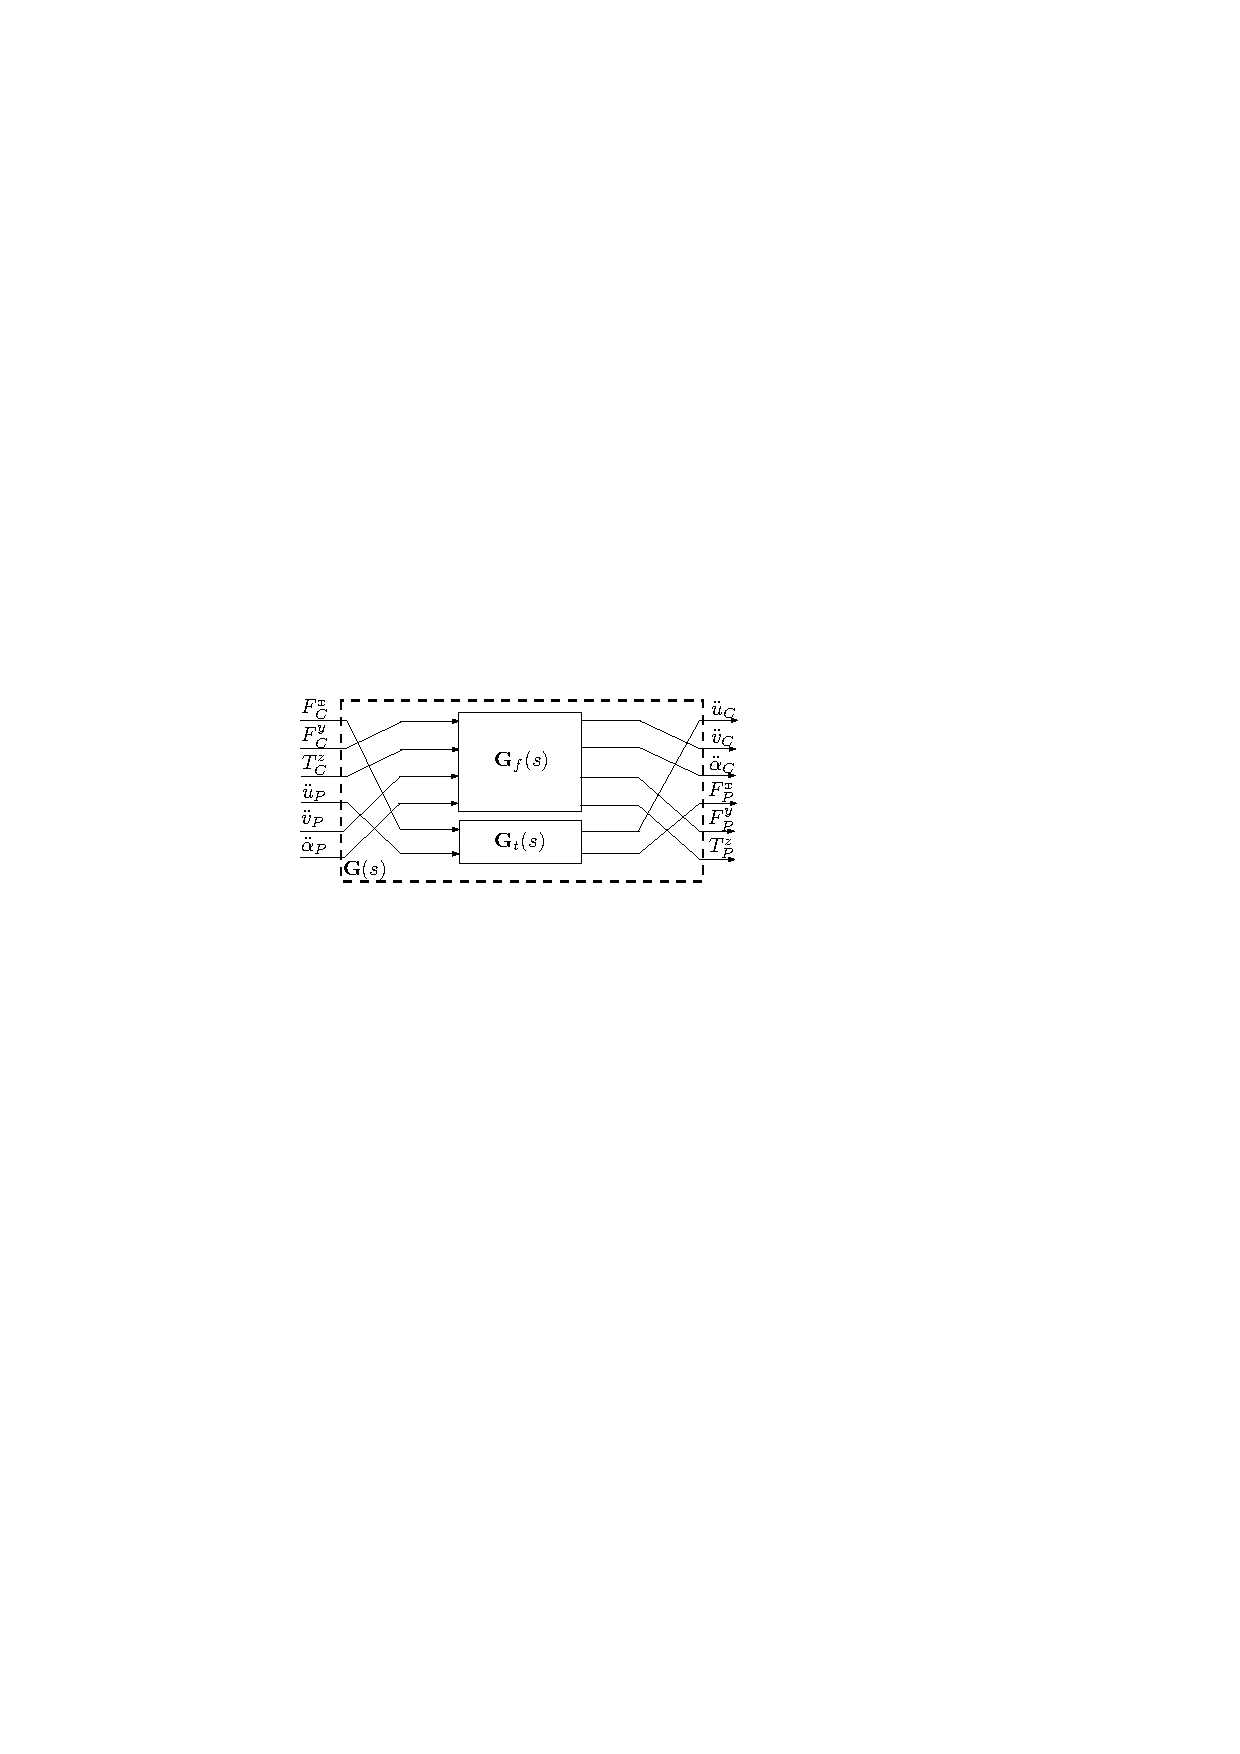
\includegraphics[width=0.5\textwidth]{Gb}
\caption{TITOP model $\mathbf{G}(s)$ block diagram.}
\label{fig:G} 
\end{figure}

In \cite{Murali2015}, the TITOP model of a uniform beam in detailed in the $3$-dimension case). This parametric model is then used to model and design a boom linking a flexible deployable antenna to a flexible spacecraft.

\section{Illustration: planar flexible four bar mechanism}\label{sect:fb}
In this section, the two-input two-output model approach presented in the previous section is applied to the well-known four bar mechanism depicted in Fig. \ref{fig:4bars}, taking into account the flexibility in the crank, in the coupler and in the follower. This mechanism is a closed-loop kinematic chain with one rigid degree-of-freedom and was largely studied in past decades \cite{Kitis1990267},  \cite{shigley1980}, \cite{Turcic1984} and more recently \cite{Sitti2003} to design efficient vibrating actuator. The objective is to compute the linear model $\mathbf{G}_{4\,bars}(s,\theta_1)$ between the torque $T^z_{P_1}$  applied on the crank at point $P_1$ and the angular acceleration of the crank $\ddot{\alpha}_{P_1}=\delta\ddot{\theta}_1$ for a given angular configuration $\theta_1$. First natural frequencies and modal shapes of the mechanism are then analyzed with respect to the crank angle $\theta_1$. The numerical values are taken from  \cite{Kitis1990267} (translated in the International System of Units) for result comparison and summarized in Table \ref{tab:data}.
The corresponding natural frequencies are then called free frequencies (and denoted $\omega_f(i)$) since the crank is free to rotate around $(P_1,\vec{z}_1)$ axis. The modeling approach provides also the cantilevered frequencies  $\omega_c(i)$, i.e. when the crank is clamped on the ground, which are easily computed by considering the inverse model $\mathbf{G}_{4\,bars}^{-1}(s,\theta_1)$.

\begin{figure}[htbp!]
  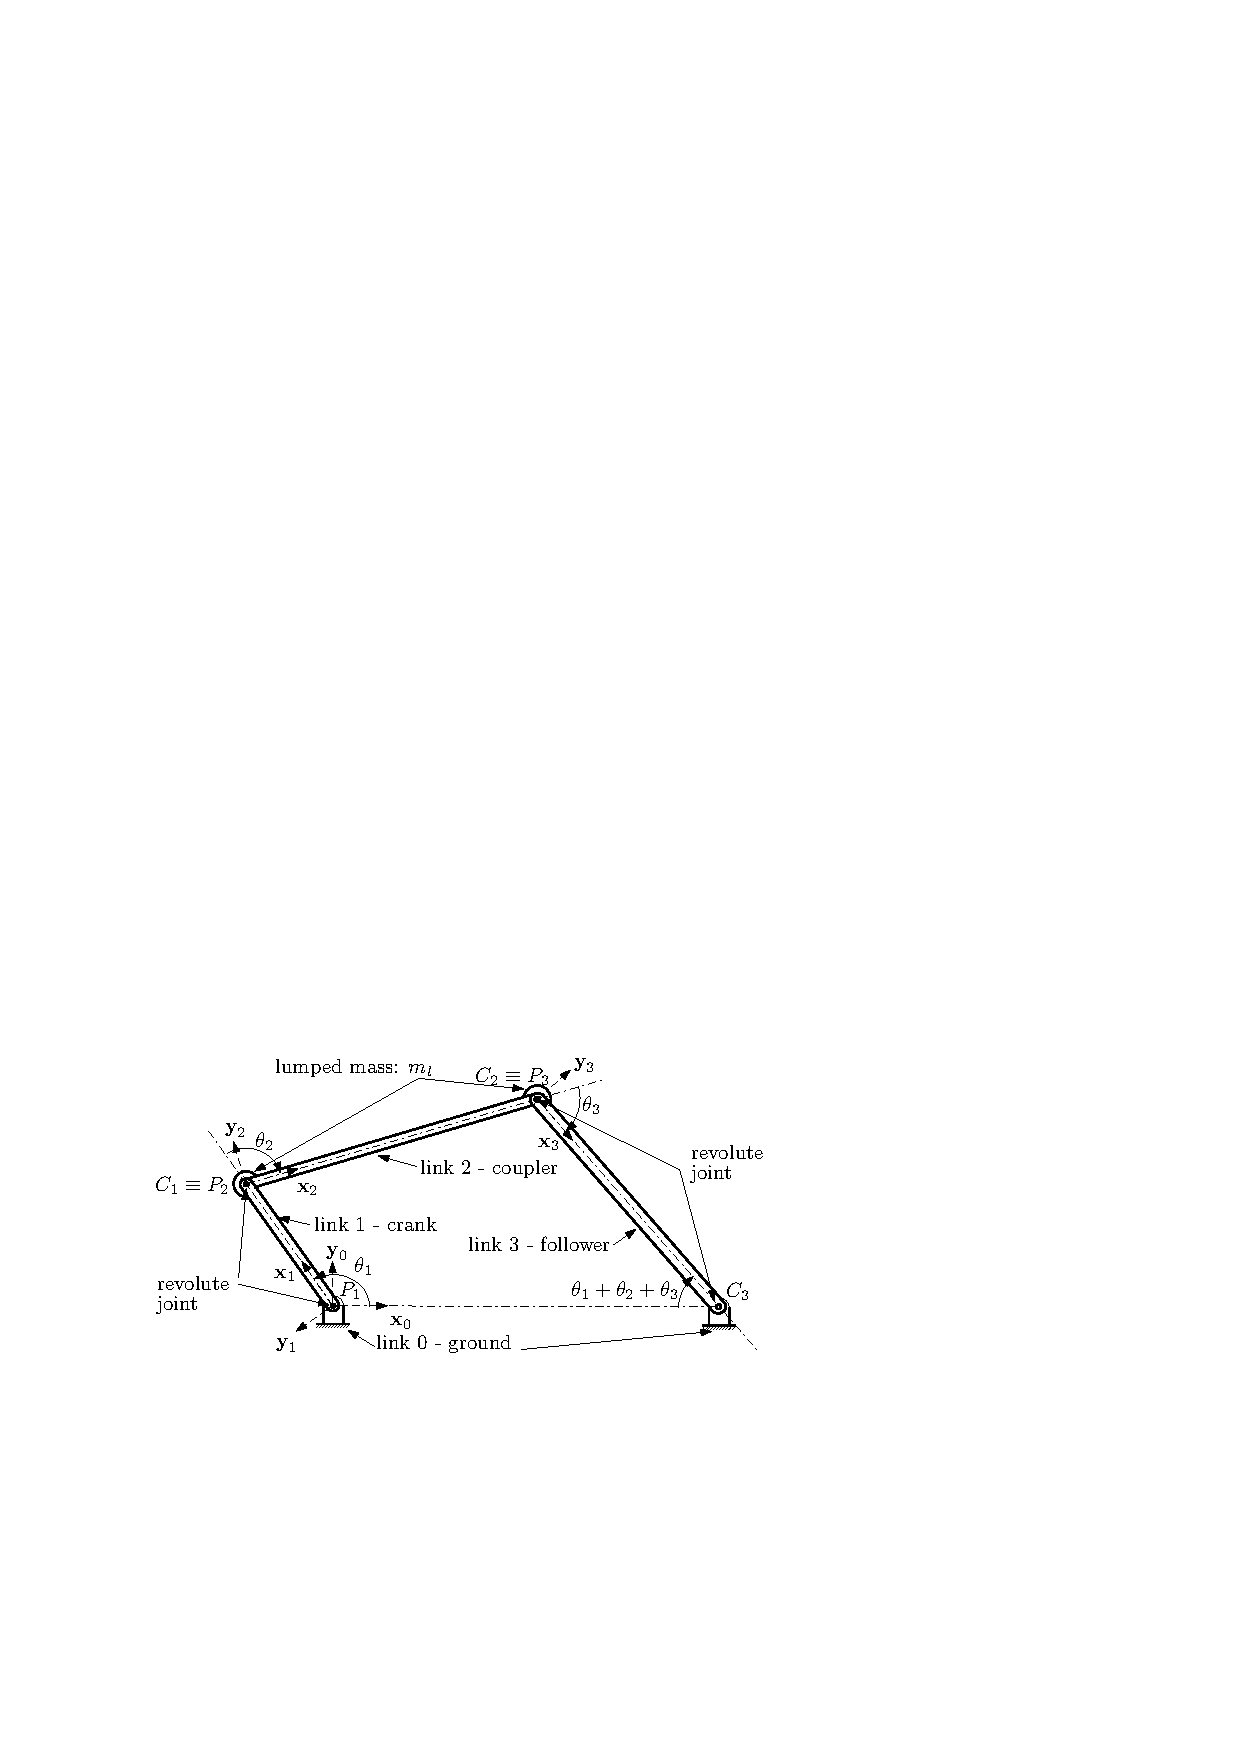
\includegraphics[width=0.7\textwidth]{fourbars}
\caption{Four-bar mechanism.}
\label{fig:4bars} 
\end{figure}

\begin{table}[htbp!]
% table caption is above the table
\caption{Four-bar mechanism links properties}
\label{tab:data}       % Give a unique label
% For LaTeX tables use
\begin{tabular}{lllll}
\hline\noalign{\smallskip}
  $i$ & $0$ &  $1$ &  $2$ &  $3$  \\
\noalign{\smallskip}\hline\noalign{\smallskip}
Name & ground & crank & coupler & follower \\ 
Length $l_i\,(m)$ & $0.254$ & $0.108$ & $0.2794$ & $0.2705$\\
Cross section $S_i\,(m^2)$ & $-$ & $1.0774\,10^{-4}$ & $4.0645\,10^{-5}$ & $4.0645\,10^{-5}$ \\
Flexural rigidity $(EI)_i\,(Nm^2)$ & $-$ & $11.472$ & $0.616$ & $0.616$ \\
\hline
\end{tabular}
Each link is a uniform beam with a mass density $\rho=2714\,Kg/m^3$ and a modulus of elasticity $E=7.1\,10^{10}\,N/m^2$. The lumped masses of bearing assemblies in revolute joints between link 2 and link 3 and between link 3 and link 4 are equal: $m_l=0.042\,kg$.
\end{table}

From data of Table \ref{tab:data}, TITOP models of the crank $\mathbf{G}_1(s)$, the coupler  $\mathbf{G}_2(s)$ and the follower  $\mathbf{G}_3(s)$ can be built from equations (\ref{eq:Gfss}), (\ref{eq:mass}), (\ref{eq:raideur}), (\ref{eq:Gtss}) and (\ref{eq:Gss}).  The ground ($i=0$ or $4$) is assumed to be rigid. 
The planar wrenches and acceleration twists on the inputs and outputs of each model $\mathbf{G}_i(s)$ are expressed in the body frame $\mathcal{R}_i$.  Considering the linear model around a given angular configuration (small variations), all the frames $\mathcal{R}_i$ are assumed to be inertial frames. For a given crank angle $\theta_1$, two kinematic constraints hold:
\begin{eqnarray}\nonumber
l_1 \cos{\theta_1}+l_2 \cos{(\theta_1+\theta_2)}+l_3 \cos{(\theta_1+\theta_2+\theta_3)}&=&l_0 \\ \nonumber
l_1 \sin{\theta_1}+l_2 \sin{(\theta_1+\theta_2)}+l_3 \sin{(\theta_1+\theta_2+\theta_3)}&=&0\;.
\end{eqnarray}
They are solved in $\theta_2$ and $\theta_3$ using the equations given by \textsc{Shigley} and \textsc{Uicker} \cite{shigley1980}. The values of $\theta_i$, $i=1,2,3$, allow the (planar) direction cosine matrices between the various frames  $\mathcal{R}_i$ to be computed:
\[
\mathbf{P}_{i/i-1}=\left[\begin{array}{cc}\cos{\theta}_i & -\sin{\theta_i} \\ \sin{\theta_i} & \cos{\theta_i}\end{array}\right]
\]

The revolute joints between the links enforce geometrical constraints between inputs and outputs of models $\mathbf{G}_i(s)$:
\[
P_{i}\equiv C_{i-1}\quad \Rightarrow \quad  \left[\begin{array}{c}\ddot{u}_{P_i} \\ \ddot{v}_{P_i}\end{array}\right]=\mathbf{P}_{i/i-1}^T\left[\begin{array}{c}\ddot{u}_{C_{i-1}} \\ \ddot{v}_{C_{i-1}}\end{array}\right]
\]
Some dynamic boundary conditions also hold on the inputs of the 3 models using channel(s) inversion if required:
\begin{itemize}
\item for the crank ($i=1$) and the coupler ($i=2$), the inputs of the model $i$ must take into account that: (i) $F^x_{C_i}$ and $F^y_{C_i}$ are constrained by the contact force applied by the link $i+1$ and the inertial force of the lumped mass:\begin{equation}
\left[\begin{array}{c}F^x_{C_{i}} \\ F^y_{C_{i}}\end{array}\right]=\mathbf{P}_{i+1/i}\left[\begin{array}{c} F^x_{P_{i+1}} \\ F^y_{P_{i+1}}\end{array}\right]-m_l\left[\begin{array}{c}\ddot{u}_{C_{i}} \\ \ddot{v}_{C_{i}}\end{array}\right]\;,
\end{equation} (ii) $T^z_{C_i}=0$ due to the revolute joint (no torque can be applied though the passive revolute joint),  (iii) $-T^z_{P_i}$ is equal to the torque $u$ applied by the driven system (crank case) or $T^z_{P_i}=0$ if the revolute joint is free (coupler case). Thus $T^z_{P_i}$ must be on the input and the model to be used for the crank and the coupler are $\mathbf{G}_1^{-1_6}(s)$ and $\mathbf{G}_2^{-1_6}(s)$, respectively,
\item for the follower ($i=3$): the same condition on $T^z_{P_3}$ appears but it is necessary to invert the first two channels of $\mathbf{G}_3(s)$ in order to close the kinematic loop, and to impose that $\ddot{u}_{C_3}$ and $\ddot{v}_{C_3}$ are zero due to the revolute joint on ground. Then, the model to be used for the follower is $\mathbf{G}_3^{-1_{[1,2,6]}}(s)$ and the first two outputs are the forces $F^x_{C_3}$ $F^y_{C_3}$ applied by the follower on the ground.
\end{itemize}
All these geometrical and dynamical boundary conditions can be easily expressed using the block diagram model depicted in Fig. \ref{fig:4bsch}. From this block diagram representation, the model  $\mathbf{G}_{4\,bars}(s,\theta_1)$ between the torque $u$ applied to the crank and the crank acceleration $y=\ddot{\alpha}_{P_1}$ can then be easily derived using \matlab/ \simulink and the function \verb|linmod|. The modal analysis of this model provides the free pulsations $\omega_f(i)$ of the mechanism. Note that the order of $\mathbf{G}_{4\,bars}(s,\theta_1)$ is $30$: this model includes $15$ flexible modes ($5$ modes per link with $4$ modes for bending in the plane ($P_i,\vec{y}_i,\vec{z_i}$) and $1$ mode for traction-compression along ($P_i,\vec{x}_i$)-axis). But this model does not include the rigid mode  of the mechanism. For control design purpose, this rigid mode can be included augmenting the model by a double integration:
\[
\frac{\alpha_{p_1}}{u}(s,\theta_1)=\mathbf{G}_{4\,bars}(s,\theta_1)\;\frac{1}{s^2}\;.
\]

\begin{figure}[htbp!]
  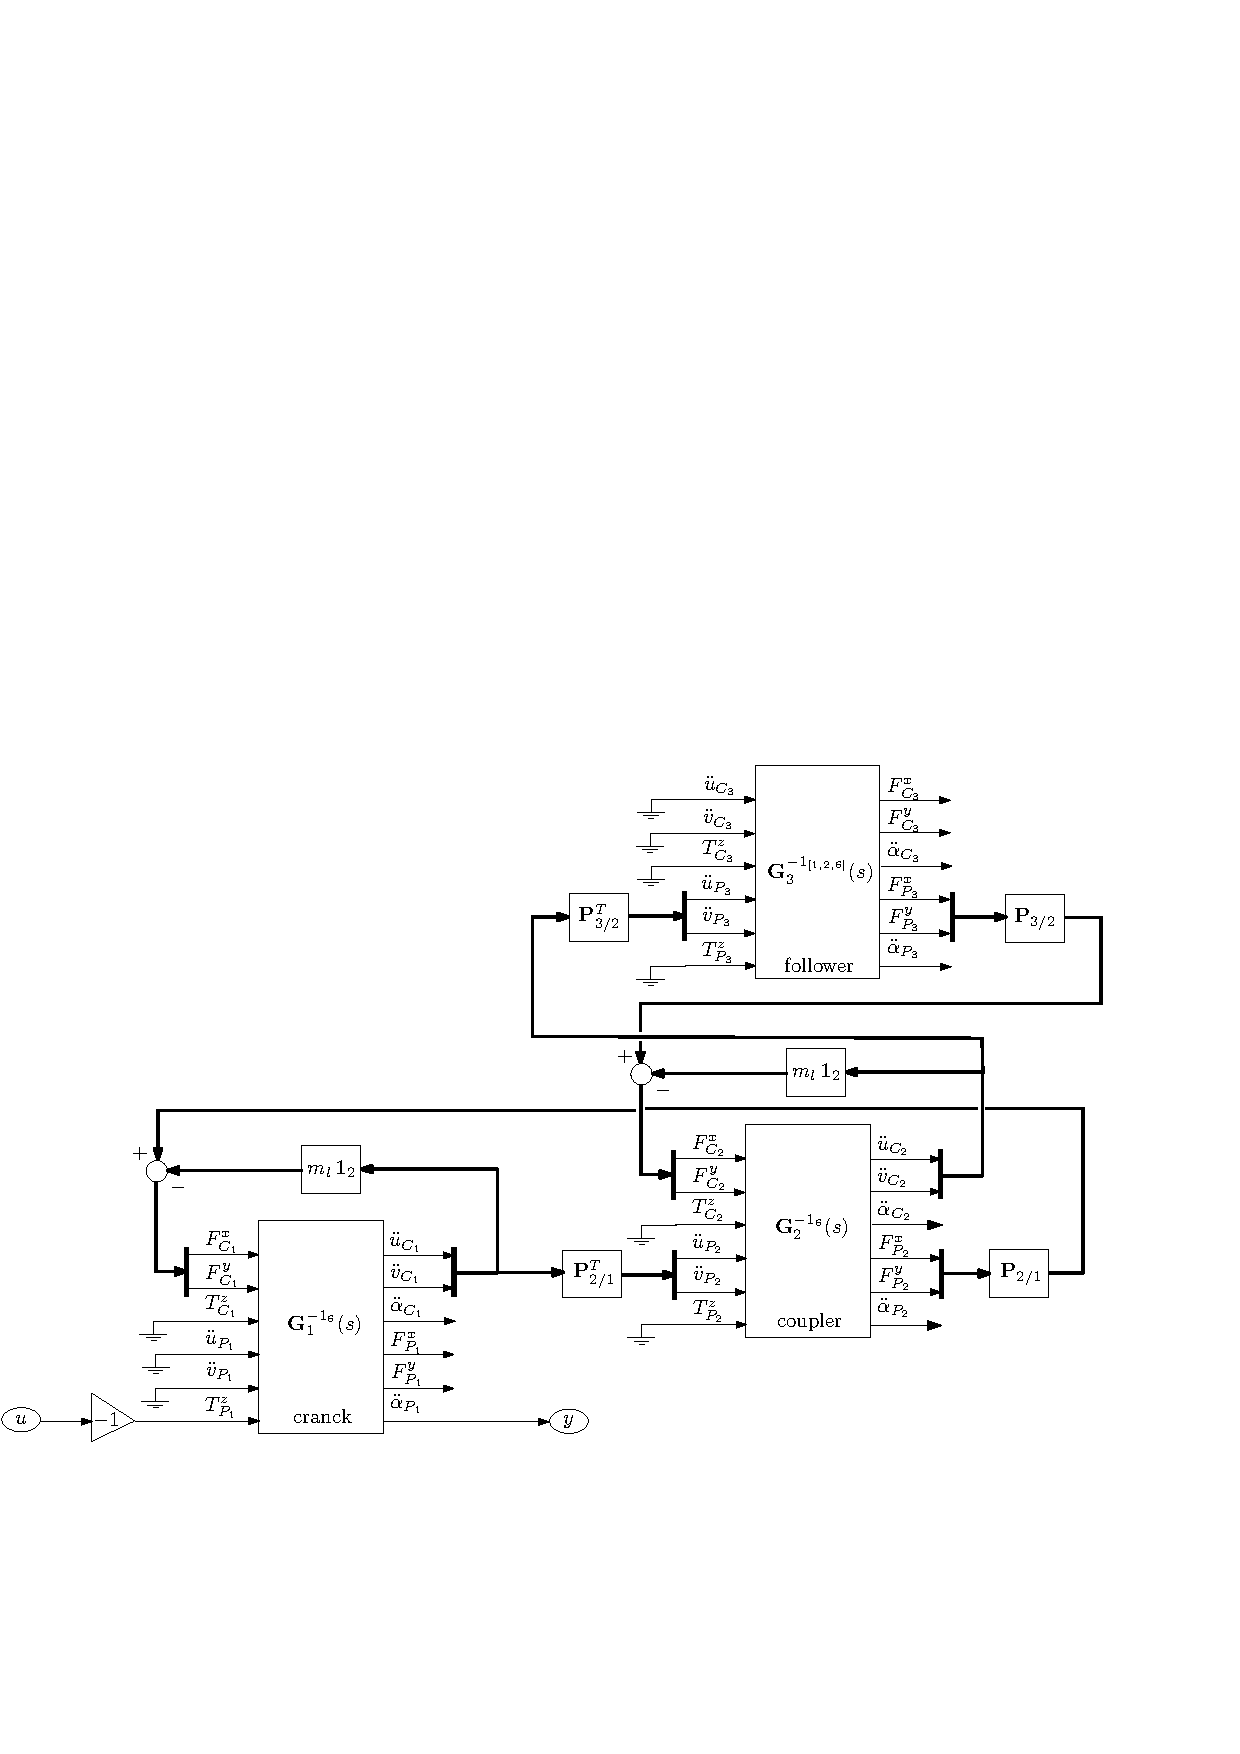
\includegraphics[width=1\textwidth]{fbschemab}
\caption{Block-diagram of model $\mathbf{G}_{4\,bars}(s,\theta_1)$ between the crank torque $u$ and the crank acceleration $y=\ddot{\alpha}_{P_1}$.}
\label{fig:4bsch} 
\end{figure}

To evaluate the accuracy of this model, the cantilevered pulsations $\omega_c(i)$ are computed from the inverse model $\mathbf{G}_{4\,bars}^{-1}(s,\theta_1)$ and compared with the results already published on the same mechanism \cite{Kitis1990267}, \cite{Turcic1984}. The first, second and third cantilevered frequencies are plotted in Fig. \ref{fig:modes123} versus crank angle. The modal shapes of the mechanism computed from the accelerations (see section \ref{sect:shape}) of the first 3 modes for two crank angle configurations ($0$ and $180^{\circ}$) are plotted in Fig. \ref{fig:shapes0} and \ref{fig:shapes180}. One can see that these results fit exactly the ones presented in \cite{Kitis1990267}.
\begin{figure}[htbp!]
  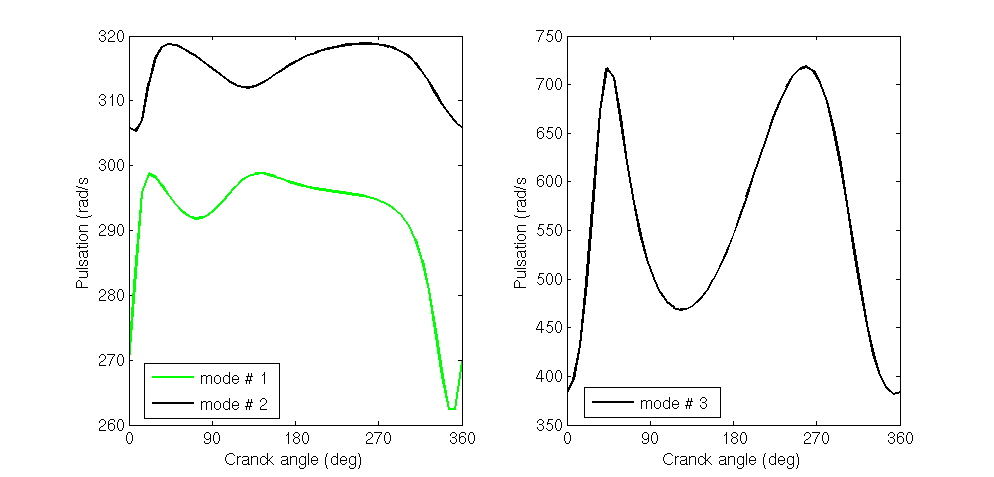
\includegraphics[width=1\textwidth]{modes123}
\caption{$\omega_{c}(i)\;i=1,2,3$ versus crank angle $\theta_1$.}
\label{fig:modes123} 
\end{figure}
\begin{figure}[htbp!]
  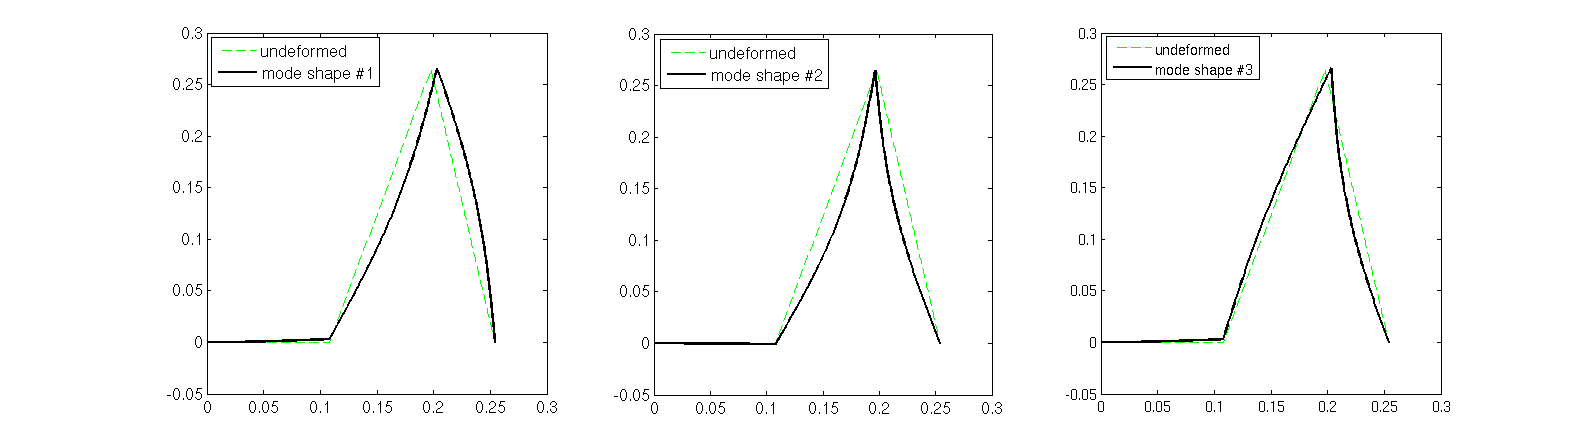
\includegraphics[width=1\textwidth]{shapes0}
\caption{First three modal shapes for crank angle $\theta_1=0$.}
\label{fig:shapes0} 
\end{figure}
\begin{figure}[htbp!]
  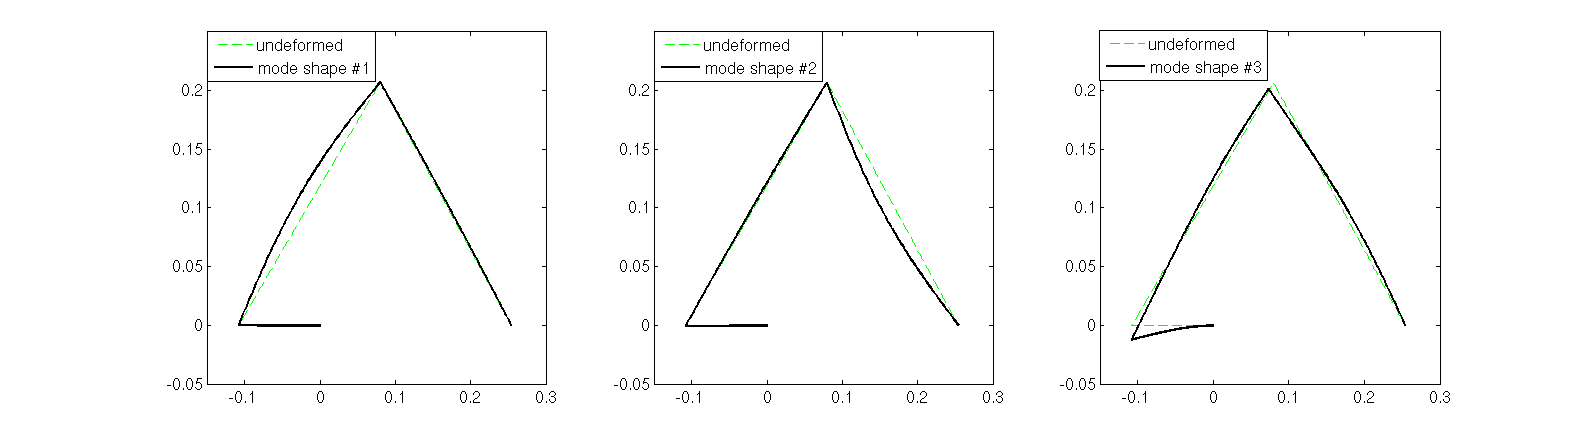
\includegraphics[width=1\textwidth]{shapes180}
\caption{First three modal shapes for crank angle $\theta_1=180\,deg$.}
\label{fig:shapes180} 
\end{figure}

\section{Conclusions}
The objective of this paper is to present the interest of the Two-Input Two-Output Ports approach to model any kind of flexible multibody systems. The novelty lies in the manipulation of transfer between accelerations and forces and to embed, in the same minimal state-space representation, the direct dynamic model of a body seen from one point and the inverse dynamic model seen from another point. All channels of this transfer are invertible allowing to consider arbitrary boundary conditions at these points. By comparison with the \textsc{Newton}-\textsc{Euler} method, commonly used to model multibody system dynamics, the forward and backward recursions are directly solved by the feedback connections between the inputs and the outputs of the TITOP models of each body. Such a dynamic model is today restricted to the linear behavior of the multibody system and to loads lumped at some particular points of the structure. The methodological utility of this approach has been highlighted on the flexible four bar mechanism. 

Further works need to be performed to extend this approach to aeronautical engineering, more particularly to take into account distributed loads along each body of the system and non-linear effects which could appear when the rate of variation of the configuration parameters is determinant. In this current state, this approach is fully applicable to space applications (large flexible orbital structures) but the proposed extensions are still required to apply it to helicopter rotor dynamic model, for instance.

%\nocite{PEREZ2015275,Perez2015}
\section*{Appendix 1: matrix and linear system operations}\label{sect:annexe}
Basic operations on matrices and linear dynamic systems and finally the inversion of one (or more) input-output channel(s) in a linear system are presented in this section.

Let us consider a square (same number of inputs and outputs) linear system $\mathbf{G}(s)$ ($s$ stands for the \textsc{Laplace} variable) with order $n$ and $m$ channels (i.e. $m$ inputs and $m$ outputs). A state-space realization of the system $\mathbf{G}(s)$ is a set of 4 matrices $\mathbf{A}_{n \times n}$, $\mathbf{B}_{n \times m}$, $\mathbf{C}_{m \times n}$, $\mathbf{D}_{m \times m}$ such that:
\begin{equation}
\mathbf{G}(s)=\mathbf{D}+\mathbf{C}\left( s\mathbf{I}_n-\mathbf{A}\right)^{-1}\mathbf{B}\quad \mbox{also noted:}\quad \mathbf{G}(s)\equiv \left[\begin{array}{c|c}\mathbf{A} & \mathbf{B} \\ \hline \mathbf{C} & \mathbf{D} \end{array}\right]\;.
\end{equation}

\paragraph{Submatrices and subsystems:} \matlab  nomenclature is used to define the submatrix $\mathbf{M}(\mathbf{I},\mathbf{J})$ (resp. subsystem $\mathbf{G}_{\mathbf{I},\mathbf{J}}(s)$) restricted to the rows (resp. outputs) and the columns (resp. inputs) ordered in vectors of indices $\mathbf{I}$ and $\mathbf{J}$. 
%submatrix of a matrix $\mathbf{M}$ restricted to the rows defined and ordered in the vector of indices $\mathbf{I}$, and to the columns defined  and ordered in the vector of indices $\mathbf{J}$ is denoted $\mathbf{M}(\mathbf{I},\mathbf{J})$ or, for brevity, $\mathbf{M}_{\mathbf{I},\mathbf{J}}$.\\ For example, if $\mathbf{M}=\left[\begin{array}{cc} 0.1 & 0.2 \\0.3 & 0.4 \end{array}\right]$ then $\mathbf{M}(2,[2,\;1])=\left[\begin{array}{cc} 0.4 & 0.3 \end{array}\right]$.\\
%The columns (resp. rows) of $\mathbf{M}$ defined and ordered in the vector of indices $\mathbf{J}$ (resp. $\mathbf{I}$) are denoted $\mathbf{M}(:,\mathbf{J})$ (resp. $\mathbf{M}(\mathbf{I},:)$). Finally, let $i$ and $j>i$ two integers, then 
%$\mathbf{I}=[i:j]$ is the vector of indices from $i$ to $j$.
%
%The same notation is used to define the subsystem $\mathbf{G}_{\mathbf{I},\mathbf{J}}(s)$ of a system $\mathbf{G}(s)$ between the outputs defined and ordered in the vector of indices $\mathbf{I}$ and the inputs defined and ordered in the vector of indices $\mathbf{J}$.

\paragraph{Single channel inversion:} the system corresponding to the inversion of the $i$-th channel of the system $\mathbf{G}(s)$ ($i\in[1,\,m]$) is denoted $\mathbf{G}^{-1_i}(s)$ and can be characterized by the following state-space realization (equation (\ref{eq:ginv})).\\
Let $\mathbf{J}$ be the vector of indices form $1$ to $m$ without $i$: $\mathbf{J}=[1,\cdots,i-1,i+1,\cdots,m]$. It is assumed that $\mathbf{D}(i,i)\neq 0$. Then let us denote $f_i=\frac{1}{\mathbf{D}(i,i)}$  and define:
\[
\widetilde{\mathbf{G}}^{-1_i}(s) \equiv \left[\begin{array}{c|c}\mathbf{A}-f_i\mathbf{B}(:,i)\mathbf{C}(i,:) & [\mathbf{B}(:,\mathbf{J})-f_i\mathbf{B}(:,i)\mathbf{D}(i,\mathbf{J})\quad f_i\mathbf{B}(:,i)] \\ \hline \left[\begin{array}{c}  \mathbf{C}(\mathbf{J},:)-f_i\mathbf{D}(\mathbf{J},i)\mathbf{C}(i,:)\\-f_i\mathbf{C}(i,:)  \end{array}\right] & \left[\begin{array}{cc}\mathbf{D(\mathbf{J},\mathbf{J})}-f_i\mathbf{D}(\mathbf{J},i)\mathbf{D}(i,\mathbf{J}) & f_i\mathbf{D}(\mathbf{J},i)\\
-f_i\mathbf{D}(i,\mathbf{J}) & f_i
\end{array}\right]\end{array}\right]\;.
\]
In $\widetilde{\mathbf{G}}^{-1_i}(s)$, the $i$-th inverted channel appears on the last channel, it is  thus required to re-order the channels using the vector of indices $\mathbf{K}=[1,\cdots,i-1,m, i+1,\cdots,m-1]$ and then:
\begin{equation}\label{eq:ginv}
\mathbf{G}^{-1_i}(s)=\widetilde{\mathbf{G}}^{-1_i}_{\mathbf{K},\mathbf{K}}(s)
\end{equation}
Let $\mathbf{u}$ and $\mathbf{y}$ be the input and output vectors of $\mathbf{G}$, this inversion can be represented by the block diagram depicted in Fig. \ref{fig:inv1c}.
\begin{figure}
  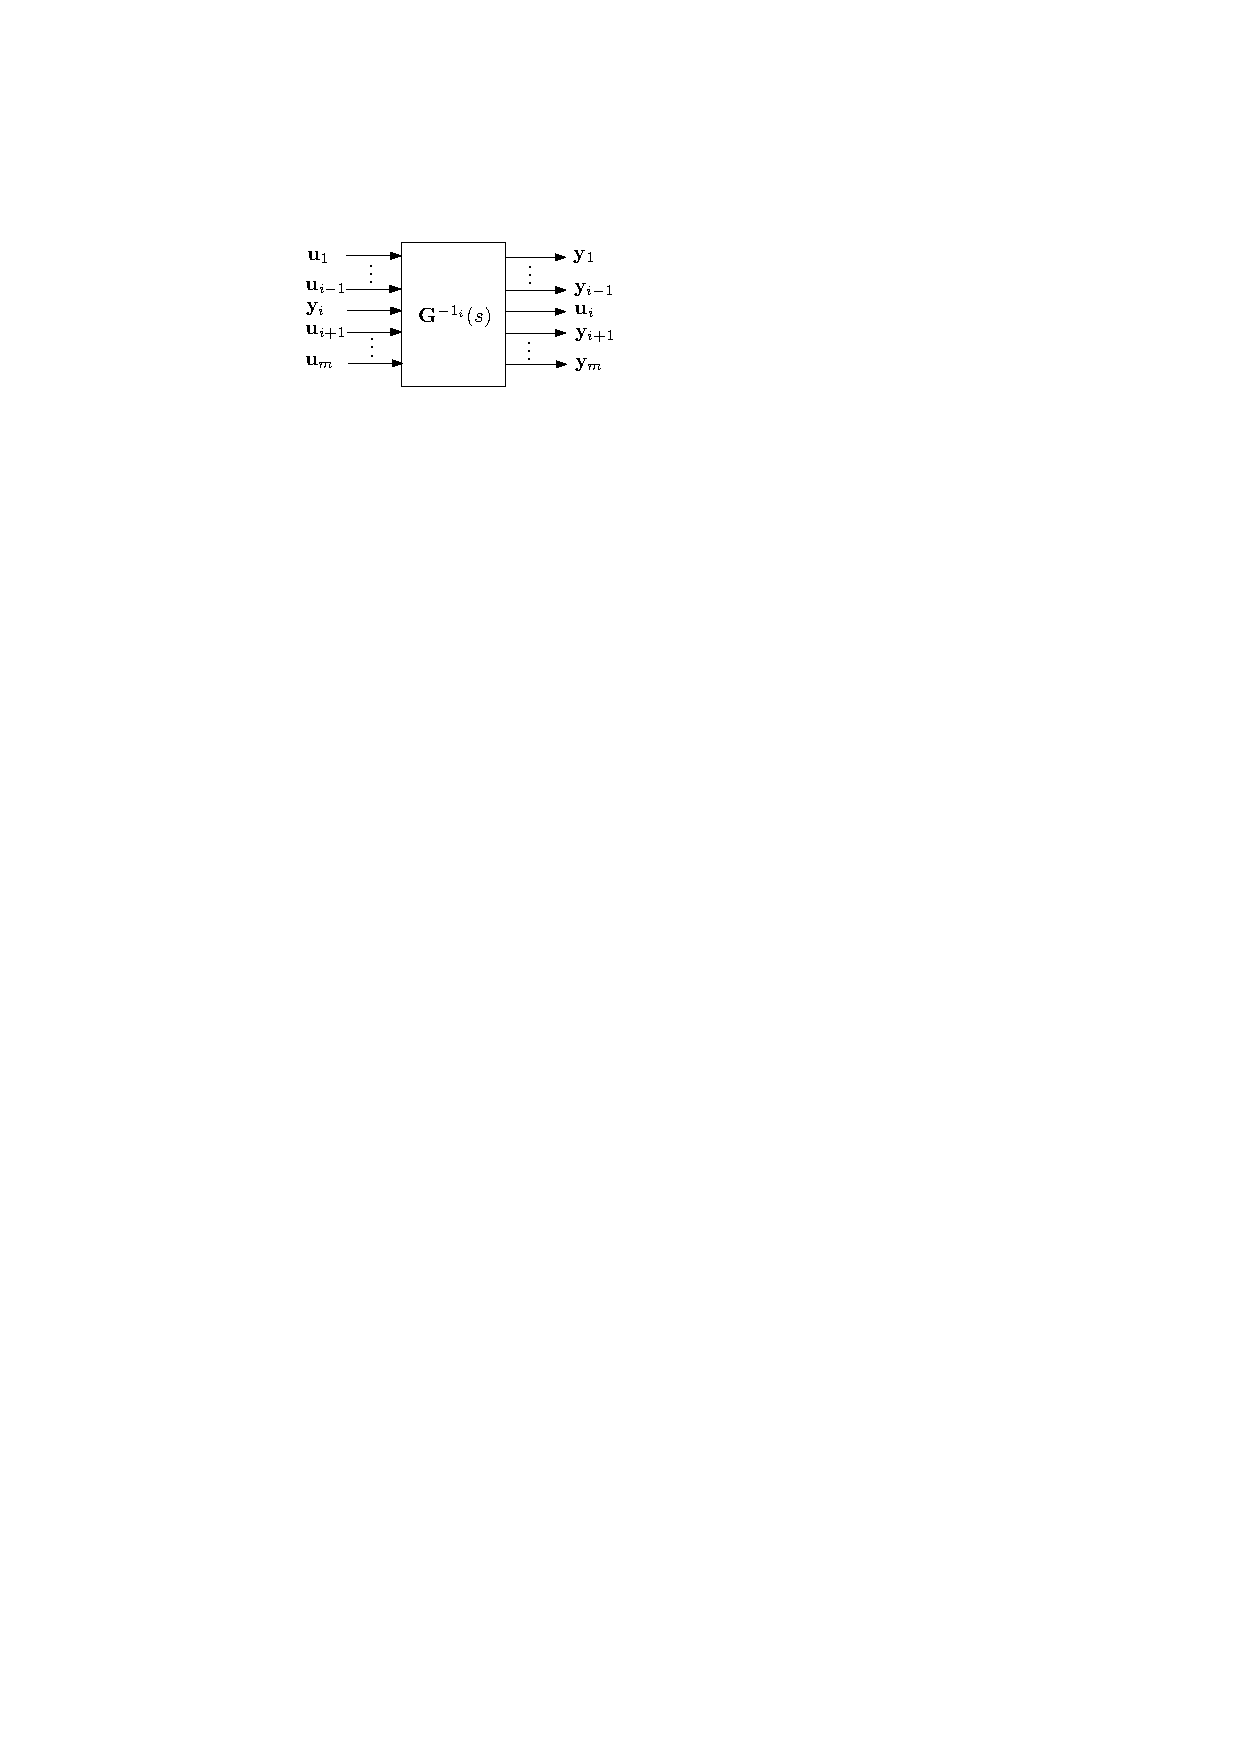
\includegraphics[width=0.4\textwidth]{inv1c}
\caption{Inversion of the $i$-th channel of $\mathbf{G}$.}
\label{fig:inv1c} 
\end{figure}


\paragraph{Multi channel inversion:} Let $\mathbf{I}$ be the vector (with $q$ components) of indices corresponding to the channels to be inverted. The successive inversion of the $q$ channels in $\mathbf{G}(s)$ is denoted:
\begin{equation}
\mathbf{G}^{-1_{\mathbf{I}}}(s)=\left[\left[\left[\mathbf{G}^{-1_{\mathbf{I}(1)}}\right]^{-1_{\mathbf{I}(2)}}\right]^{\cdots}\right]^{-1_{\mathbf{I}(q)}}(s)\;.
\end{equation}

\section*{Appendix 2: TITOP model of the \textsc{Euler-Bernoulli} beam under various boundary conditions}
%\FloatBarrier
\paragraph{Case \# 1: free-free beam (Fig. \ref{fig:Tff}).} The model $\mathbf{G}_{f,pol}^{-1_{[3,4]}}(s)$ is  used to set to $0$ its inputs: $F^y_c$, $T^z_c$, $F^y_P$, and $T^z_P$. The augmented model with the $2$ rigid modes is depicted in Fig. \ref{fig:Tff} (right).
\begin{figure}[htbp!]
  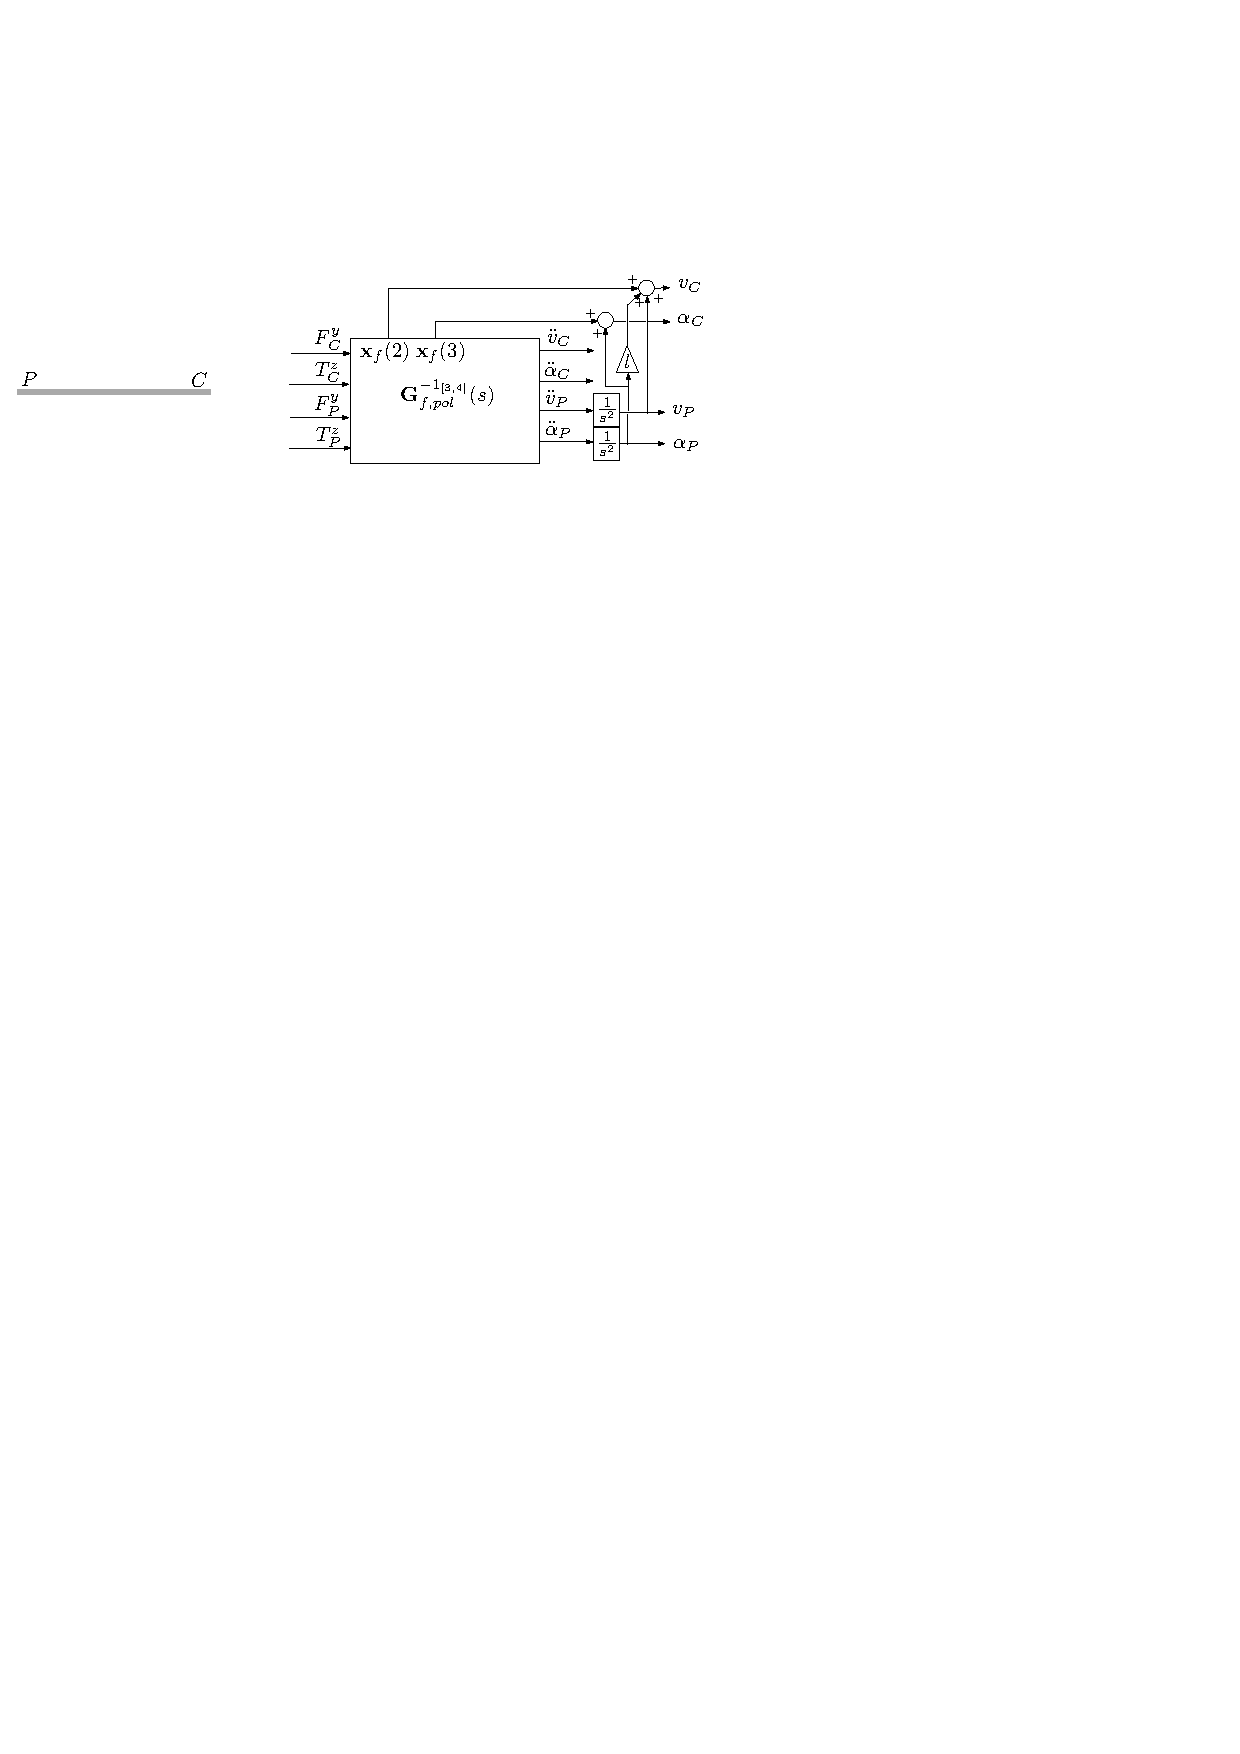
\includegraphics[width=0.8\textwidth]{Tffb}
\caption{The free-free beam (left) and its block-diagram model (right).}
\label{fig:Tff} 
\end{figure}
\begin{table}[htbp!]
% table caption is above the table
\caption{The first two natural frequencies $\omega_i$ of the free-free beam model $\mathbf{G}_{f,pol}^{-1_{[3,4]}}(s)$ and the relative errors with the reference values $\omega_{i,ref}$.}
\label{tab:Tff}       % Give a unique label
% For LaTeX tables use
\begin{tabular}{llll}
\hline\noalign{\smallskip}
  $i$ & $\omega_{i,ref}\,\left(\sqrt{\frac{EI_z}{\rho S l^4}}\right)$ &  $\omega_i\,\left(\sqrt{\frac{EI_z}{\rho S l^4}}\right)$ &  $\Delta \omega_i\,(\%)$ \\
\noalign{\smallskip}\hline\noalign{\smallskip}
$1$ & $22.373$ & $22.564$  & $0.85$ \\ 
$2$ & $61.673$ & $63.537$ & $3.0$ \\
\hline
\end{tabular}
\end{table}

\FloatBarrier
\paragraph{Case \# 2: clamped-clamped beam (Fig. \ref{fig:Tcc}).} The model $\mathbf{G}_{f,pol}^{-1_{[1,2]}}(s)$ is used to set to $0$ its inputs: $\ddot{v}_C$, $\ddot{\alpha}_C$, $\ddot{v}_P$, and $\ddot{\alpha}_P$. There is no rigid modes in this case. The internal state constraints:
\[
\widetilde{v}(l)=\vec{x}_f(2)=0,\;\widetilde{v}'(l)=\vec{x}_f(3)=0\;\forall\,t\;\Rightarrow\;\dot{\vec{x}}_f(2)=\dot{\vec{x}}_f(3)=\dot{\vec{x}}_f(6)=\dot{\vec{x}}_f(7)=0
\]
can be used to truncate the state-space representation of $\mathbf{G}_{f,pol}^{-1_{[1,2]}}(s)$ to a $4$-th order model. The frequencies of the 2 flexible modes are displayed in Table \ref{tab:Tcc}.
\begin{figure}[htbp!]
  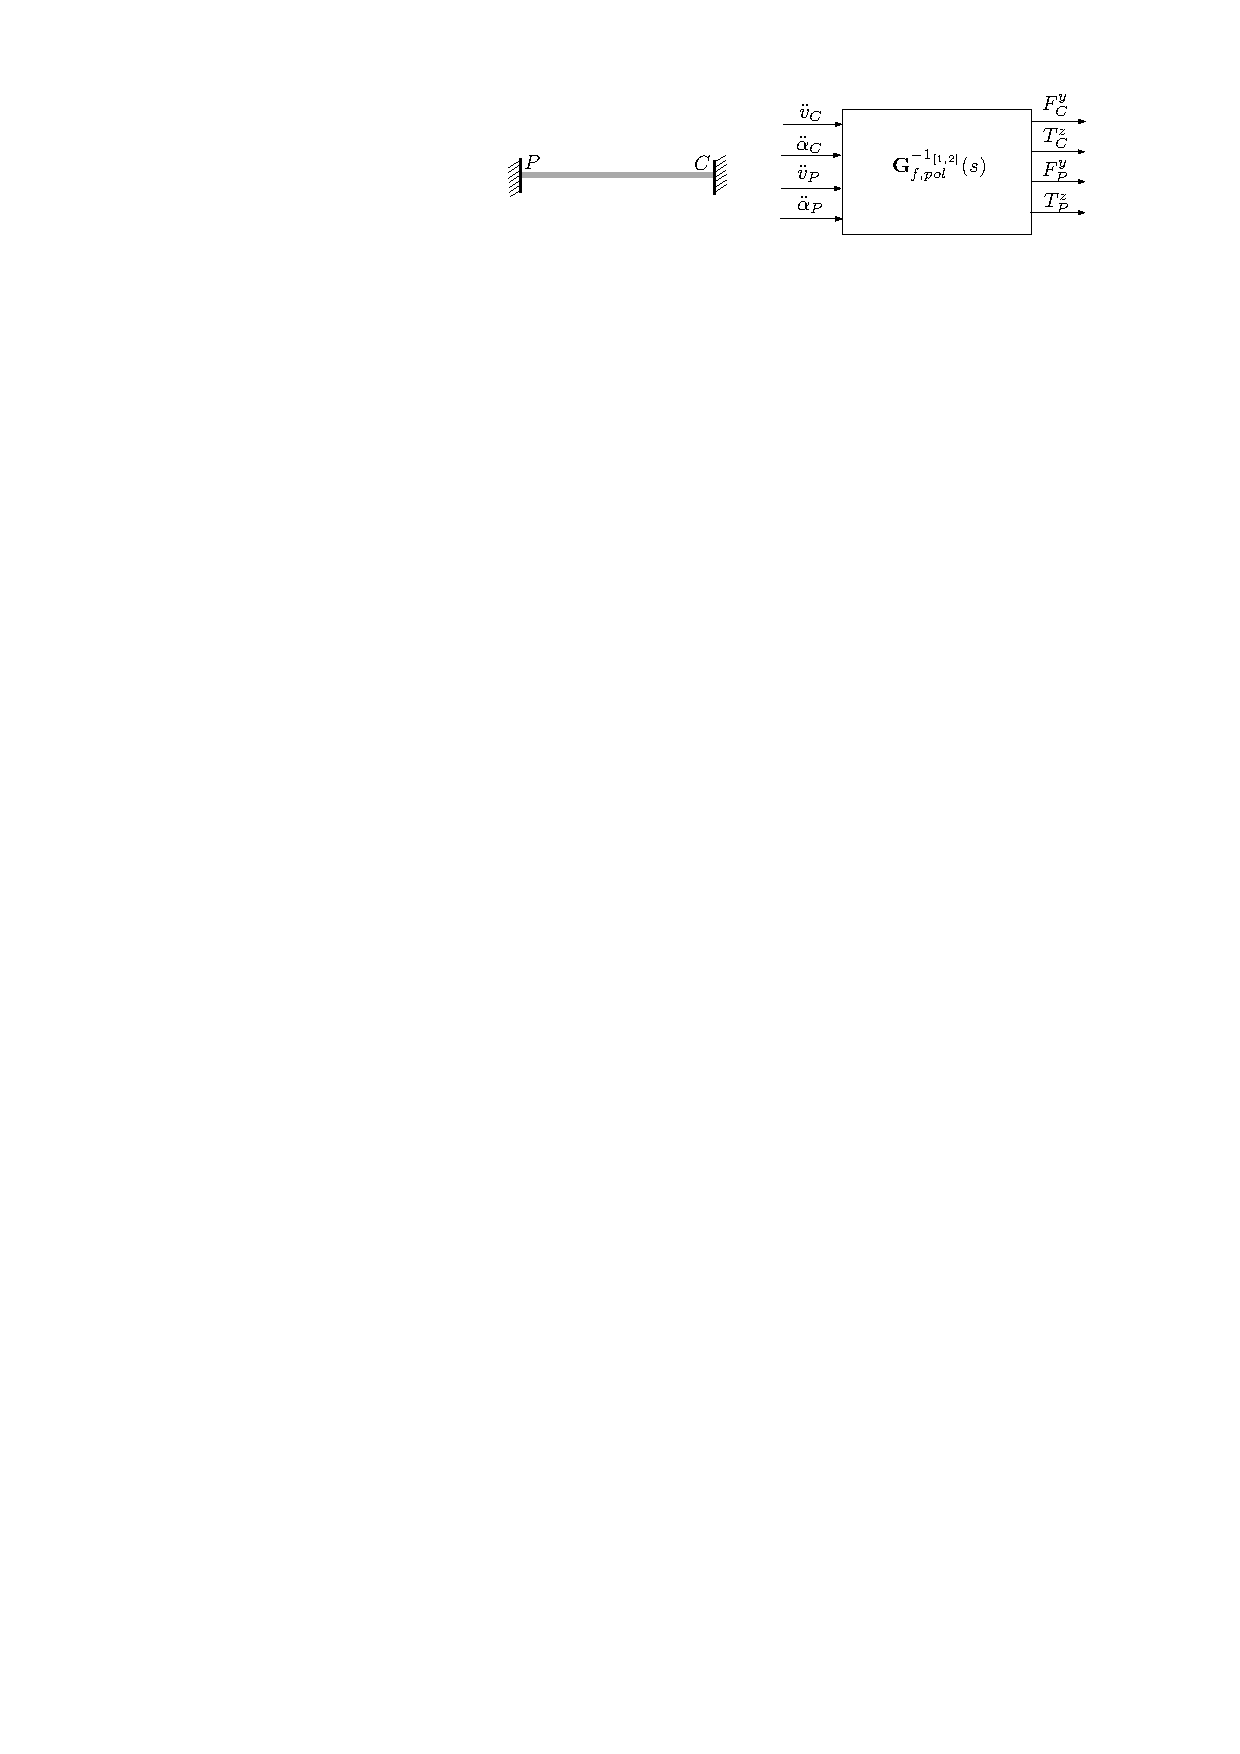
\includegraphics[width=0.7\textwidth]{Tccb}
\caption{The clamped-clamped beam (left) and its block-diagram model (right).}
\label{fig:Tcc} 
\end{figure}
\begin{table}[htbp!]
% table caption is above the table
\caption{The first two natural frequencies $\omega_i$ of the clamped-clamped beam model $\mathbf{G}_{f,pol}^{-1_{[1,2]}}(s)$ and the relative errors with the reference values $\omega_{i,ref}$.}
\label{tab:Tcc}       % Give a unique label
% For LaTeX tables use
\begin{tabular}{llll}
\hline\noalign{\smallskip}
  $i$ & $\omega_{i,ref}\,\left(\sqrt{\frac{EI_z}{\rho S l^4}}\right)$ &  $\omega_i\,\left(\sqrt{\frac{EI_z}{\rho S l^4}}\right)$ &  $\Delta \omega_i\,(\%)$ \\
\noalign{\smallskip}\hline\noalign{\smallskip}
$1$ & $22.373$ & $22.45$  & $0.34$ \\ 
$2$ & $61.673$ & $62.929$ & $2.0$ \\
\hline
\end{tabular}
\end{table}

\FloatBarrier
\paragraph{Case \# 3: pinned-free beam (Fig. \ref{fig:Tpf}).} The model $\mathbf{G}_{f,pol}^{-1_{4}}(s)$ is used to set to $0$ its inputs: $F^y_C$, $T^z_C$, $\ddot{v}_P$, and $T^z_P$. The augmented model with the rigid mode is depicted in Fig. \ref{fig:Tpf} (right).
\begin{figure}[htbp!]
  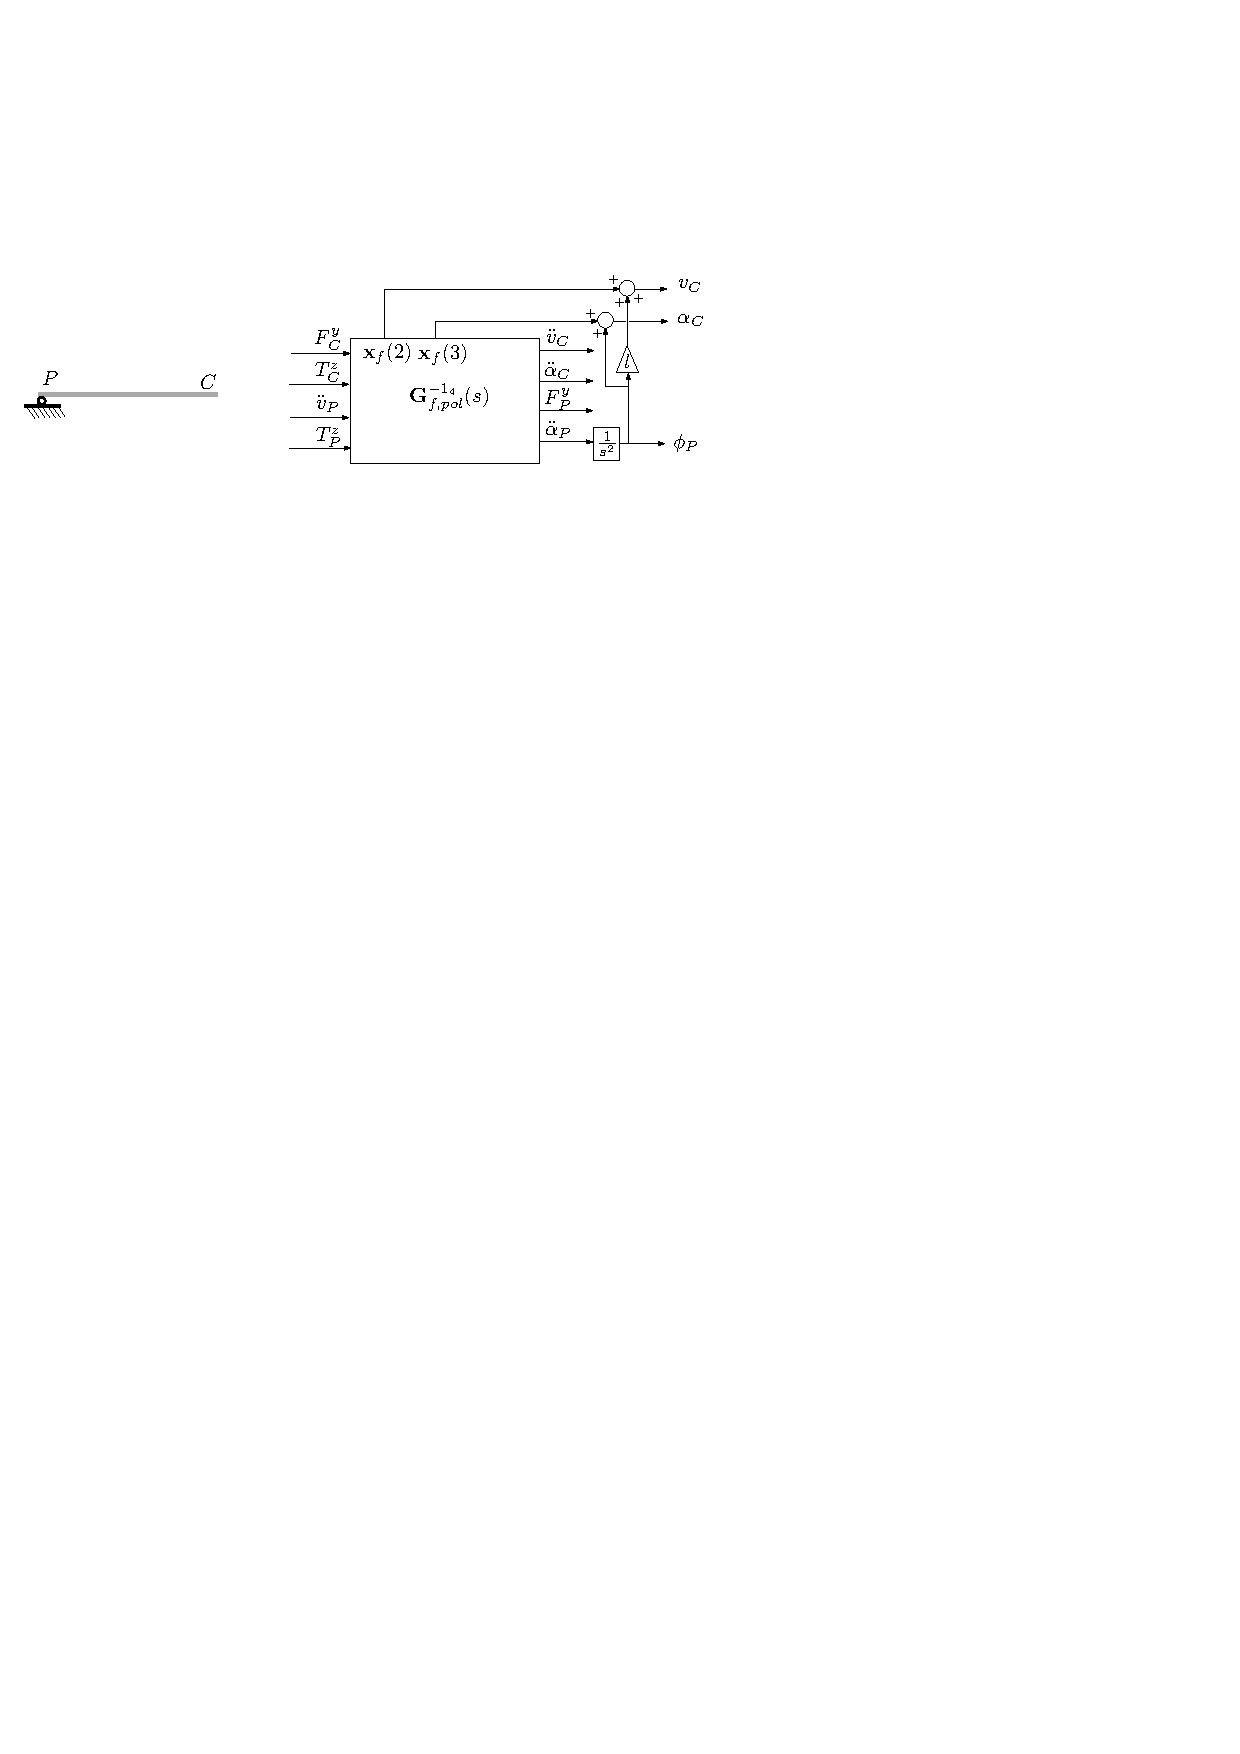
\includegraphics[width=0.8\textwidth]{Tpfb}
\caption{The pinned-free beam (left) and its block-diagram model (right).}
\label{fig:Tpf} 
\end{figure}
\begin{table}[htbp!]
% table caption is above the table
\caption{The first two natural frequencies $\omega_i$ of the pinned-free beam model $\mathbf{G}_{f,pol}^{-1_{4}}(s)$ and the relative errors with the reference values $\omega_{i,ref}$.}
\label{tab:Tpf}       % Give a unique label
% For LaTeX tables use
\begin{tabular}{llll}
\hline\noalign{\smallskip}
  $i$ & $\omega_{i,ref}\,\left(\sqrt{\frac{EI_z}{\rho S l^4}}\right)$ &  $\omega_i\,\left(\sqrt{\frac{EI_z}{\rho S l^4}}\right)$ &  $\Delta \omega_i\,(\%)$ \\
\noalign{\smallskip}\hline\noalign{\smallskip}
$1$ & $15.418$ & $15.445$  & $0.17$ \\ 
$2$ & $49.965$ & $51:206$ & $2.5$ \\
\hline
\end{tabular}
\end{table}


\FloatBarrier
\paragraph{Case \# 4: pinned-clamped beam (see Fig. \ref{fig:Tpc}).} The model $\mathbf{G}_{f,pol}^{-1_{[1,2,4]}}(s)$ is used to set to $0$ its inputs: $\ddot{v}_C$, $\ddot{\alpha}_C$, $\ddot{v}_P$, and $T^z_P$. There is no rigid modes in this case. The internal state constraints:
\[
\widetilde{v}(l)-l\widetilde{v}'(l)=\vec{x}_f(2)-l\vec{x}_f(3)=0\;\forall\,t\;\Rightarrow\;\dot{\vec{x}}_f(2)-l\dot{\vec{x}}_f(3)=\dot{\vec{x}}_f(6)-l\dot{\vec{x}}_f(7)=0
\]
can be used to reduce the state-space representation of $\mathbf{G}_{f,pol}^{-1_{[1,2,4]}}(s)$ to a $6$-th order model.
\begin{figure}[htbp!]
  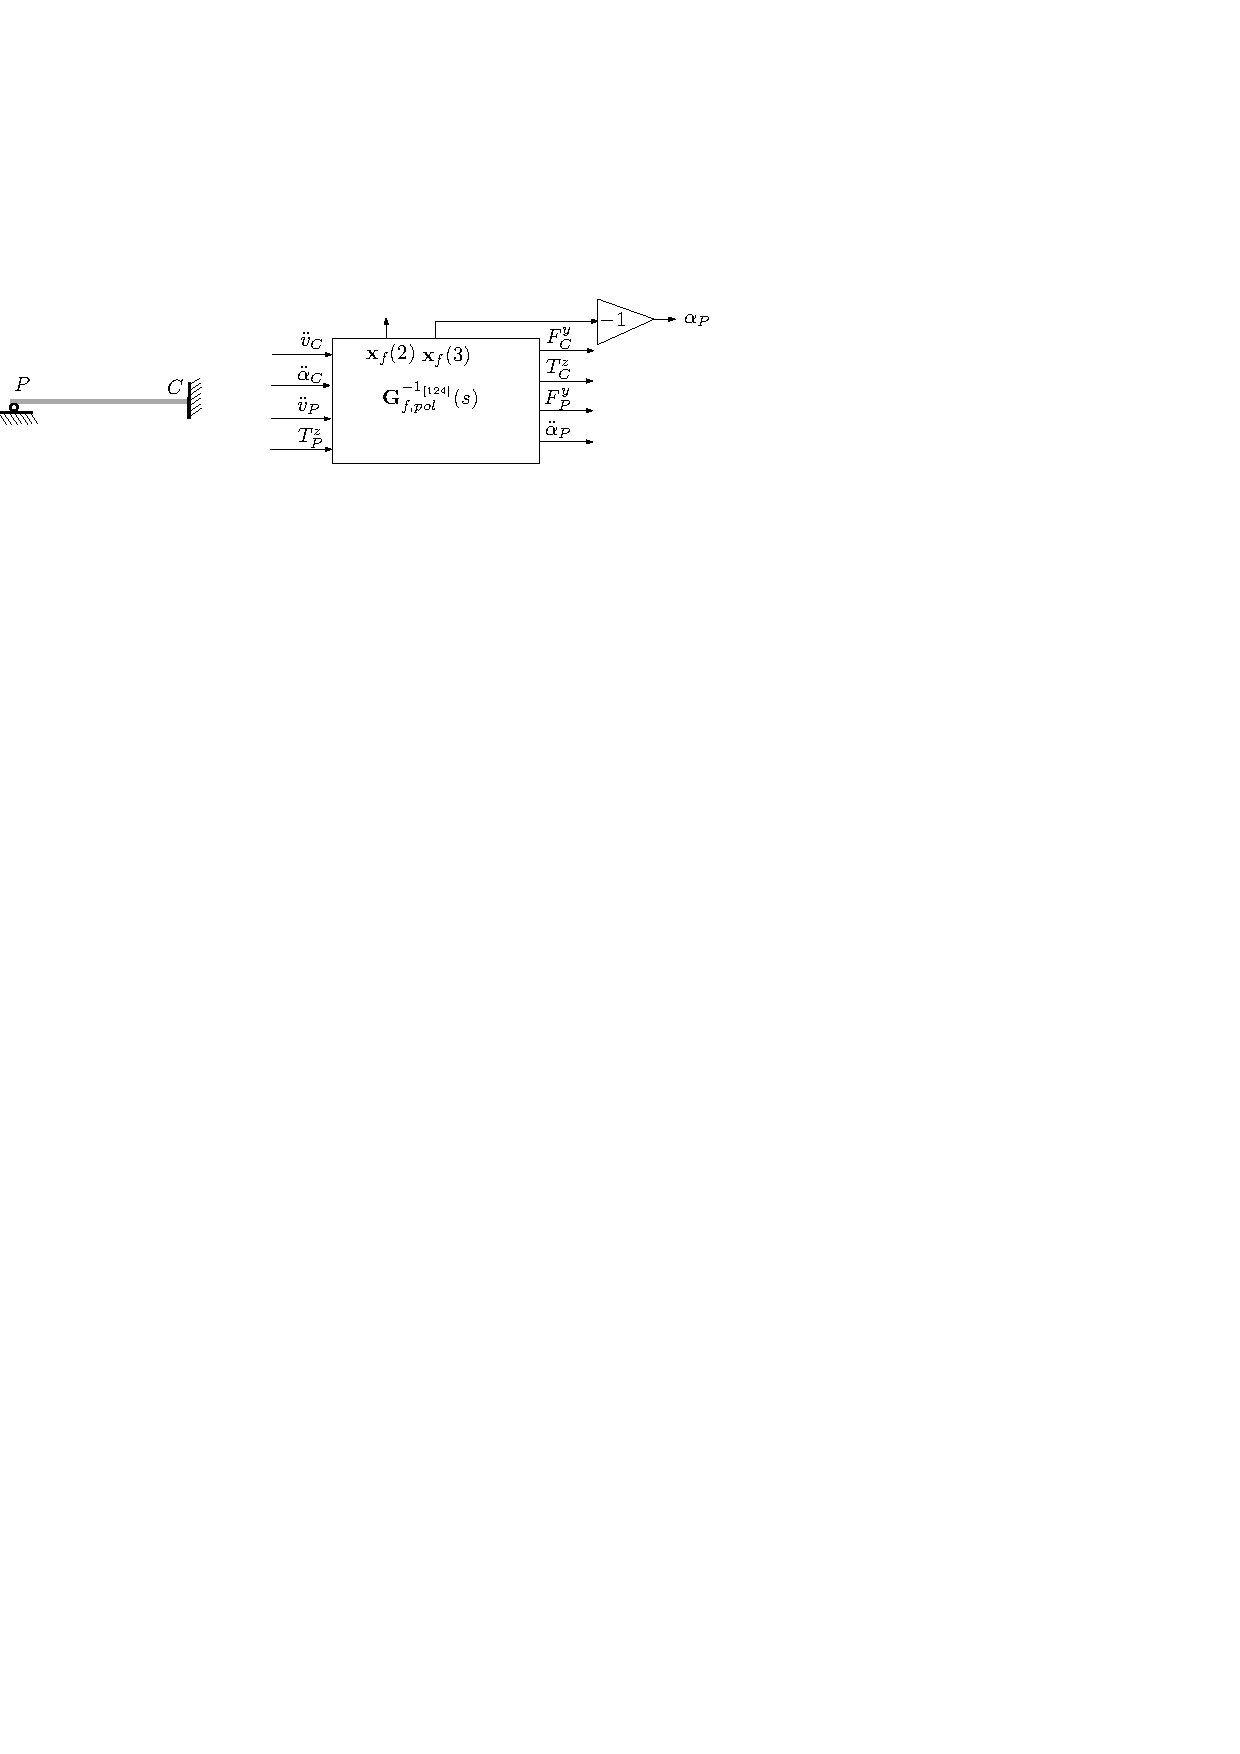
\includegraphics[width=0.8\textwidth]{Tpcb}
\caption{The pinned-clamped beam (right) and its block-diagram model (left).}
\label{fig:Tpc} 
\end{figure}
\begin{table}[htbp!]
% table caption is above the table
\caption{The first two natural frequencies $\omega_i$ of the pinned-clamped beam model $\mathbf{G}_{f,pol}^{-1_{[1,2,4]}}(s)$ and the relative errors with the reference values $\omega_{i,ref}$.}
\label{tab:Tpc}       % Give a unique label
% For LaTeX tables use
\begin{tabular}{llll}
\hline\noalign{\smallskip}
  $i$ & $\omega_{i,ref}\,\left(\sqrt{\frac{EI_z}{\rho S l^4}}\right)$ &  $\omega_i\,\left(\sqrt{\frac{EI_z}{\rho S l^4}}\right)$ &  $\Delta \omega_i\,(\%)$ \\
\noalign{\smallskip}\hline\noalign{\smallskip}
$1$ & $15.418$ & $15.433$  & $0.1$ \\ 
$2$ & $49.965$ & $50.724$ & $1.5$ \\
\hline
\end{tabular}
\end{table}

\FloatBarrier
\paragraph{Case \# 5: pinned-pinned beam (Fig. \ref{fig:Tpp}).} The model $\mathbf{G}_{f,pol}^{-1_{[1,4]}}(s)$ is used to set to $0$ its inputs: $\ddot{v}_C$, $T^z_c$, $\ddot{v}_P$, and $T^z_P$. There is no rigid modes in this case.
\begin{figure}[htbp!]
  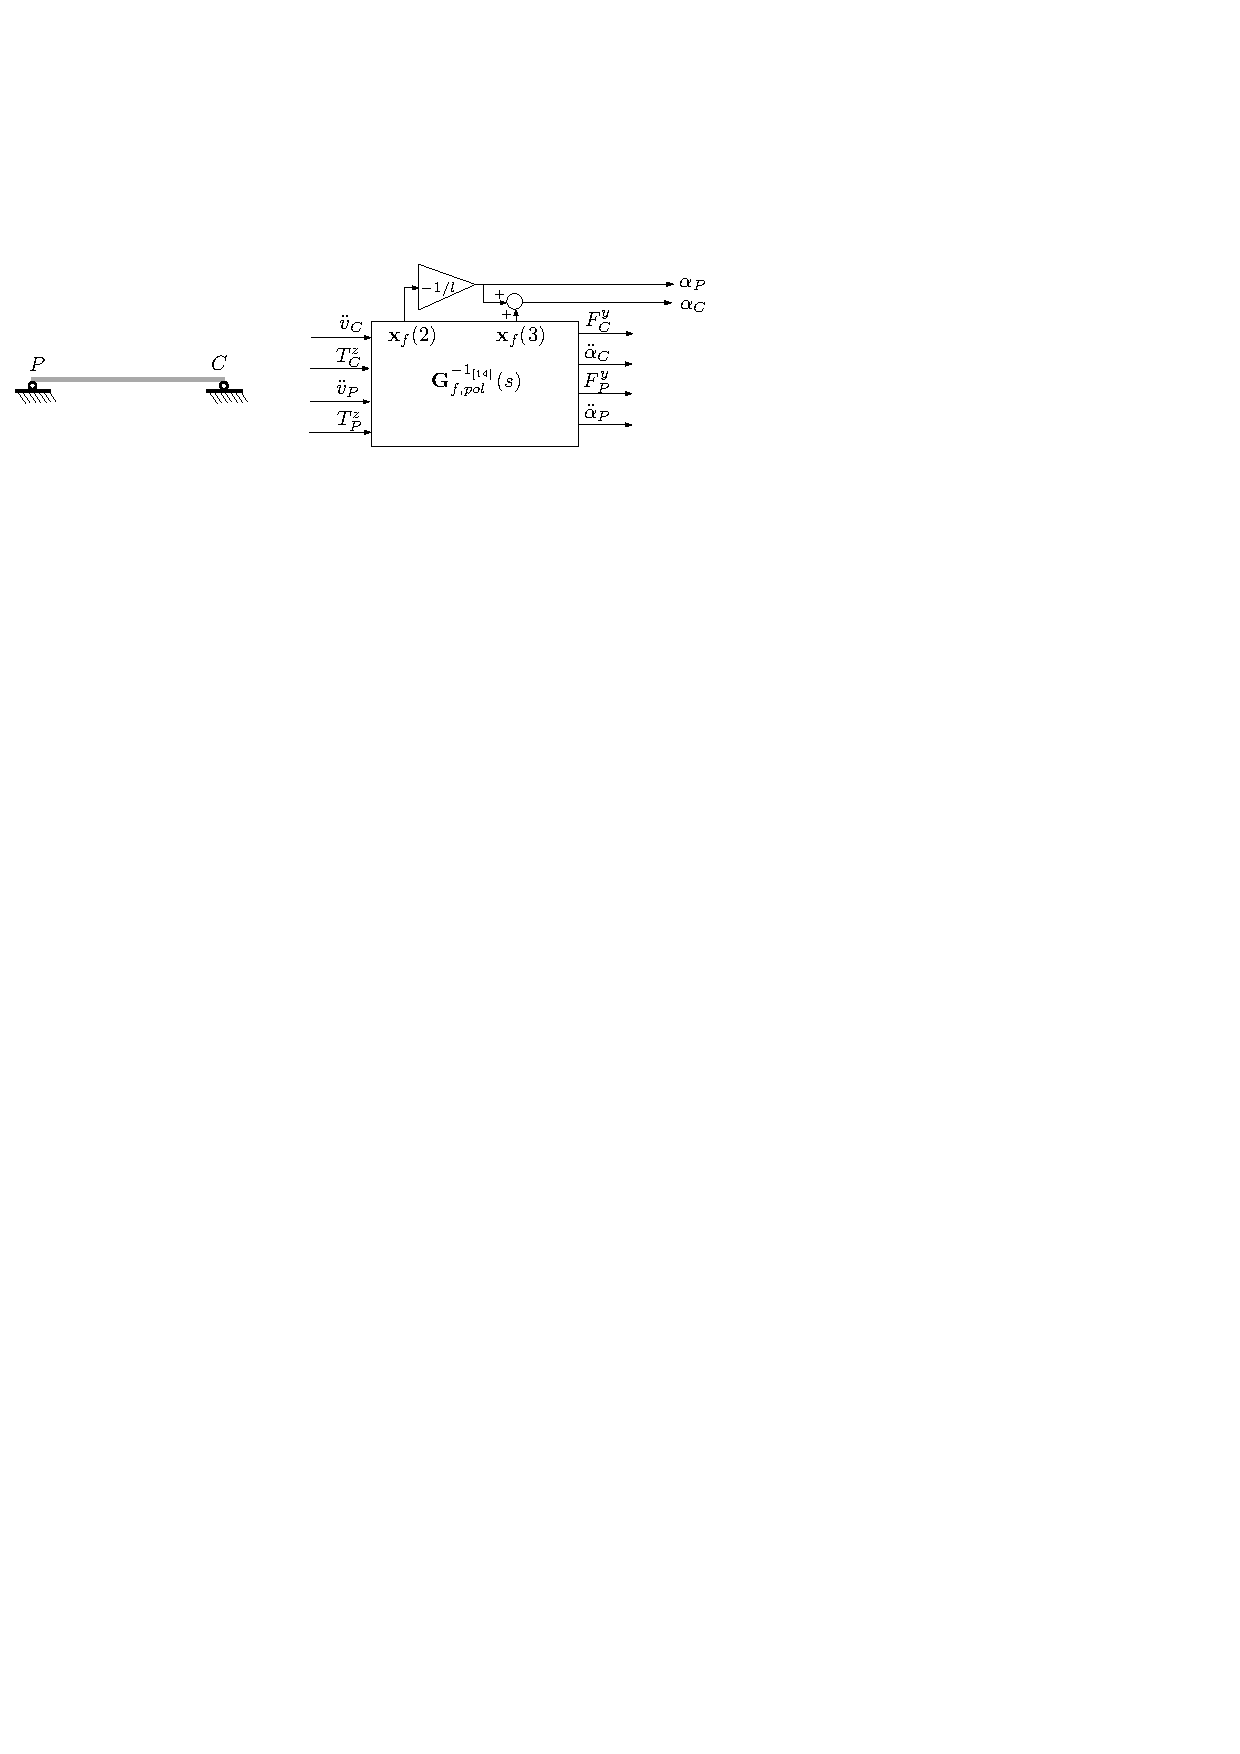
\includegraphics[width=0.8\textwidth]{Tppb}
\caption{The pinned-pinned beam (left) and its block-diagram model (right).}
\label{fig:Tpp} 
\end{figure}
\begin{table}[htbp!]
% table caption is above the table
\caption{The first two natural frequencies $\omega_i$ of the pinned-pinned beam model $\mathbf{G}_{f,pol}^{-1_{[1,4]}}(s)$ and the relative errors with the reference values $\omega_{i,ref}$.}
\label{tab:Tpp}       % Give a unique label
% For LaTeX tables use
\begin{tabular}{llll}
\hline\noalign{\smallskip}
  $i$ & $\omega_{i,ref}\,\left(\sqrt{\frac{EI_z}{\rho S l^4}}\right)$ &  $\omega_i\,\left(\sqrt{\frac{EI_z}{\rho S l^4}}\right)$ &  $\Delta \omega_i\,(\%)$ \\
\noalign{\smallskip}\hline\noalign{\smallskip}
$1$ & $9.8696$ & $9.8725$  & $0.03$ \\ 
$2$ & $39.478$ & $39.646$ & $0.4$ \\
\hline
\end{tabular}
\end{table}

\FloatBarrier
\paragraph{Case \# 6: sliding-free beam (Fig. \ref{fig:Tsf}).} The model $\mathbf{G}_{f,pol}^{-1_{3}}(s)$ is used to set to $0$ its inputs: $F^y_c$, $T^z_c$, $F^y_P$, and $\ddot{\alpha}_P$. The augmented model with the rigid mode is depicted in Fig. \ref{fig:Tsf} (right).
\begin{figure}[htbp!]
  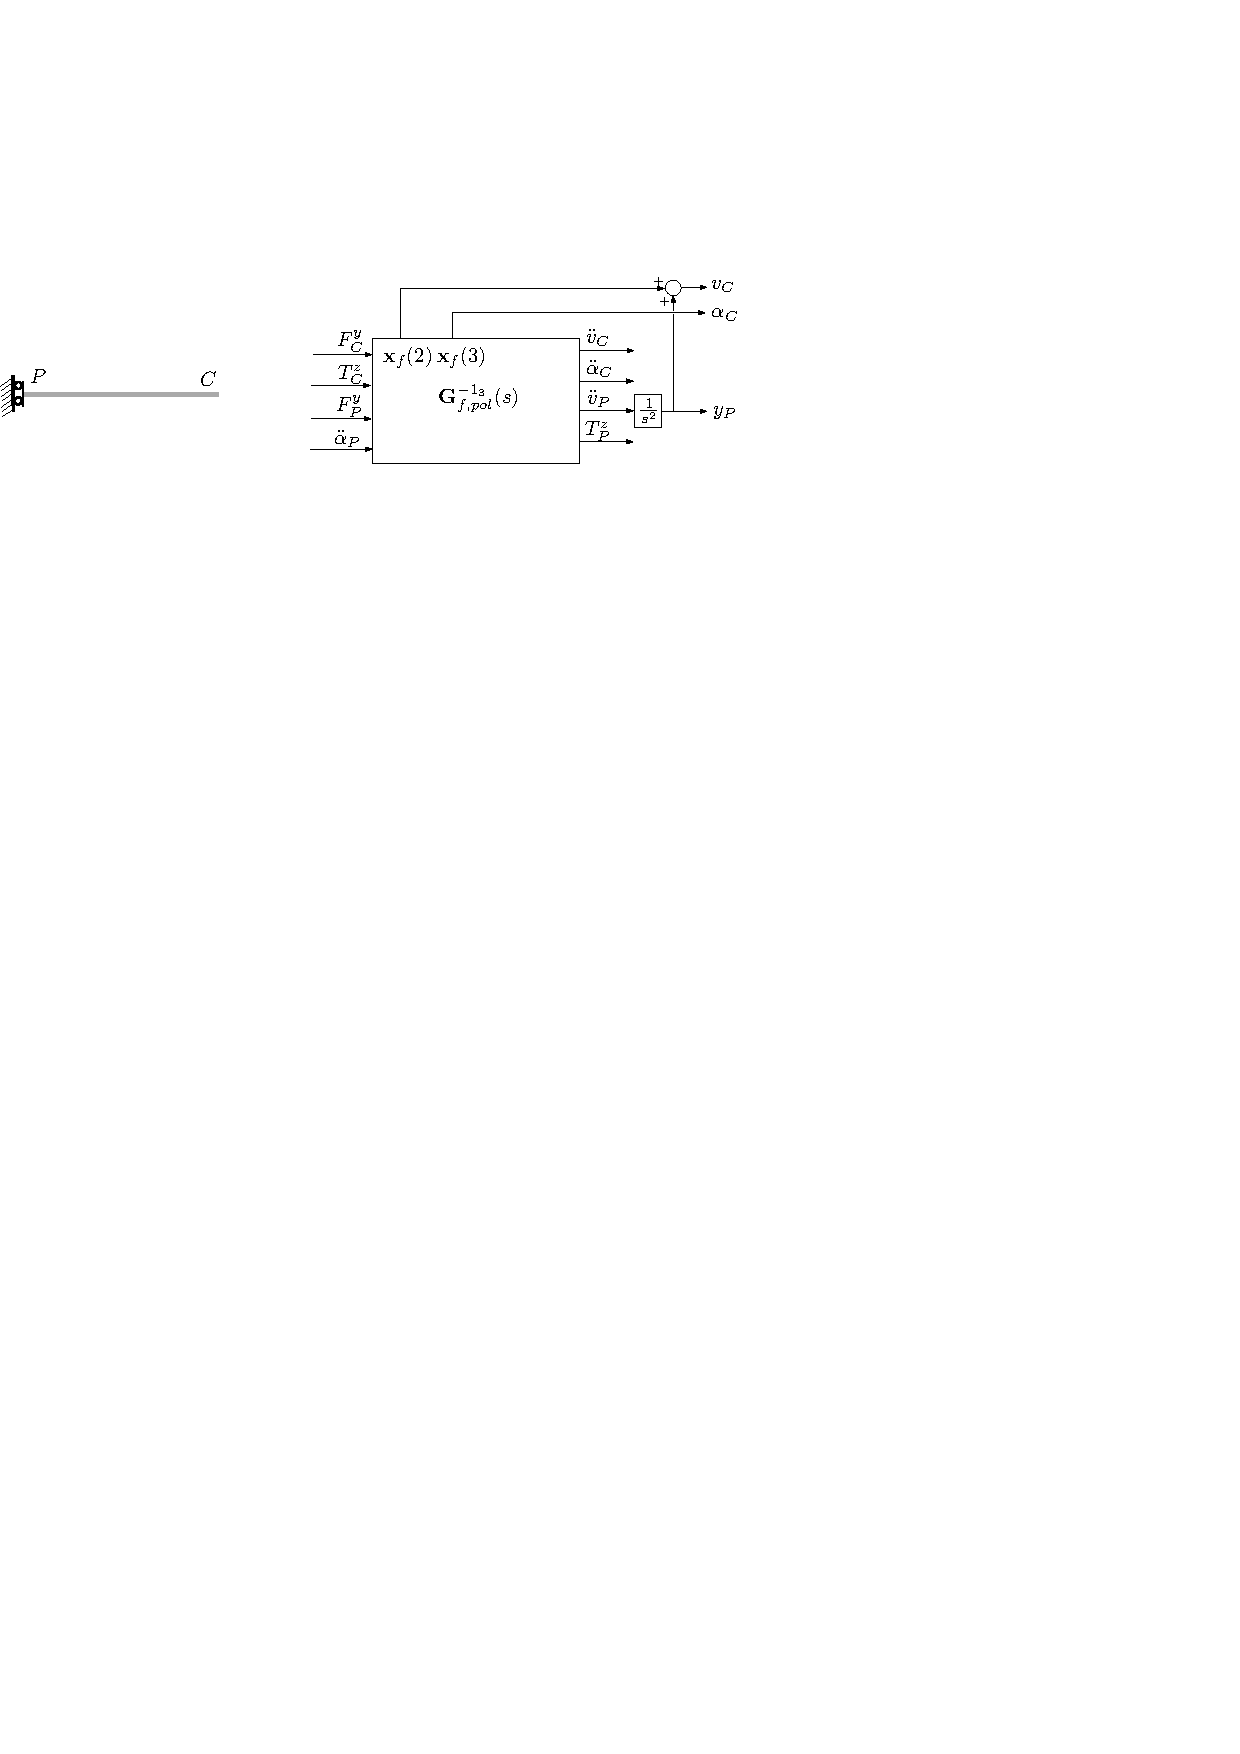
\includegraphics[width=0.8\textwidth]{Tsfb}
\caption{The sliding-free beam (left) and its block-diagram model (right).}
\label{fig:Tsf} 
\end{figure}
\begin{table}[htbp!]
% table caption is above the table
\caption{The first two natural frequencies $\omega_i$ of the sliding-free beam model $\mathbf{G}_{f,pol}^{-1_{3}}(s)$ and the relative errors with the reference values $\omega_{i,ref}$.}
\label{tab:Tsf}       % Give a unique label
% For LaTeX tables use
\begin{tabular}{llll}
\hline\noalign{\smallskip}
  $i$ & $\omega_{i,ref}\,\left(\sqrt{\frac{EI_z}{\rho S l^4}}\right)$ &  $\omega_i\,\left(\sqrt{\frac{EI_z}{\rho S l^4}}\right)$ &  $\Delta \omega_i\,(\%)$ \\
\noalign{\smallskip}\hline\noalign{\smallskip}
$1$ & $5.5932$ & $5.5934$  & $0.003$ \\ 
$2$ & $30.226$ & $30.734$ & $1.7$ \\
\hline
\end{tabular}
\end{table}

\FloatBarrier
\paragraph{Case \# 7: sliding-clamped beam (see Fig. \ref{fig:Tsc}).} The model $\mathbf{G}_{f,pol}^{-1_{[1,2,3]}}(s)$ is used to set to $0$ its inputs: $\ddot{v}_C$, $\ddot{\alpha}_C$, $F^y_P$, and $\ddot{\alpha}_P$. There is no rigid modes in this case. The internal state constraints:
\[
\widetilde{v}'(l)=\vec{x}_f(3)=0\;\forall\,t\;\Rightarrow\;\dot{\vec{x}}_f(3)=\dot{\vec{x}}_f(7)=0
\]
can be used to reduce the state-space representation of $\mathbf{G}_{f,pol}^{-1_{[1,2,3]}}(s)$ to a $6$-th order model.
\begin{figure}[htbp!]
  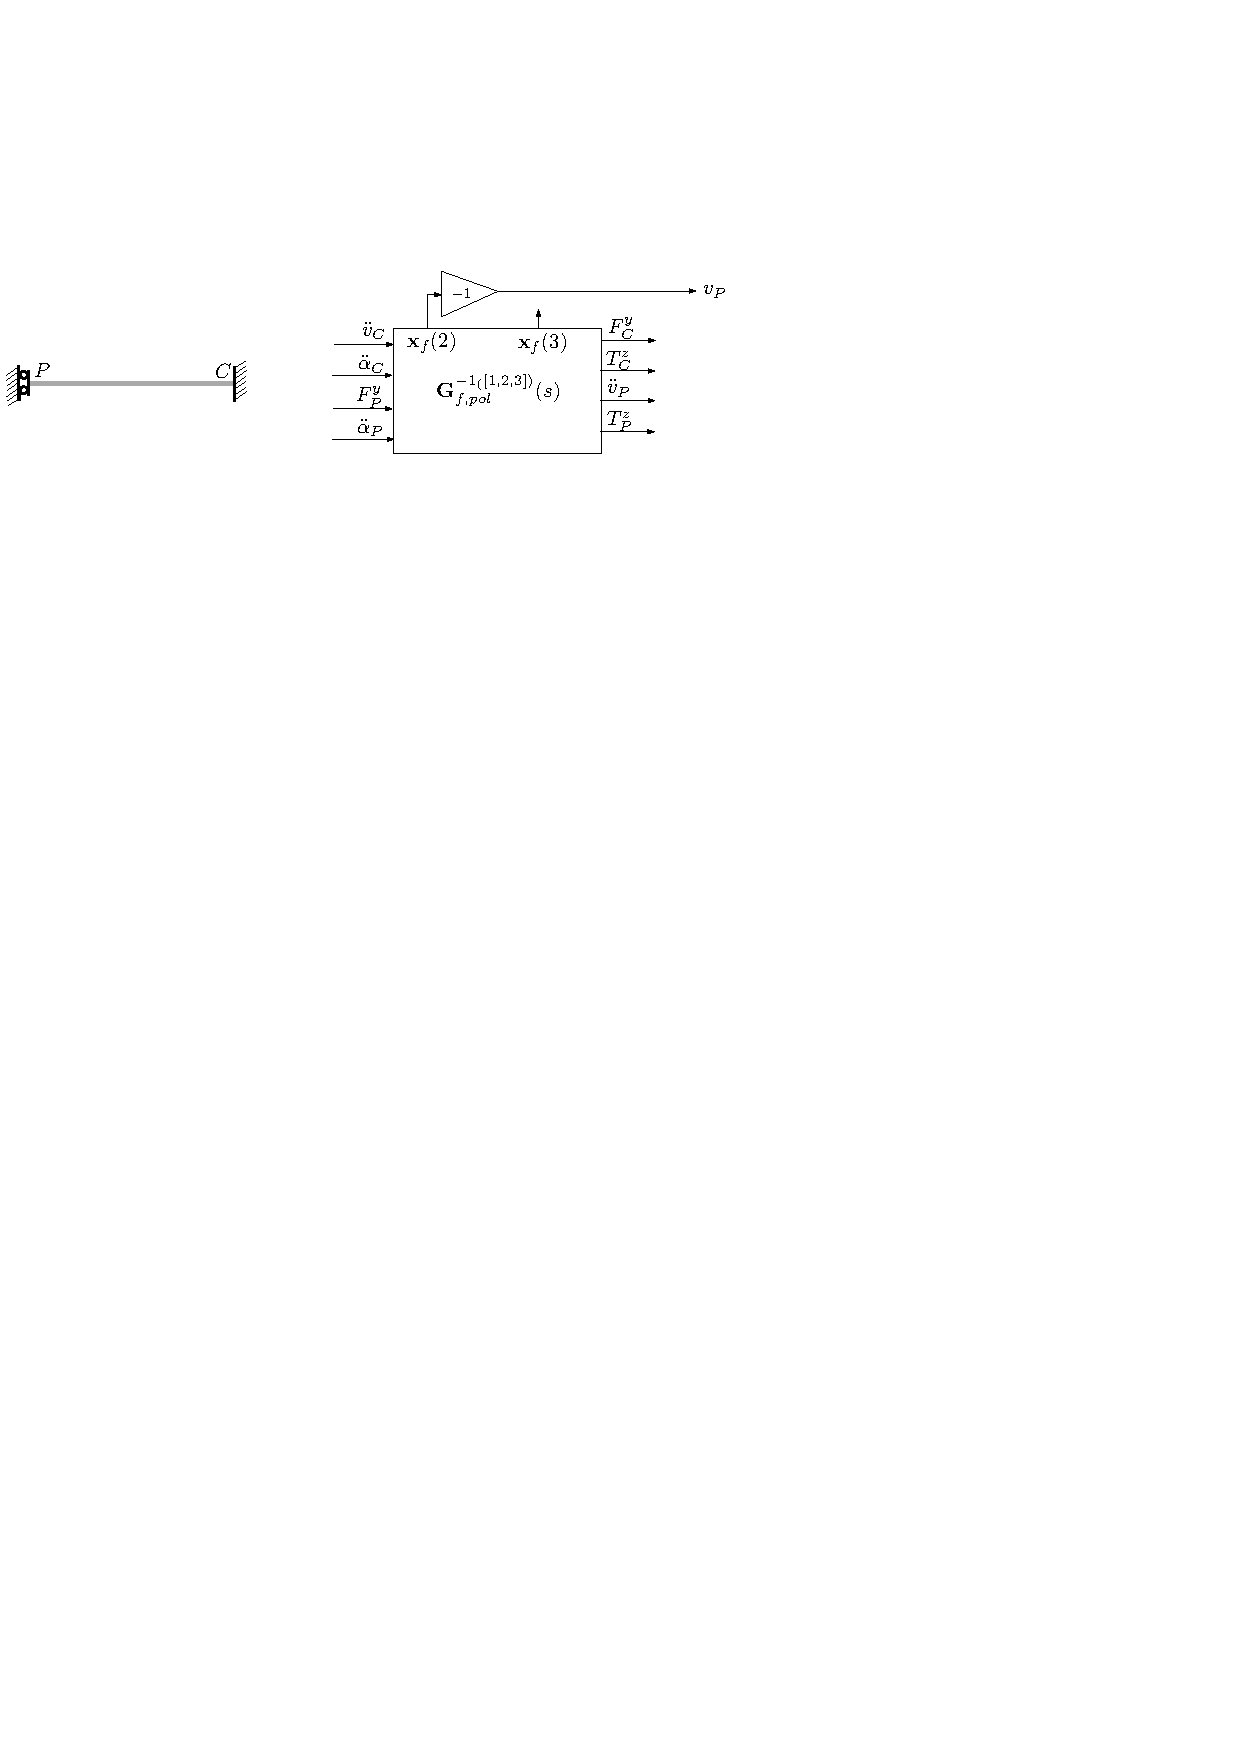
\includegraphics[width=0.8\textwidth]{Tscb}
\caption{The sliding-clamped beam (right) and its block-diagram model (left).}
\label{fig:Tsc} 
\end{figure}
\begin{table}[htbp!]
% table caption is above the table
\caption{The first two natural frequencies $\omega_i$ of the sliding-clamped beam model $\mathbf{G}_{f,pol}^{-1_{[1,2,3]}}(s)$ and the relative errors with the reference values $\omega_{i,ref}$.}
\label{tab:Tsc}       % Give a unique label
% For LaTeX tables use
\begin{tabular}{llll}
\hline\noalign{\smallskip}
  $i$ & $\omega_{i,ref}\,\left(\sqrt{\frac{EI_z}{\rho S l^4}}\right)$ &  $\omega_i\,\left(\sqrt{\frac{EI_z}{\rho S l^4}}\right)$ &  $\Delta \omega_i\,(\%)$ \\
\noalign{\smallskip}\hline\noalign{\smallskip}
$1$ & $5.5932$ & $5.5933$  & $0.002$ \\ 
$2$ & $30.226$ & $30.561$ & $1.1$ \\
\hline
\end{tabular}
\end{table}

\FloatBarrier
\paragraph{Case \# 8:  sliding-pinned beam (see Fig. \ref{fig:Tsp}).} The model $\mathbf{G}_{f,pol}^{-1_{[1,3]}}(s)$ is used to set to $0$ its inputs: $\ddot{v}_C$, $T^z_C$, $F^y_P$, and $\ddot{\alpha}_P$. There is no rigid modes in this case.
\begin{figure}[htbp!]
  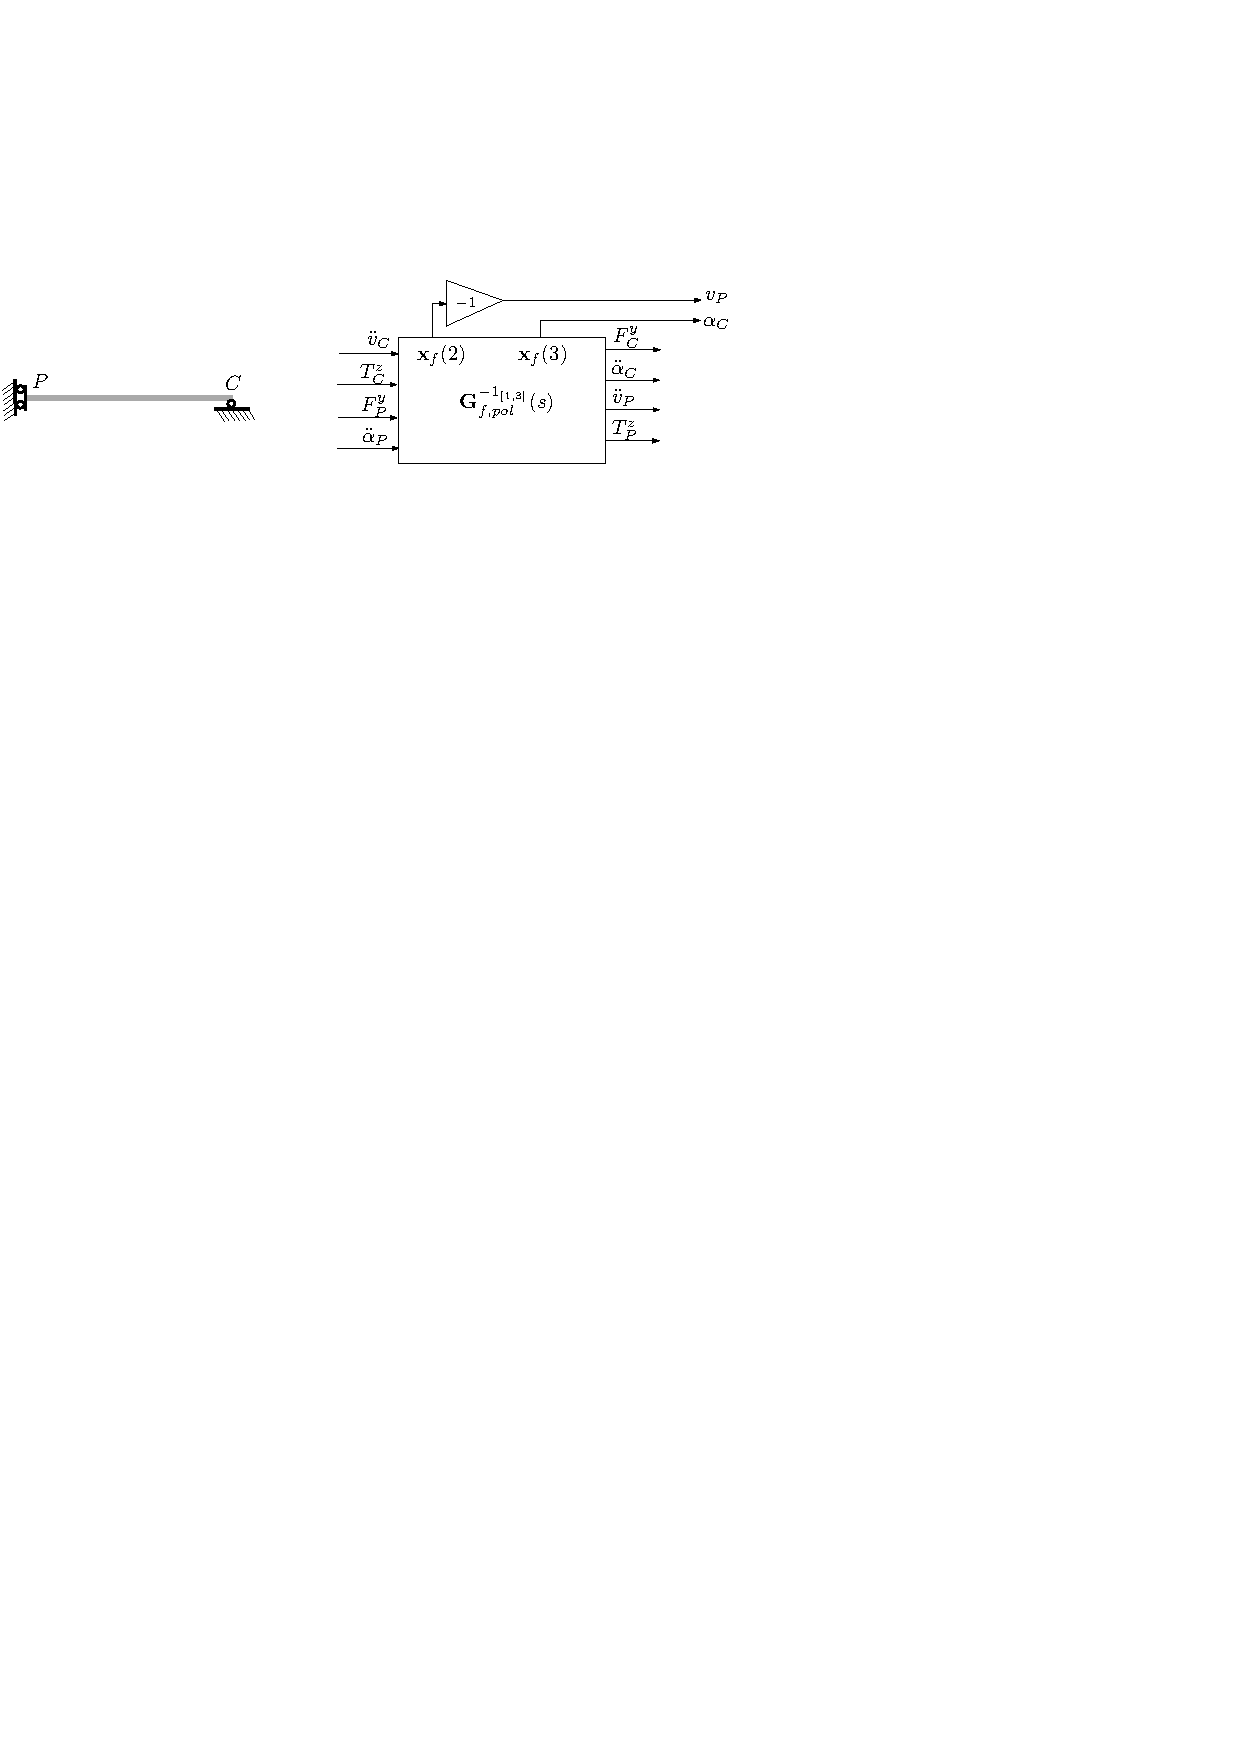
\includegraphics[width=0.8\textwidth]{Tspb}
\caption{The sliding-pinned beam (right) and its block-diagram model (left).}
\label{fig:Tsp} 
\end{figure}
\begin{table}[htbp!]
% table caption is above the table
\caption{The first two natural frequencies $\omega_i$ of the sliding-pinned beam model $\mathbf{G}_{f,pol}^{-1_{[1,3]}}(s)$ and the relative errors with the reference values $\omega_{i,ref}$.}
\label{tab:Tsp}       % Give a unique label
% For LaTeX tables use
\begin{tabular}{llll}
\hline\noalign{\smallskip}
  $i$ & $\omega_{i,ref}\,\left(\sqrt{\frac{EI_z}{\rho S l^4}}\right)$ &  $\omega_i\,\left(\sqrt{\frac{EI_z}{\rho S l^4}}\right)$ &  $\Delta \omega_i\,(\%)$ \\
\noalign{\smallskip}\hline\noalign{\smallskip}
$1$ & $2.4674$ & $2.4674$  & $0.0$ \\ 
$2$ & $22.207$ & $22.272$ & $0.3$ \\
\hline
\end{tabular}
\end{table}

\FloatBarrier
\paragraph{Case \# 9: sliding-sliding beam (Fig. \ref{fig:Tss}).} The model $\mathbf{G}_{f,pol}^{-1_{[2,3]}}(s)$ is used to set to $0$ its inputs: $F^y_c$, $\ddot{\alpha}_c$, $F^y_P$, and $\ddot{\alpha}_P$. The augmented model with the rigid mode is depicted in Fig. \ref{fig:Tss} (right).
\begin{figure}[htbp!]
  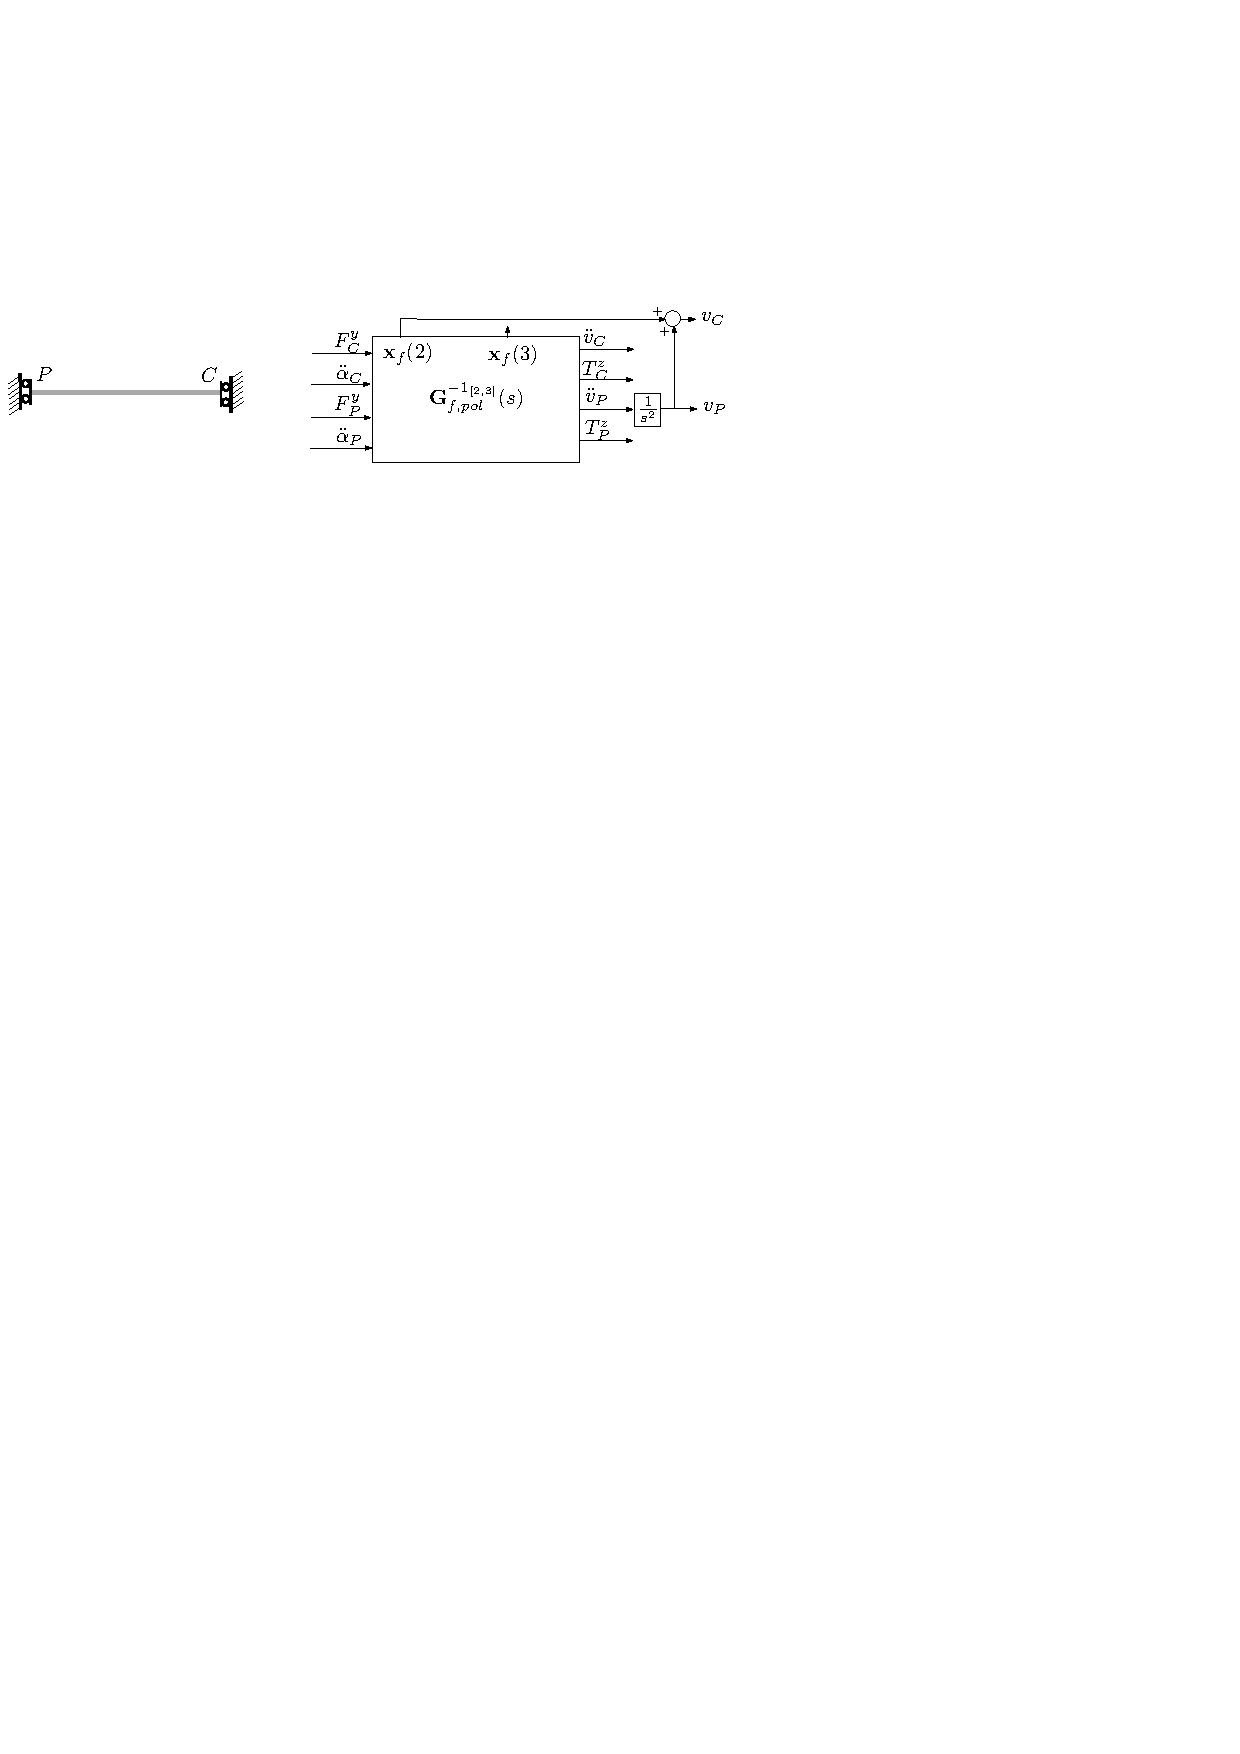
\includegraphics[width=0.8\textwidth]{Tssb}
\caption{The sliding-sliding beam (left) and its block-diagram model (right).}
\label{fig:Tss} 
\end{figure}
\begin{table}[htbp!]
% table caption is above the table
\caption{The first two natural frequencies $\omega_i$ of the sliding-sliding beam model $\mathbf{G}_{f,pol}^{-1_{[2,3]}}(s)$ and the relative errors with the reference values $\omega_{i,ref}$.}
\label{tab:Tss}       % Give a unique label
% For LaTeX tables use
\begin{tabular}{llll}
\hline\noalign{\smallskip}
  $i$ & $\omega_{i,ref}\,\left(\sqrt{\frac{EI_z}{\rho S l^4}}\right)$ &  $\omega_i\,\left(\sqrt{\frac{EI_z}{\rho S l^4}}\right)$ &  $\Delta \omega_i\,(\%)$ \\
\noalign{\smallskip}\hline\noalign{\smallskip}
$1$ & $9.8696$ & $9.8697$ & $0.0008$ \\ 
$2$ & $39.478$ & $40.988$ & $3.8$ \\
\hline
\end{tabular}
\end{table}

\FloatBarrier

\begin{acknowledgements}
This research is supported, in part, by ONERA (The French Aerospace Lab), CNES (The French Space Agency), ESA (European Space Agency), Thales Alenia Space and Polytechnique Montréal. We would like to thank more particularly \textsc{Christelle Cumer}, \textsc{Thomas Loquen}, \textsc{Christelle Pittet}, \textsc{Finn Ankersen}, \textsc{Luca Massotti}, \textsc{Catherine le Peuvédic}, \textsc{Chiara Toglia}, \textsc{David-Alexandre Saussié} and \textsc{Hari Murali}.
\end{acknowledgements}

% BibTeX users please use one of
%\bibliographystyle{spbasic}      % basic style, author-year citations
\bibliographystyle{spmpsci}      % mathematics and physical sciences
%\bibliographystyle{spphys}       % APS-like style for physics
\bibliography{biblio}   % name your BibTeX data base


\end{document}
% end of file template.tex

